\documentclass[12pt,a4paper,oneside]{report}
\usepackage{graphicx}
%\usepackage{german,a4}
\usepackage{lmodern}
\usepackage{fancyhdr}
\usepackage[utf8]{inputenc}
%\usepackage{setspace}
\usepackage[T1]{fontenc}
\usepackage{hyperref}
\usepackage[sf]{titlesec}
\usepackage{textcomp}
\usepackage{makeidx}
\usepackage{amsmath}
\usepackage[english, american]{babel}
\usepackage{listings}
\usepackage{color}
\usepackage{colortbl}
\definecolor{lightgray}{rgb}{0.8,0.8,0.8}
\definecolor{darkgreen}{rgb}{0,0.6,0}
\usepackage{pdfpages}
\usepackage{graphicx}
\usepackage{cite}
\usepackage{listings}
\usepackage{array}
\usepackage{caption}
\usepackage{subcaption}
\usepackage[font=small,labelfont=bf]{caption}
\usepackage[utf8]{inputenc}
\usepackage[compat=1.0.0]{tikz-feynman}
\usepackage{mathtools}
\usepackage{ mathrsfs }
\usepackage{natbib}
% =====================================================
% Seite einrichten
% =====================================================
\setlength{\textwidth}{160mm} \setlength{\textheight}{235mm}
\setlength{\evensidemargin}{5mm} \setlength{\oddsidemargin}{5mm}
\setlength{\topmargin}{0mm} \setlength{\voffset}{-15mm}
\setlength{\headsep}{12mm} \setlength{\footskip}{15mm}
\setlength{\headheight}{15.1pt}

% =====================================================
% sonstige Einstellungen
% =====================================================
%\flushbottom % Textfluss schoen unten ausrichten
\footnotesep12pt % Abstand Text / Fussnote
%\setlength{\parindent}{0pt} \setlength{\abovecaptionskip}{-6pt}
%\setlength{\belowcaptionskip}{0pt} \setlength{\intextsep}{18pt}
%\renewcommand{\baselinestretch}{1.2} % Zeilenabstand
\setcounter{secnumdepth}{4}
\newcommand{\p}[1]{\texttt{#1}}
\nonfrenchspacing

% =====================================================
% Kopf- und Fusszeile formatieren
% =====================================================
\pagestyle{fancy}
\lhead[LE,RO]{\sf{\leftmark}}
\rhead[RE,LO]{\sf{\thepage}}
\lfoot{\setlength{\unitlength}{1mm}
\begin{picture}(0,0)
\put(0,-2){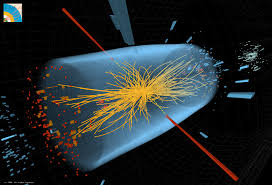
\includegraphics[height=0.6cm,width=0.8cm]{images/Intro/ppp.jpg}}
\end{picture}\put(10,2){\scriptsize\sf{Institut for theoretical physics}}\put(10,-2){\scriptsize\sf{Karlsruher institut for Technology (KIT)}}}
\cfoot{}
\rfoot{\footnotesize\sf{Thesis by Tigran Saidnia}}
\renewcommand{\headrulewidth}{0.4pt}
\renewcommand{\footrulewidth}{1.0pt}
\newcommand{\offline}{$ \overline{\textrm{\textbf{Off}}}\underline{\textrm{\textbf{line}}}\ $}


% ====================================================
% Kopf- und Fusszeile fuer "plain"-Format ueberschreiben
% ====================================================
\fancypagestyle{plain}{%
\fancyhf{}
\fancyfoot[L,C,R]{\setlength{\unitlength}{1mm}
\begin{picture}(0,0)
\put(0,-2){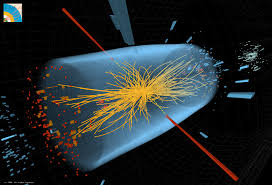
\includegraphics[height=0.6cm,width=0.8cm]{images/Intro/ppp.jpg}}
\end{picture}\put(10,2){\scriptsize\sf{Institut for theoretical physics}}\put(10,-2){\scriptsize\sf{Karlsruhe Institut of Technology (KIT)}}}
\cfoot{}
\rfoot{\footnotesize\sf{Thesis by Tigran Saidnia}}
\renewcommand{\headrulewidth}{0pt}
\renewcommand{\footrulewidth}{1.0pt}}

\begin{document}

%\doublespacing
    \parindent=0pt
    %\sloppypar
    \linespread{1.2}
    \thispagestyle{plain}
    %\frontmatter
    %\maketitle

\begin{titlepage}

\begin{center}


% Oberer Teil der Titelseite:

\includegraphics[width=0.3\textwidth]{images/Intro/kitlogo_de_rgb}\\[1cm]    

\textsc{\LARGE Master Thesis}\\[0.5cm]
\textsc{\Large by}\\[0.5cm]
\textsc{\Large Tigran Saidnia}\\[1.0cm]


% Title
\newcommand{\HRule}{\rule{\linewidth}{0.5mm}}
\HRule \\[0.8mm]
{\textbf{\Large \bfseries Emission kernels of parton showers in LO}}\\[0.8mm]

%\HRule \\[0.001mm]
%\newcommand{\HRule}{\rule{\linewidth}{0.5mm}}
%\HRule \\[0.8mm]
%{\textbf{\bfseries Emission kernels of parton showers in LO}}\\[0.8mm]

\HRule \\[1cm]
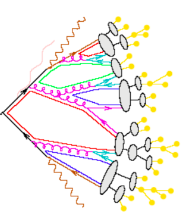
\includegraphics[scale=0.7]{images/Intro/footPicture.PNG}\\[0.8cm]   

\Large Karlsruhe institute of Technology (KIT)\\[1.5mm]
\Large Institute for theoretical physics\\[1.0cm]

{\Large Reviewer: PD Dr. Stefan Gieseke \\
\Large Second reviewer: Prof. Dr. Dieter Zeppenfeld\\
\Large External advisor: Dr. Simon Plätzer\\
\Large Advisor: Emma Simpson Dore}\\[0.8cm]   

Duration: July 1, 2018  –  July 1, 2019

\vfill

% Unterer Teil der Seite
 %\today

\end{center}

\end{titlepage}
\newpage
\chapter*{}
\begin{flushleft}
\vspace{11cm}
\textbf{Statement of Originality}\\[1cm]
I hereby confirm that I have written the accompanying thesis by myself, without contributions from any sources other than those cited in the text and acknowledgements. This applies also to all graphics, drawings, maps and images included in the thesis.\\[1cm]

Karlsruhe, \today \\[1cm]
\end{flushleft}

\begin{center}
---------------------------------\\
Tigran Saidnia
\end{center}

\pagebreak
\thispagestyle{empty}
\section*{\Large \bfseries \centering Abstract}
\vspace{1cm}
Infra red divergences come in two flavours:soft, due to the  massless  nature  of  the  radiation  (e.g.  the  massless photon in QED), and collinear, which comes from treating the radiating particle as massless.
By the Catani-Seymour dipole factorization a $m+1$-parton matrix element can be written as product of $m$-parton matrix element and an universal singular splitting function.  
In this work a mapping for $ 3\rightarrow 2 $ will be outlined and following along those lines one for $ m+1\rightarrow m $ is proposed, which is explicitly evaluated for the quadratic matrix elements in terms of the four possible parton splitting in the soft and collinear regions. Furthermore, a general prescription for the simplification of the usage of this algorithm in the next-to-leading order (NLO) level will also be given.  For comparison, the known result from the $ e^{+}e^{-} \rightarrow q \bar{q} g $ process is compared with the result of the gluon radiation from a parten quark in the first part of chapter \ref{LO}. 
The algorithm is straightforwardly implementable in general purpose \textup{Mathematica} or \textup{Herwig++} \cite{Bahr:2008pv}.

\vspace{3cm}
\section*{\Large \bfseries \centering Zusammenfassung}
\vspace{1cm}
Infrarot-Divergenzen gibt es in zwei Varianten: soft, aufgrund der massenlosen Natur der Emission (z.B. das massenlose Photon in QED), und kollinear, das von der Behandlung des strahlenden Partikels als massenlos verursacht wird.
Durch die Catani-Seymour Dipolfaktorisierung kann ein $m+1$-Partonmatrixelement als Produkt aus einem $m$-Parton Matrixelement und einer universellen singul\"aren Splittingfunktion geschrieben werden.  
In dieser Arbeit wird eine Mapping für $ 3\rightarrow 2 $ und ebenso f\"ur eine $ m+1\rightarrow m $ pr\"asentiert, die dann explizit bei der Auswertung der Matrixelemente der vier möglichen Partonsplittingen in den soft und kollinearen Bereichen eingesetzt wird. Vielmehr wird eine allgemeine Prozedur für die Vereinfachung dieses Algorithmusses in der Next-to-Leading Order (NLO) Ebene vorgeschlagen.  Zum Vergleich wird das bekannte Ergebnis aus $ e^{+}e^{-} \rightarrow q \bar{q} g $ Prozess mit dem Ergebnis der Gluonenabstrahlung eines Parent-Quarks aus dem ersten Teil vom Kapitel \ref{LO} verglichen. 
Der Algorithmus kann in \textup{Mathematica} oder \textup{Herwig++} \cite{Bahr:2008pv} implementiert werden.
\tableofcontents
\thispagestyle{empty}
\addcontentsline{toc}{chapter}{Table of contents}
\thispagestyle{empty}
\quad
\newpage
\pagenumbering{arabic}
\chapter*{Introduction}
\input{intro/intro.tex}




\newpage
\chapter{Theoretical Basics}
The Standard Model in particle physics encompasses all of the
Elementary particles and their interactions. It is a gauge theory spontaneously broken by the Higgs mechanism with the gauge group $ SU(3)_C \otimes SU(2)_L \otimes U(1)_Y $.\\
From a theoretical point of view, the Standard Model is a quantum field theory based on local gauge invariance and consists of two rough parts. The electroweak sector $ SU(2)_L \otimes U(1)_Y $ is called GWS (Glashow-Weinberg-Salam) theory and describes the gauge bosons $ W^{\pm}, Z^0, \gamma $, the Higgs sector and its interaction with the leptons and quarks. In contrast to the other gauge bosons, the exchange particles of the weak interaction carry mass, which also affects the properties of the interactions. The color-charged sector $ SU(3)_C $, the chromodynamics, deals with quarks and contains the eight massless, electrically neutral gluons as gauge bosons. The gauge groups $SU(3)_C$ and $SU(2)_L$ are non-abel gauge theories, more precisely Yang Mills theories.
The massive particles, fermions, will be divided into two groups, leptons and quarks. Each group is arranged in 3 generations. Within the leptons there are three electrically neutral neutrinos. The mass of the particles increases from generation to generation. Neutrinos only interact weakly, whereas the charged leptons interact both weakly and electromagnetically. Quarks are characterized by the fact that they can also interact strongly \cite{edelhaeuser2016tutorium}. 

\section{Quantum chromo dynamics}

Overall, there are four types of interactions.\\


\begin{tabular}{|c|c|c|c|c|}
\hline 
Interaction & Energy scale & Range [m] & Mediators \\ 
\hline 
Strong & $ \sim 1 $  & $10^{-15} $ & $g$ \\ 
\hline 
Electromagnetic & $ \sim 10^{-2} $ & $\infty$ & $\gamma $ \\ 
\hline  
Weak & $ \sim 10^{-6} $ & $10^{-18}$ & $W^{\pm}, Z$ \\ 
\hline
Gravity & $ \sim 10^{-38} $ & $\infty$ & maybe graviton \\ 
\hline 
\end{tabular}  
\\
\\
\\
Nucleons are made up of quark and gluons called partons.
Whereby, the gluons are the exchange bosons for this short ranged interaction.
\begin{figure}[h!]
\centering
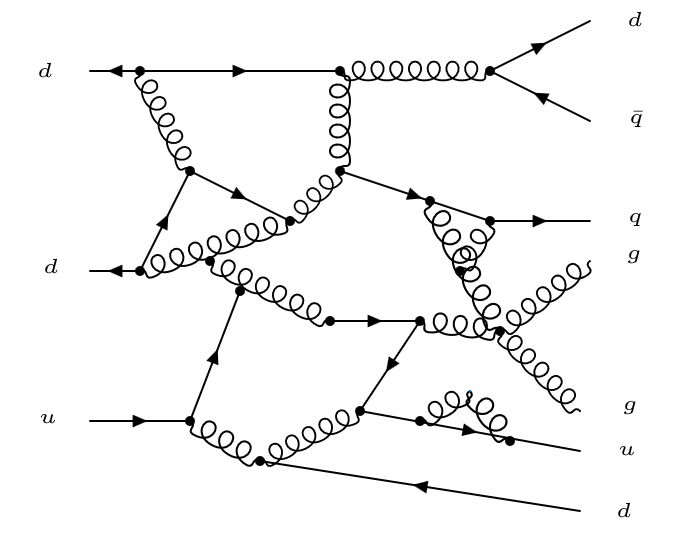
\includegraphics[scale=0.8]{images/Intro/Neutron.png}
\caption{A schematic picture of neutron structure. at the left side of the resolution is too low to see. The 3 quarks picture allows us to interpretate the quantum numbers of the neutron in the valence band.
In high-resolution picture for a large $ Q^2 $ can be obtained a gluon sea and a lot of quarks pairs\cite{Cunha13}. The quantum number of a neutron is for each energy scale the same}.
\end{figure}
To explain the short range of the strong interaction Yukawa (1934) postulated mesons as a mediator for the nuclear force by the exchange of this massive field quanta. Three years later a candidate ($ \pi $ meson) was found in cosmic rays. Later on it was shown massive field quanta break the gauge symmetry so that the mediator must be massless. If it is based on the SU(3) gauge symmetry of the QCD massless Lagrangian how can the strong sector be short range? Another question came from a series of experiments at SLAC. Through high-energy electron-proton scattering there was a search for evidence of the existence of quarks and their behaviour like free particles despite the energetically bound inner proton. The solution to these question was explained by Gross, Politzer and Wilczek through asymptotic freedom. 
This effect can be proved by the running coupling and anti screening in QCD.
For the calculation of the propagator loop correction in QCD both quark loops (negative contribution $ \rightarrow $ screening) and gluon loops (positive contribution $ \rightarrow $ anti screening) have to be taken into account. 
\begin{figure}[h!]
\centering
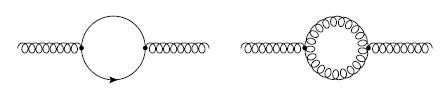
\includegraphics[scale=0.7]{images/Intro/quarkGluonPop.png}
\caption{Running coupling compared for QED, with a positive and QCD with a negative beta function. The quark loop vacuum polarization diagram gives a negative contribution
to $\beta_0 \sim n_f$ and the gluon loop gives a positive contribution to $\beta_0 \sim N_c$. The second contribution is bigger than the first, so that $ \beta_0 > 0 $ in QCD. The beta function in QED is negative since the second contribution does not exist $ N_C=0 $.}
\end{figure}

The one loop running coupling in QCD is:
\begin{equation}
\begin{split}
\alpha_s(Q^2)= \frac{\alpha_s(\mu^2)}{1+\beta_0 \alpha_s(\mu^2) ln(\frac{Q^2}{\mu^2})}
\end{split}
\end{equation}
\\
\\
\pagebreak

Where $ \beta_0 = \dfrac{11N_c -2n_f}{12\pi} $, $ n_f $ the number of quarks comes from the first diagram and causes screening.  $ N_c $ the number of colours is due to anti screening. Obviously, with $ n_f = 6 $ and $ N_c = 3 $ in standard model we will get $ \beta_0 >0 $. The Beta function is defined as:
\begin{equation}
\begin{split}
\beta(\alpha)=-(\beta_0 \alpha^2 + \beta_1 \alpha^3+\beta_2\alpha^4+....)=\frac{d\:\alpha(Q^2)}{d \:ln(Q^2)}
\end{split}
\end{equation}

e.g. the first term of beta-function is negative in contrast to QED with $ \beta_0=- \dfrac{\pi}{3} \rightarrow -(\beta_0 \alpha^2) >0 $. The coupling constant in QCD will be increased
with reduction of $ Q^2 $ (increasing distance), in QED vice versa.
\begin{figure}[h!]
\centering
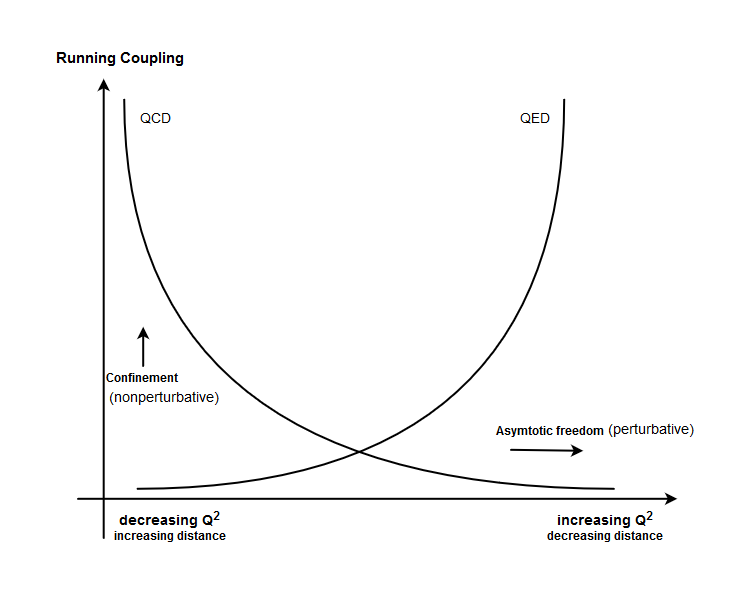
\includegraphics[scale=0.7]{images/Intro/QCDRunningCoupling.png}
\end{figure}



Asymptotic freedom allows us to use perturbation theory. Actually there is need of two more things to make the connection between theory and experiment: either infrared safety or factorisation. That is clarified in the next chapter\ref{Hard scattering}.
Quarks have not yet been observed as free particles. With increasing separation it will be easier to produce a quark-antiquark pair than to isolate a quark because the coupling between them is too strong. This mechanism is called confinement. Confinement as a non-perturbative theory has been confirmed in Lattice QCD, but not yet mathematically.
Quarks prefer to bind into hadrons which can be classified into baryons with three quarks state and mesons with a quark-antiquark state.
The wave function of fermions must be antisymmetric according to the Pauli exclusion principle under exchange of two quarks. Interestingly, there are resonance states with spin $ \frac{3}{2} $ like $ {\Delta}^{++} $.
The spins of the three up quarks are parallel to each other, have the same flavour and orbital angular momentum L=0. This means that an exchange of flavour, spin and space (orbital angular momentum) does not lead to any change. This problem was explained with the additional degree of freedom, the so-called color charge. This additional factor $N_C$ could be determined experimentally in the electron-positron annihilation into hadrons schematically in figure \ref{ratio}. 

\begin{figure}[h!]
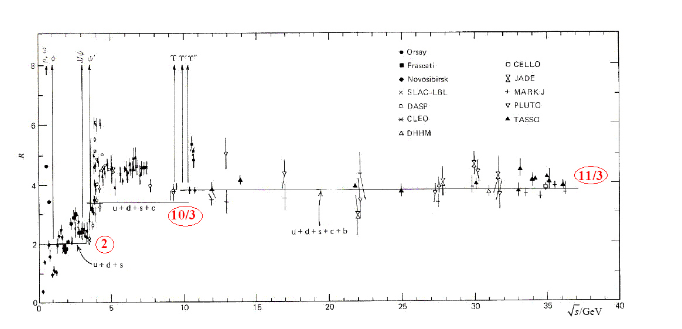
\includegraphics[width=1.1\textwidth, left]{images/Intro/Ratio.png}
\caption{Key measurement at lepton collider, $R = \frac{\sigma(e^+e^- \rightarrow Hadrons)}{\sigma(e^+e^- \rightarrow \mu^+ \mu^-)} =N_C \sum_q e^2_q$, evidence for $N_C=3$ colours of quarks. Without this factor the ration is for $ u, d, s $, $ u, d, s, c $ and $ u, d, s, c, b $ Respectively $ \frac{2}{3}, \frac{10}{9}, \frac{11}{10} $ The experiment showed a third of the expected results \cite{Eva}.}
\label{ratio}
\end{figure}


Each quark comes in one of three colours red, green or blue and also anti-colour $ \bar{r}, \bar{b}, \bar{g} $  for anti-quarks. The hadrons are colour singlets with regard to the hypothesis and so are invariant under rotations in colour space. The colour hypothesis describes the existence of mesons with $ q \bar{q} $ and baryons with $ qqq $. \\
The total wave function for each particle can be expressed:

\begin{equation}
\begin{split}
\Psi_{3q} &= \psi_{space} \times \chi_{spin} \times \theta_{colour} \times \phi_{flavour} \\
&\:\:\:\:\:\:\:O(3) \:\:\:\:\: SU(2)\:\:\:\: SU(3)\:\:\:\:\: SU(6)\\
\end{split}
\end{equation}
All possible colour states are described with Young Tableaux \cite{Greiner1989}. The group theory methods are used to decompose products of irreducible representations into sums for instance the Young Tableaux technique.
\begin{figure}[h!]
\centering
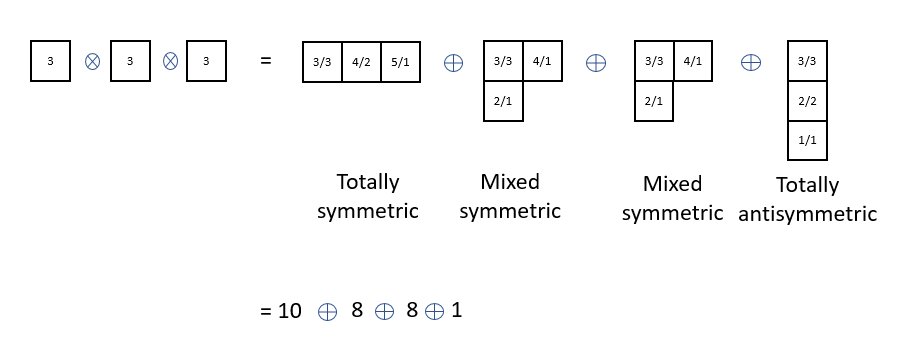
\includegraphics[scale=0.7]{images/Intro/Young.png}
\end{figure}

The same procedure for SU(2) and SU(6) for spins and flavours of the three quarks turns out:

\begin{equation}
\begin{split}
2\: \otimes\:2 \:\otimes\:2 &= 4 \:\:\:\oplus\: 2\:\:\:\oplus\:2\:\:\:\oplus\:0\\
6\: \otimes\:6 \:\otimes\:6&= 56 \:\oplus\: 70\:\oplus\:70\:\oplus\:20
\end{split}
\end{equation}


\pagebreak
\section{QCD Lagrangian}
\label{QCD Lagrangian}

QCD like QED and the weak interaction theory is described by representations of a symmetry group. From the condition that the Lagrangian must be invariant under arbitrary global and local symmetry transformations (Noether’s theorem) follows the interaction terms.
The Lagrangian of QCD is invariant under $ U(1) \times SU(3) $ global transformation. The three Pauli matrices from $ SU(2) $ can be replaced by the eight Gell-Mann $ \lambda^a $ with the following Lie algebra: 
\begin{equation}
\begin{split}
&T^a = \frac{1}{2} \lambda^a\\
&[T^a, T^b]= if^{abc} T^c \:\:\:\:\:\:\:\:\:\:\:\:\:\:\text{fundamental representation}\\
&({T^a}_{adj})_bc = -if^{abc} \:\:\:\:\:\:\:\:\:\:\:\:\text{adjoint representation}
\end{split}
\end{equation}
To quantize QCD theory, the Faddeev-Popov method \cite{Faddeev:1967fc} is usually used in the path integral to fix a gauge and define a gluon propagator. The Lagrangian is given:

\begin{equation}
\begin{split}
& \mathscr{L} = \sum_f \bar{\psi}_{if} (i\gamma^{\mu} {\partial}_{\mu}-m_f){\psi}^{jf}-\frac{1}{4}{F_a}^{\mu \nu}{F^a}_{\mu \nu}-\frac{1}{2\xi}(\partial^{\mu} {A^a}_{\mu})(\partial^{\nu} {A^a}_{\nu})+(\partial^{\mu} {\chi^a}^*)(\partial_{\mu} {\chi^a})\\
&{\color[RGB]{255,0,0} -g_s \bar{\psi}_{i} {T^a}_{ij}{\psi}_{j} \gamma^{\mu} {A^a}_{\mu}-\frac{g_s}{2} f^{abc}(\partial_{\mu} {A^a}_{\nu}-\partial_{\nu} {A^a}_{\mu}){A_b}^{\mu}{A_c}^{\nu})-\frac{{g_s}^2}{4} f^{abc} ({A_b}^{\mu}{A_c}^{\nu})f^{ade} ({A^d}_{\mu} {A^e}_{\nu})}\\
\\
&{\color[RGB]{255,0,0} -g_s f^{abc} (\partial^{\mu} {\chi^a}^{*}){\chi^b}{A^c}_{\mu}}\\
\end{split}
\end{equation}

The red marked part gives the Langrangian of free particles and the black part takes care of the interactions. ${F^a}_{\mu \nu}$ is field strength tensor for spin-1 gluon field $ {A^a}_{\mu} $ corresponded to a non-Abelian gauge theory with the structure constants $ f^{abc} $.

\begin{equation}
\begin{split}
{F^a}_{\mu \nu}= \partial_\mu {A^a}_{\nu}-\partial_\nu {A^a}_{\mu}-g_s f_{abc} {A^b}_{\mu} {A^c}_{\nu}
\end{split}
\end{equation}
The third term distinguishes QCD from QED, giving rise to triplet and quartic gluon self-interaction.
Here $i$, $j$ are color indices in the fundamental representation, $a, b , c$ run over 8 colour degrees of freedom of the gluon fields in the adjoint representation of SU(3). $f$ labels the six flavours of the quarks. $ g_s $ describes the strong coupling constant. Due to gauge fixing the Langrangian in the non-Abelian case requires the introduction of additional fields. These anti commuting complex scalar fields $ {\chi^a} $ are called Faddeev Popov ghosts \cite{Schwartz:2013pla, peskin2018introduction}. Feynman rules follows the Lagrangian. A list of the respective Feynman rules regarding the terms can be found in\ref{Math}  which will be used for the aims of this work later.

%
%\pagebreak
%It can be shown that the above Lagrangian is invariant under the following $ SU(3) $ gauge transformations:
%\begin{equation}
%\begin{split}
%&{\psi}^{\prime}(x) \rightarrow exp(i \:\eta_a(x) \:T^a) \:\psi(x)\\
%&{D}^{\prime} \rightarrow \partial_\mu+ig_sT_a\: {{A}^{\prime}}^a_{\mu } \\
%&{{A}^{\prime}}^a_{\mu }\rightarrow  {A^a}_{\mu}- \frac{1}{g_s}\partial_\mu \eta^a(x)+ f^{abc} \eta_{b}(x) {A_c}_{\nu}(x)
%\end{split}
%\end{equation}

\label{Feynman}

\pagebreak

\section{Colour factor calculation}
In this section the calculation of the Casimir operators of the respective diagrams is motivated, which occur later with the evaluation of the matrix elements. The generalization of the Pauli matrices are the so-called Gell-Mann matrices $\lambda ^a$ which is given by \cite{Schwartz:2013pla, Platzer:2018pmd}
\begin{equation}
\begin{split}
T^a = \vartheta^a \equiv \frac{\lambda ^2}{2}
\end{split}
\end{equation}

\begin{equation}
\begin{split}
\lambda ^1 =\begin{pmatrix} 0& 1 &\\ 1& 0 &\\ & & 0 \end{pmatrix},\:\:\: \lambda ^2 =\begin{pmatrix} 0& -i &\\ i& 0 &\\ & & 0 \end{pmatrix}, 
\:\:\: \lambda ^3 =\begin{pmatrix} 1&  &\\ & -1 &\\ & & 0 \end{pmatrix}, \:\:\: \lambda ^4 =\begin{pmatrix} &  &1\\ & 0&\\1 & &  \end{pmatrix}\\\
\lambda ^5 =\begin{pmatrix} &  &-i\\ & 0 &\\ i& &  \end{pmatrix},\:\:\: \lambda ^6 =\begin{pmatrix} 0&  &\\ & 0 &1\\ & 1& 0 \end{pmatrix}, 
\:\:\: \lambda ^7 =\begin{pmatrix} 0&  &\\ & 0 &-i\\ & i& 0 \end{pmatrix}, \:\:\: \lambda ^8 =\frac{1}{\sqrt3}\begin{pmatrix} 1&  &\\ & 1&\\ & &-2  \end{pmatrix}
\end{split}
\end{equation}
$ {\lambda}^3 $ and $  {\lambda}^8 $ are diagonal. These generators satisfy schematically:\\ 
\begin{itemize}
\item in the fundamental representation
\begin{figure}[h!]
\centering
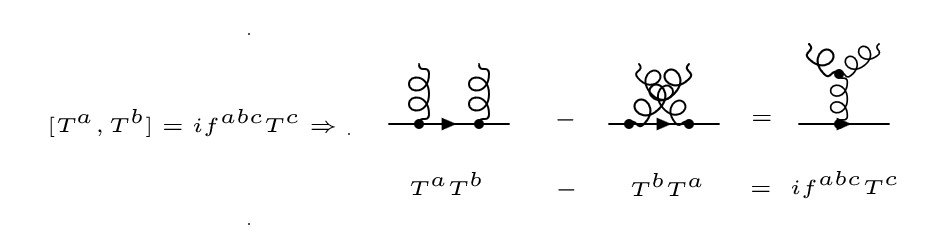
\includegraphics[scale=0.6]{images/Intro/Casimir.png}
\end{figure}
\item in the adjoint representation\\
\begin{figure}[h!]
\centering
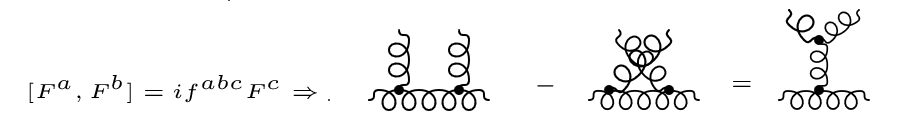
\includegraphics[scale=0.6]{images/Intro/CasimirAdj.png}
\end{figure}
\end{itemize}
\pagebreak
The most common convention for the normalization of the generators in physics is:
\begin{equation}
\displaystyle\sum\limits_{c,d} f^{acd} f^{bcd} = N \delta^{ab}
\end{equation}
One of the most important equations for the colour factor calculation is the Jaccobi-Identity:
\begin{equation}
\begin{split}\:
[T^a, [T^b , T^c]]+[T^c, [T^a , T^b]]+[T^b, [T^c , T^a]]=0
\end{split}
\end{equation}
In terms of the structure constant:
\begin{equation}
\begin{split}\:
f^{axd} f^{bcx} +  f^{cxd} f^{abx} +f^{bxd} f^{cax} =0
\end{split}
\end{equation}

\begin{equation}
f^{abc} = -2i\: tr(T^a[T^b, T^c])
\end{equation}
Which generalises to:
\begin{equation}
f^{abc}f^{xcd} = 4i\: tr(T^a[T^b, [T^c, T^d]])
\end{equation}

With these relations all Casimir operators can be calculated:\\
\begin{itemize}
\item Fundamental representation Casimir operator\\
\begin{figure}[h!]
\centering
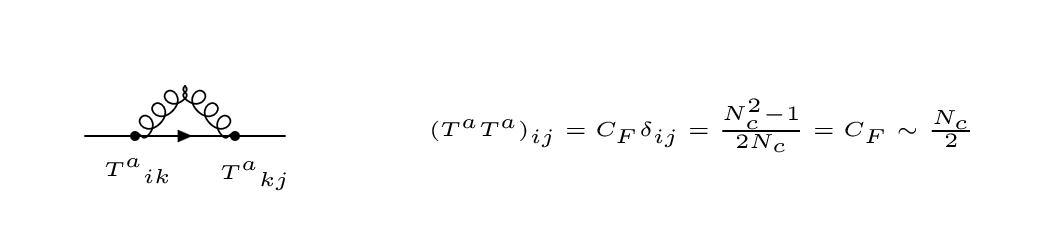
\includegraphics[scale=0.6]{images/Intro/Casimir1.png}
\end{figure}
\item Adjoint representation Casimir operator\\
\begin{figure}[h!]
\centering
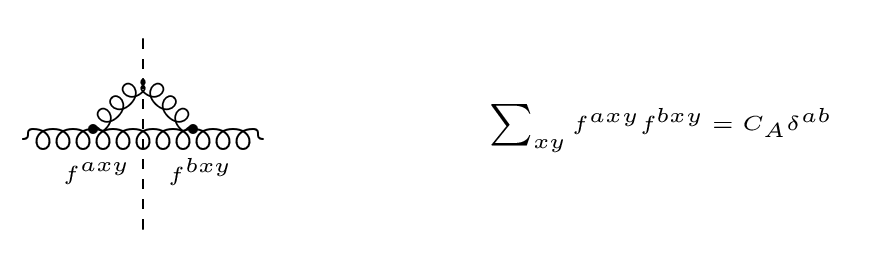
\includegraphics[scale=0.6]{images/Intro/Casimir2.png}
\end{figure}
\pagebreak
\\

Which means the charge of the gluon is twice that of the quark because:
\begin{equation}
 C_A = N_c =2C_F \sim 2(\frac{N_C}{2}) 
\end{equation}
\item Trace identities:\\
\begin{figure}[h!]
\centering
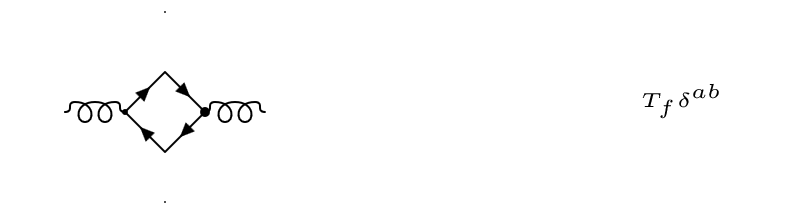
\includegraphics[scale=0.6]{images/Intro/Casimir3.png}
\end{figure}
\begin{figure}[h!]
\centering
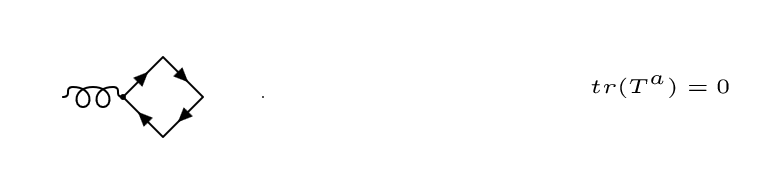
\includegraphics[scale=0.6]{images/Intro/Casimir4.png}
\end{figure}

\item Fierz identity
\end{itemize}
\begin{equation}
\displaystyle\sum\limits_{a} {T_{ij}}^a {T_{kl}}^a = \frac{1}{2}(\delta_{il}\delta_{kj}-\frac{1}{N}\delta_{ij}\delta_{kl})
\end{equation}
With this identity is clarified the difference between QED and QCD. The charge transfer in QED takes place along the Fermion line because photons cannot transport charges. On the other hand, the gluons transfer color charges. 
\begin{figure}[h!]
\centering
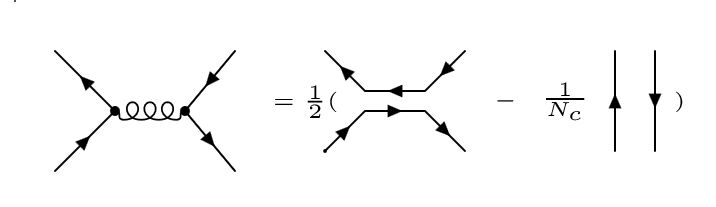
\includegraphics[scale=0.6]{images/Intro/Fritz.png}
\end{figure}
 

Other useful relation for the calculation of casimir operators in SU(N):
\begin{equation}
tr(T^a T^b)= {T_{ij}}^a {T_{ji}}^b = T_F \delta^{ab}
\end{equation}
\begin{equation}
\displaystyle\sum\limits_{a} (T^a T^a) = C_F \delta^{ij}
\end{equation}
\begin{equation}
f^{acd} f^{bcd} = C_A \delta^{ab}
\end{equation}
With $  T_F = \frac{1}{2} $ , $ C_A = N $ and $ C_F = \frac{N^2 -1}{2N} $



\newpage
\chapter{Catani Seymour}
\section{IR and Collinar Divergences}
Beyond the LO (Leading order) diagrams it happens singularities. To discuss about these consider first the process $ e^- e^+ \rightarrow q\bar{q}g $

\begin{figure}[ht!]
\centering
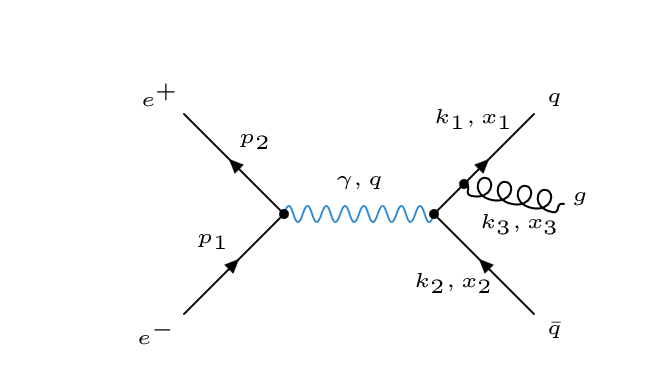
\includegraphics[width=0.85\textwidth]{images/Intro/IRCol.png}
\end{figure}
We define the energy fraction by:
\begin{equation}
x_i = \frac{2E_i}{\sqrt{s}}=\frac{2q\: \cdot\: k_i}{s}
\end{equation}
One can show that $ \sum x_i =2  $ and thus, that only two of the $ xi $ are independent.
In order to calculate the cross section of this diagram, we have to consider the gluon emission from the antiquark. Since the calculation is quite long, we concentrate on the final result, which can be found in almost every QCD lectures, e.g. H\&M Section 11.5.
\begin{figure}[ht!]
\centering
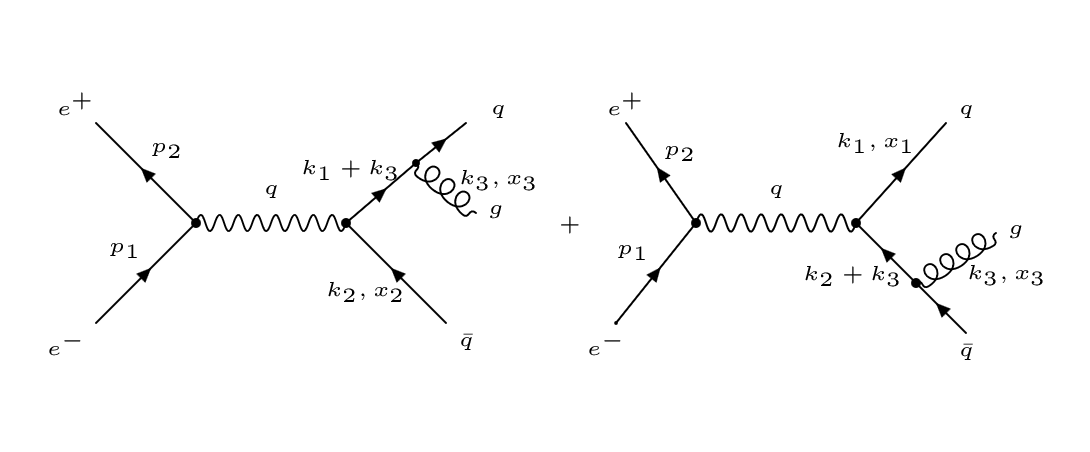
\includegraphics[width=0.85\textwidth]{images/Intro/IRColMatrix.png}
\caption{Left diagram $  e^- e^+ \rightarrow qg\bar{q} $ and right $ e^- e^+ \rightarrow q\bar{q}g $}
\end{figure}

The final result is:
\begin{equation}
\frac{d^2 \sigma}{dx_1 dx_2}= (\frac{4\pi \alpha}{s})\sum {e_i}^2 
\frac{2\alpha_s}{3\pi} \frac{{x_1}^2+{x_2}^2}{(1-x_1)(1-x_2)}
\end{equation}

There are three singularities in regard with the final result. 
If the emitted photon is collinear to the outgoing quark or anti-quark $ (x_1 \rightarrow 1 or x_2 \rightarrow 1) $ and When the emitted gluon is very soft $ (x_1 \rightarrow 1 and x_2 \rightarrow 1 )$.
The singularities come from the quark propagator in each diagram. The denominators contain according Feynmann rules terms with $\sim \frac{1}{(k_i + k_j)^2}  $. We can eliminate the quark mass under on-shell condition so that:
\begin{equation}
\frac{1}{(k_i + k_j)^2}=\frac{1}{2k_i \cdot k_j}=\frac{1}{2E_iE_j(1-cos\theta_{ij})}=\frac{1}{s(1- x_k)}
\end{equation} 
One can show all possibilities for three partons through a triangle:

\begin{figure}[ht!]
\centering
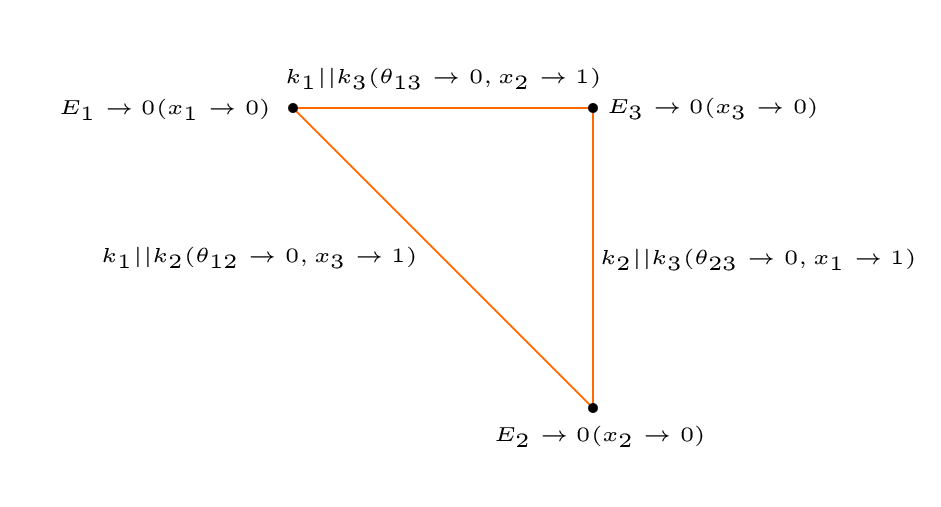
\includegraphics[width=0.85\textwidth]{images/Intro/triangle.png}
\end{figure}
We will use deep inelastic scattering (DIS) to show how the infrared singularities are absorbed in the parton distributions.
REAL and VIRT are separately divergent-could fix using splitting/subtraction method

\section{Factorisation}
The hadron hadron scattering can be written as:
\begin{equation}
\sigma = \sum_{ij} \int dx_1 dx_2 f_i(x_1, \mu^2)f_j(x_2, \mu^2) \sigma_{ij}(x_1, x_2, Q^2/\mu^2... )
\end{equation}
\begin{figure}[h!]
\centering
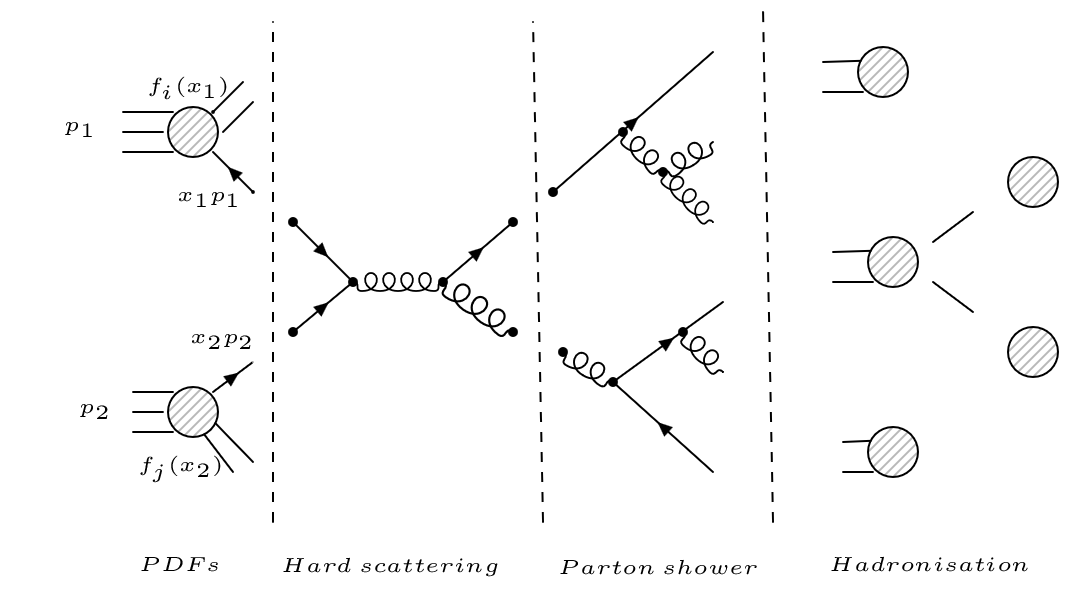
\includegraphics[width=0.85\textwidth]{images/Intro/Hard.png}
\end{figure}
Here the (arbitrary) factorisation scale $ \mu $ can be thought of
as the scale which separates the long and short-distance physics.
Roughly speaking, a parton with a transverse momentum less
than $ \mu $ is then considered to be part of the hadron structure and
is absorbed in the parton distribution. Partons with larger transverse
momenta participate in the hard scattering process with a
short-distance partonic cross-section.
The factorisation theorem also applies to deep inelastic scattering. The DIS cross section can be written as:
\begin{equation}
\frac{d^2 \sigma}{dx dQ^2}=\frac{4\pi \alpha^2}{x Q^4}[(1-y)F_2 (x, Q^2)+xy^2 F_1(x, Q^2)]
\end{equation}
In this case we need to introduce the structure function, is defined as the charge weighted sum of the parton momentum densities, the probability that the parton carries a momentum
fraction x. The index i denotes the quark. 
flavour.
\begin{equation}
{{F}_2}^{exp} (x)= \sum_i {e_i}^2 x f_i(x)
\end{equation}
The evolution of a quark
distribution due to gluon radiation and is called the DGLAP
evolution equation.
\begin{equation}
\frac{\partial f(x, \mu^2) }{\partial \: ln \:\mu^2}=
\frac{\alpha_s}{2\pi}\int_{x}^{1}\frac{dy}{y} f(y, \mu^2) P_{qq}(\frac{x}{y}+O({\alpha_s}^2)
\end{equation}
There three more spiriting possibilities according to below diagrams.

\begin{figure}[h!]
\centering
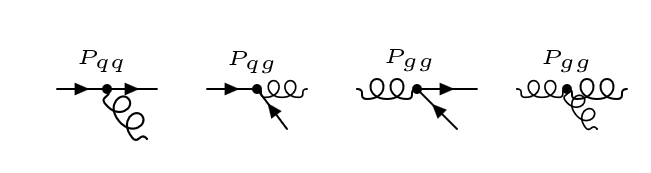
\includegraphics[width=0.85\textwidth]{images/Intro/spiliting.png}
\end{figure}

\begin{equation}
	\left.\begin{aligned}
\langle\:\hat{P_{qq}}\rangle &= C_F[\frac{1+z^2}{1-z}-\varepsilon(1-z)]\\
\langle\:\hat{P_{gq}}\rangle &= T_R[1-\frac{2z(1-z)}{1-\varepsilon}]\\
\langle\:\hat{P_{qg}}\rangle &= C_F[\frac{1+(1-z)^2}{z}-\varepsilon z]\\
\langle\:\hat{P_{gg}}\rangle &= 2C_A[\frac{z}{1-z}+\frac{1-z}{z}+z(1-z)]
\end{aligned}
	\right\}
	\quad \text{splitting functions}
\end{equation}

\section{splitting/subtraction method}

\section{Catani-Seymour Formalism}
\chapter{Analysis}
\section{Old parametrisation}

	
\begin{equation}
	\left.\begin{aligned}
	&{q_i}^{\mu} = z{p_i}^{\mu} + y(1-z){p_j}^{\mu} + \sqrt{zy(1-z)}{m}_{\bot} \\
	&{q}^{\mu}   = (1-z){p_i}^{\mu} + yz {p_j}^{\mu} - \sqrt{zy(1-z)}{m}_{\bot} \\
	&{q_j}^{\mu} = (1-y) {p_j}^{\mu} \\
		&y       = \frac{q_i q}{p_i p_j} \\
&q_i +q      = p_i + yp_j \\
&q_j +q      = (1-z){p_i}^{\mu} + (1+yz-y) {p_j}^{\mu} - \sqrt{zy(1-z)}{m}_{\bot}\\
&q_i \cdot q = y(1-2z+2z^2)(p_i \cdot p_j)\\
&q_i \cdot q_j = z(1-y) (p_i \cdot p_j)\\
&q_j \cdot q = (1-z)(1-y) (p_i \cdot p_j)
		\end{aligned}
	\right\}
	\quad \text{parametrisation}
\end{equation}


\section{new kinematic}
For the general m emission case it must be defined a new mapping. The parametrisation of the splitting momenta is formalized as:
\begin{equation}
	\begin{split}
	&{k_l}^{\mu} = \alpha_l \alpha {\Lambda^{\mu}}_{\nu}{p_i}^{\nu} + y\beta{n}^{\mu} + \sqrt{y\alpha_l\beta_l}{n^{\mu}}_{\bot,l} \:\:\:\:\:\:\:\:\:\:\:\:\:\:\:{l=1,...,m} \\
	&{q_i}^{\mu}   = (1-\displaystyle\sum\limits_{l=1}^m \alpha_l) \alpha {\Lambda^{\mu}}_{\nu}{p_i}^{\nu} + y(1-\displaystyle\sum\limits_{l=1}^m \beta_l){n}^{\mu} - \sqrt{y\alpha_l\beta_l}{n^{\mu}}_{\bot,l} \\
	&{q_k}^{\mu} = \alpha {\Lambda^{\mu}}_{\nu}{p_k}^{\nu} \:\:\:\:\:\:\:\:\:\:\:\:\: {k=1,...,n}\:\:\:\:\:\:\:\:\:\:k\neq i\\
    \end{split}
\end{equation}
$ k = 1,...,n $ labels the emission momenta and is taken to be massless $ {k_l}^2 = 0 $. Where the label $ l $ denotes the count of emissions. In this work we just want to considerate the one-emission kernels. The other important issue here is that all hard momenta are on-shell, $ {p_k}^2={q_k}^2=0 $.\\
to absorb the recoil we define $ n^{\mu} $ as:

\begin{equation}
\begin{split}
{n^{\mu}} &= Q^{\mu}-\frac{Q^2}{2p_i \cdot Q} {p_i}^{\mu}
\end{split}	
\end{equation}

Whereby Q is the total momentum with:

\begin{equation}
\begin{split}	
{Q}^{\mu} &= {q_i}^{\mu}+\displaystyle\sum\limits_{l=1}^m k_l^{\mu}+\displaystyle\sum\limits_{k=1}^m q_k^{\mu}={p_i}^{\mu}+\displaystyle\sum\limits_{k=1}^m p_k^{\mu}
\end{split}	
\end{equation}
To fulfil the condition that the emission momenta are massless, we need the following condition:

\begin{equation}
\begin{split}
	{n^{\mu}}_{\bot,l}{\Lambda^{\mu}}_{\nu}{p_i}^{\nu} &= {n_{\bot,l}} \cdot n = {n_{\bot,l}} \cdot Q =0\\
	{n^{\mu}}_{\bot,l}\cdot p_k &\neq0\\
\end{split}	
\end{equation}

$ {n}^2_{\bot,l} = -2\alpha{\Lambda^{\mu}}_{\nu}{p_i}^{\nu} n_{\mu} $ is not on-shell and in terms of single emission case we get $ {n}^2_{\bot,1} = -2p_i\cdot Q $.
The parameter y is related to the virtuality of the splitting parton:

\begin{equation}
\begin{split}
{q_i}^{\mu} +\displaystyle\sum\limits_{l=1}^m k_l^{\mu}   &= \alpha{\Lambda^{\mu}}_{\nu}{p_i}^{\nu} +y{n}^{\mu}\\
    \end{split}
\end{equation}
With $ \alpha = \sqrt{1-y} $.
\subsubsection*{Lorenz trafo}
In order to be able to work with the parametrisation, we have to do the Lorenz transformation of the Emitters, Spectator and total momentum first.

\begin{equation}
\begin{split}	
&\alpha{\Lambda^{\mu}}_{\nu} = {p_i}^{\mu} p_{i\nu} \frac{-y^2 Q^2}{4(p_i\cdot Q)^2(1+\sqrt{1-y}-\frac{y}{2})}
+{p_i}^{\mu} Q_{\nu} \frac{y(1+\sqrt{1-y})}{2(p_i\cdot Q)(1+\sqrt{1-y}-\frac{y}{2})}\\
&+{Q}^{\mu} p_{i\nu} \frac{(y^2 -y-y\sqrt{1-y})}{2(p_i\cdot Q)(1+\sqrt{1-y}-\frac{y}{2})}+\sqrt{1-y} {\eta^{\mu}}_{\nu}\\
\end{split}
\end{equation}

In the collinear limit of $ y \rightarrow 0, \alpha \rightarrow 1 $
this transformation reduces to trivial $ {\eta^{\mu}}_{\nu} $.


\begin{equation}
\begin{split}
&{\hat{{p_i}}}^{\mu}=\alpha{\Lambda^{\mu}}_{\nu} {p_i}^{\nu}= {p_i}^{\mu} p_{i\nu}{p_i}^{\nu} \frac{-y^2 Q^2}{4(p_i\cdot Q)^2(1+\sqrt{1-y}-\frac{y}{2})}
	+{p_i}^{\mu} Q_{\nu}{p_i}^{\nu} \frac{y(1+\sqrt{1-y})}{2(p_i\cdot Q)(1+\sqrt{1-y}-\frac{y}{2})}\\
&+{Q}^{\mu} p_{i\nu}{p_i}^{\nu} \frac{(y^2 -y-y\sqrt{1-y})}{2(p_i\cdot Q)(1+\sqrt{1-y}-\frac{y}{2})}+\sqrt{1-y} {\eta^{\mu}}_{\nu}{p_i}^{\nu}\\
\end{split}
\end{equation}

\begin{equation}
\begin{split}
&{\hat{{p_i}}}^{\mu}={p_i}^{\mu} (Q\cdot p_i) \frac{y(1+\sqrt{1-y})}{2(p_i\cdot Q)(1+\sqrt{1-y}-\frac{y}{2})}+\sqrt{1-y} {p_i}^{\mu}\\
&={p_i}^{\mu} [ \frac{y(1+\sqrt{1-y})}{(2+2\sqrt{1-y}-y)}+\sqrt{1-y}]={p_i}^{\mu}
    \end{split}
\end{equation}

\begin{equation}
	\begin{aligned}
		\fbox{$  {\hat{{p_i}}}^{\mu}=\alpha{\Lambda^{\mu}}_{\nu} {p_i}^{\nu}= {p_i}^{\mu}$}
    \end{aligned}
\end{equation}

\begin{equation}
	\begin{aligned}
	{\hat{{p_k}}}^{\mu}=\alpha{\Lambda^{\mu}}_{\nu} {p_k}^{\nu}= {p_i}^{\mu} p_{i\nu}{p_k}^{\nu} \frac{-y^2 Q^2}{4(p_i\cdot Q)^2(1+\sqrt{1-y}-\frac{y}{2})}
	+{p_i}^{\mu} Q_{\nu}{p_k}^{\nu} \frac{y(1+\sqrt{1-y})}{2(p_i\cdot Q)(1+\sqrt{1-y}-\frac{y}{2})}\\
	+{Q}^{\mu} p_{i\nu}{p_k}^{\nu} \frac{(y^2 -y-y\sqrt{1-y})}{2(p_i\cdot Q)(1+\sqrt{1-y}-\frac{y}{2})}+\sqrt{1-y} {\eta^{\mu}}_{\nu}{p_k}^{\nu}\\
    \end{aligned}
\end{equation}

\begin{equation}
	\begin{aligned}
	{\hat{{p_k}}}^{\mu}=\alpha{\Lambda^{\mu}}_{\nu} {p_k}^{\nu}= {p_i}^{\mu}[  \frac{-y^2 Q^2 (p_{i}\cdot {p_k})}{4(p_i\cdot Q)^2(1+\sqrt{1-y}-\frac{y}{2})}+ \frac{y(1+\sqrt{1-y})(Q \cdot {p_k})}{2(p_i\cdot Q)(1+\sqrt{1-y}-\frac{y}{2})}]\\
	+{Q}^{\mu} [ \frac{(y^2 -y-y\sqrt{1-y}) (p_{i}\cdot {p_k})}{2(p_i\cdot Q)(1+\sqrt{1-y}-\frac{y}{2})}]
	+\sqrt{1-y} {p_k}^{\mu}\\
    \end{aligned}
\end{equation}


\begin{equation}
	\begin{aligned}
	{\hat{{p_k}}}^{\mu}&=\alpha{\Lambda^{\mu}}_{\nu} {p_k}^{\nu}= {p_i}^{\mu}[  \frac{-y^2 Q^2 (p_{i}\cdot {p_k})}{4(p_i\cdot Q)^2(1+\sqrt{1-y}-\frac{y}{2})}+ \frac{y(1+\sqrt{1-y})(Q \cdot {p_k})}{2(p_i\cdot Q)(1+\sqrt{1-y}-\frac{y}{2})}]\\
	&+{Q}^{\mu} [ \frac{(y^2 -y-y\sqrt{1-y}) (p_{i}\cdot {p_k})}{2(p_i\cdot Q)(1+\sqrt{1-y}-\frac{y}{2})}]+\sqrt{1-y} {p_k}^{\mu}\\	
\text{with}\\
	A_1 &\equiv  \frac{-y^2 Q^2 (p_{i}\cdot {p_k})}{4(p_i\cdot Q)^2(1+\sqrt{1-y}-\frac{y}{2})}+ \frac{y(1+\sqrt{1-y})(Q \cdot {p_k})}{2(p_i\cdot Q)(1+\sqrt{1-y}-\frac{y}{2})}\\
		A_2 &\equiv   \frac{(y^2 -y-y\sqrt{1-y}) (p_{i}\cdot {p_k})}{2(p_i\cdot Q)(1+\sqrt{1-y}-\frac{y}{2})}\:\:\:\:\:\:\:\:\:\:\:\:\:\:\:\:\:\:\:\:\:\:\:\:\:\:\:\:\:\:\:\:\:\:\:\:\:\:\:\:\:\:\:\:\:\:\:\:\:\:\:\:\:\:\\\
    \end{aligned}    
\end{equation}
\begin{equation}
	\begin{aligned}
		\fbox{$  {\hat{{p_k}}}^{\mu}= A_1 \:{p_i}^{\mu}+A_2\:{Q}^{\mu}+\sqrt{1-y} {p_k}^{\mu} $}
    \end{aligned}
\end{equation}


\begin{equation}
	\begin{aligned}
	{\hat{{Q}}}^{\mu}&=\alpha{\Lambda^{\mu}}_{\nu} {Q}^{\nu}= {p_i}^{\mu}[  \frac{-y^2 Q^2 (p_{i}\cdot {Q})}{4(p_i\cdot Q)^2(1+\sqrt{1-y}-\frac{y}{2})}+ \frac{y(1+\sqrt{1-y})Q^2}{2(p_i\cdot Q)(1+\sqrt{1-y}-\frac{y}{2})}]\\
	&+{Q}^{\mu} [ \frac{(y^2 -y-y\sqrt{1-y}) (p_{i}\cdot {Q})}{2(p_i\cdot Q)(1+\sqrt{1-y}-\frac{y}{2})}]
	+\sqrt{1-y} {Q}^{\mu}\\
\text{with}\\
	S_1 &\equiv  \frac{Q^2}{2p_i \cdot Q}[\frac{-y^2}{2(1+\sqrt{1-y}-\frac{y}{2})}+ \frac{y(1+\sqrt{1-y})}{(1+\sqrt{1-y}-\frac{y}{2})}]=\frac{Q^2}{2p_i \cdot Q}y\\
		S_2 &\equiv   \frac{(y^2 -y-y\sqrt{1-y})}{2(1+\sqrt{1-y}-\frac{y}{2})}+\sqrt{1-y}=1-y\:\:\:\:\:\:\:\:\:\:\:\:\:\:\:\:\:\:\:\:\:\:\:\:\:\:\:\:\:\:\:\:\:\:\:\:\:\:\:\:\:\:\:\:\:\:\:\:\:\:\:\:\:\:\\\	
    \end{aligned}    
\end{equation}
\begin{equation}
	\begin{aligned}
		\fbox{$  {\hat{{Q}}}^{\mu}= \frac{Q^2}{2p_i \cdot Q}y \:{p_i}^{\mu}+(1-y)\:{Q}^{\mu} $}
    \end{aligned}
\end{equation}

\section{Single emission part}
\begin{equation}
	\begin{aligned}
	{k_1}^{\mu} &= (\alpha_1 -y\beta_1(\frac{Q^2}{2p_i \cdot Q})) {p_i}^{\mu} + y\beta_1{Q}^{\mu} + \sqrt{y\alpha_1\beta_1}{n^{\mu}}_{\bot,1}  \\
	{q_i}^{\mu}   &= (\beta_1 -\alpha_1 y(\frac{Q^2}{2p_i \cdot Q})){p_i}^{\mu} + y\alpha_1{Q}^{\mu} - \sqrt{y\alpha_1\beta_1}{n^{\mu}}_{\bot,l} \\
	{q_k}^{\mu} &= \alpha {\Lambda^{\mu}}_{\nu}{p_k}^{\nu} \:\:\:\:\:\:\:\:\:\:\:\:\: {k=1,...,n}\:\:\:\:\:\:\:\:\:\:k\neq i\\
	\\
	\\
		{k_1}^{\mu} &= \zeta_1 {p_i}^{\mu} + \lambda_1{Q}^{\mu} + \sqrt{y\alpha_1\beta_1}{n^{\mu}}_{\bot,1}  \\
	{q_i}^{\mu}   &= \zeta_q{p_i}^{\mu} + \lambda_q{Q}^{\mu} - \sqrt{y\alpha_1\beta_1}{n^{\mu}}_{\bot,l} \\
	{q_k}^{\mu} &= A_1{p_i}^{\mu} + A_2{Q}^{\mu} + \sqrt{1-y}{p_k^{\mu}}\\
    \end{aligned}
\end{equation}

\begin{equation}
	\begin{aligned}
	\zeta_1\zeta_1=({\alpha_1}^2 -2y\alpha_1 \beta_1(\frac{Q^2}{2p_i \cdot Q})+y^2{\beta_1}^2(\frac{Q^2}{2p_i \cdot Q})^2)\\
	\zeta_1\lambda_1=(y\alpha_1\beta_1 -{y^2\beta_1}^2(\frac{Q^2}{2p_i \cdot Q}))\\
	\zeta_1\zeta_q=(\alpha_1\beta_1-y({\alpha_1}^2+{\beta_1}^2) (\frac{Q^2}{2p_i \cdot Q})+y^2{\alpha_1}{\beta_1}(\frac{Q^2}{2p_i \cdot Q})^2)\\
	\zeta_1\lambda_q=(y{\alpha_1}^2 -y^2\beta_1\alpha_1(\frac{Q^2}{2p_i \cdot Q}))\\
	\zeta_q\zeta_q=	({\beta_1}^2 -2y\alpha_1\beta_1 (\frac{Q^2}{2p_i \cdot Q})+ y^2{\alpha_1}^2 (\frac{Q^2}{2p_i \cdot Q})^2) \\
	\zeta_q\lambda_1=(y{\beta_1}^2 -y^2\alpha_1 \beta_1(\frac{Q^2}{2p_i \cdot Q}))\\
	\zeta_q\zeta_1=(\beta_1\alpha_1-y({\beta_1}^2+{\alpha_1}^2)(\frac{Q^2}{2p_i \cdot Q})+y^2\alpha_1\beta_1 (\frac{Q^2}{2p_i \cdot Q})^2)\\
	\zeta_q\lambda_q=(y\beta_1\alpha_1 -y^2{\alpha_1}^2(\frac{Q^2}{2p_i \cdot Q}))\\
	\lambda_1\lambda_1=y^2{\beta_1}^2\\
	\lambda_1\zeta_q=(y{\beta_1}^2 -y^2\alpha_1 \beta_1(\frac{Q^2}{2p_i \cdot Q}))\\
	\lambda_1\lambda_q=y^2\beta_1\alpha_1\\
	\lambda_1\zeta_1=(y\beta_1\alpha_1 -y^2{\beta_1}^2(\frac{Q^2}{2p_i \cdot Q}))\\
	\lambda_q\lambda_q=y^2{\alpha_1}^2\\
	\lambda_q\lambda_1=y^2\alpha_1\beta_1\\
	\lambda_q\zeta_q=(y\alpha_1\beta_1 -y^2{\alpha_1}^2 (\frac{Q^2}{2p_i \cdot Q}))\\
	\lambda_q\zeta_1=(y{\alpha_1}^2 -y^2\alpha_1\beta_1(\frac{Q^2}{2p_i \cdot Q}))
    \end{aligned}
\end{equation}
\section{Common scalar products}
\begin{equation}
	\begin{aligned}	
k_1 \cdot q_i &= (\zeta_1 \lambda_q + \lambda_1 \zeta_q)p_i \cdot Q+\lambda_1 \lambda_q Q^2 -y\alpha_1\beta_1 {n^{2}}_{\bot,1}\\
	&=[(\alpha_1 -y\beta_1(\frac{Q^2}{2p_i \cdot Q}))y\alpha_1+y\beta_1(\beta_1 -\alpha_1 y(\frac{Q^2}{2p_i \cdot Q}))]\:p_i \cdot Q\\
	&\:\:\:\:\:\:\:y^2\beta_1\alpha_1\: Q^2+2y\alpha_1\beta_1\:p_iQ\\
\Rightarrow	k_1 \cdot q_i &=[y{\alpha_1}^2 -y^2\alpha_1\beta_1(\frac{Q^2}{2p_i \cdot Q})+y {\beta_1}^2-y^2\alpha_1\beta_1(\frac{Q^2}{2p_i \cdot Q})]\:p_i\cdot Q\\
	&y^2\beta_1\alpha_1\: Q^2+2y\alpha_1\beta_1\:p_iQ\\	
    \end{aligned}
\end{equation}

\begin{equation}
	\begin{aligned}
		\fbox{$  k_1 \cdot q_i=y({\alpha_1}+\beta_1)^2\:p_i\cdot Q = y\:p_i\cdot Q $}
    \end{aligned}
\end{equation}

\begin{equation}
	\begin{aligned}	
	k_1 \cdot q_k &= (\zeta_1 A_2 + \lambda_1 A_1)p_i \cdot Q+\zeta_1 \sqrt{1-y}\:p_i\cdot p_k + \lambda_1 A_2\:Q^2+ \lambda_1\sqrt{1-y}\:Q\cdot p_k\\
	&+\sqrt{\alpha_1\beta_1y(1-y)} p_k \cdot {n_{\bot,1}}\\	
	&=\lbrace[(\alpha_1 -y\beta_1(\frac{Q^2}{2p_i \cdot Q}))\frac{(y^2 -y-y\sqrt{1-y}) (p_{i}\cdot {p_k})}{2(p_i\cdot Q)(1+\sqrt{1-y}-\frac{y}{2})}]\\&
	+y\beta_1[\frac{-y^2 Q^2 (p_{i}\cdot {p_k})}{4(p_i\cdot Q)^2(1+\sqrt{1-y}-\frac{y}{2})}+ \frac{y(1+\sqrt{1-y})(Q \cdot {p_k})}{2(p_i\cdot Q)(1+\sqrt{1-y}-\frac{y}{2})}]\rbrace\:p_i \cdot Q\\
	&+(\alpha_1 -y\beta_1(\frac{Q^2}{2p_i \cdot Q}))\sqrt{1-y}\:p_i \cdot p_k+y\beta_1\frac{(y^2 -y-y\sqrt{1-y}) (p_{i}\cdot {p_k})}{2(p_i\cdot Q)(1+\sqrt{1-y}-\frac{y}{2})}Q^2\\
	&+y\beta_1\sqrt{1-y} Q\cdot p_k+\sqrt{\alpha_1\beta_1y(1-y)} p_k \cdot {n_{\bot,1}} 
    \end{aligned}
\end{equation}

\begin{equation}
	\begin{aligned}
	k_1 \cdot q_k &= \alpha_1 \frac{(y^2 -y-y\sqrt{1-y}) }{2(1+\sqrt{1-y}-\frac{y}{2})}(p_{i}\cdot {p_k})
	-y\beta_1(\frac{Q^2}{2p_i \cdot Q})\frac{(y^2 -y-y\sqrt{1-y})}{2(1+\sqrt{1-y}-\frac{y}{2})}(p_{i}\cdot {p_k})\\
&+y\beta_1\frac{-y^2 Q^2 }{4(p_i\cdot Q)(1+\sqrt{1-y}-\frac{y}{2})}(p_{i}\cdot {p_k})+ y\beta_1\frac{y(1+\sqrt{1-y})}{2(1+\sqrt{1-y}-\frac{y}{2})}\:Q \cdot p_k\\
	&+\alpha_1 \sqrt{1-y}\:p_i \cdot p_k-y\beta_1(\frac{Q^2}{2p_i \cdot Q})\sqrt{1-y}\:p_i \cdot p_k\\
	&+y\beta_1(\frac{Q^2}{2p_i \cdot Q})\frac{(y^2 -y-y\sqrt{1-y})}{2(1+\sqrt{1-y}-\frac{y}{2})}(p_{i}\cdot {p_k})+y\beta_1\sqrt{1-y}(Q\cdot p_k)\\
	&+\sqrt{\alpha_1\beta_1y(1-y)} p_k \cdot {n_{\bot,1}} 
    \end{aligned}
\end{equation}

\begin{equation}
	\begin{aligned}
	k_1 \cdot q_k &= [\alpha_1 \frac{(y^2 -y-y\sqrt{1-y}) }{2(1+\sqrt{1-y}-\frac{y}{2})}+y\beta_1\frac{-y^2 Q^2 }{4(p_i\cdot Q)(1+\sqrt{1-y}-\frac{y}{2})}+\alpha_1 \sqrt{1-y}\\&-y\beta_1(\frac{Q^2}{2p_i \cdot Q})\sqrt{1-y}]\:p_i \cdot p_k+[y\beta_1\frac{y(1+\sqrt{1-y})}{2(1+\sqrt{1-y}-\frac{y}{2})}+y\beta_1\sqrt{1-y}](Q\cdot p_k)\\
	&+\sqrt{\alpha_1\beta_1y(1-y)} p_k \cdot {n_{\bot,1}} 
    \end{aligned}
\end{equation}

\begin{equation}
	\begin{aligned}
	k_1 \cdot q_k &= \lbrace\alpha_1 [\frac{(y^2 -y-y\sqrt{1-y}) }{2(1+\sqrt{1-y}-\frac{y}{2})}+ \sqrt{1-y}]\\
	&+y\beta_1(\frac{Q^2}{p_i \cdot Q})[\frac{-y^2 }{4(1+\sqrt{1-y}-\frac{y}{2})}-\sqrt{1-y}]\rbrace\:p_i \cdot p_k\\
	&+y\beta_1[\frac{y(1+\sqrt{1-y})}{2(1+\sqrt{1-y}-\frac{y}{2})}+\sqrt{1-y}](Q\cdot p_k)\\
	&+\sqrt{\alpha_1\beta_1y(1-y)} p_k \cdot {n_{\bot,1}} 
    \end{aligned}
\end{equation}

\begin{equation}
	\begin{aligned}
		\fbox{$  k_1 \cdot q_k = [\alpha_1 (1-y)+y\beta_1(\frac{Q^2}{2p_i \cdot Q})]\:p_i \cdot p_k+y\beta_1\:Q\cdot p_k+\sqrt{\alpha_1\beta_1y(1-y)} p_k \cdot {n_{\bot,1}} $}
    \end{aligned}
\end{equation}

\begin{equation}
	\begin{aligned}	
	q_i \cdot q_k &= (\zeta_q A_2 + \lambda_q A_1)p_i \cdot Q+\zeta_q \sqrt{1-y}\:p_i\cdot p_k + \lambda_q A_2\:Q^2+ \lambda_q\sqrt{1-y}\:Q\cdot p_k\\
	&-\sqrt{\alpha_1\beta_1y(1-y)} p_k \cdot {n_{\bot,1}}\\	
	&=\lbrace[(\beta_1 -y\alpha_1(\frac{Q^2}{2p_i \cdot Q}))\frac{(y^2 -y-y\sqrt{1-y}) (p_{i}\cdot {p_k})}{2(p_i\cdot Q)(1+\sqrt{1-y}-\frac{y}{2})}]\\&
	+y\alpha_1[\frac{-y^2 Q^2 (p_{i}\cdot {p_k})}{4(p_i\cdot Q)^2(1+\sqrt{1-y}-\frac{y}{2})}+ \frac{y(1+\sqrt{1-y})(Q \cdot {p_k})}{2(p_i\cdot Q)(1+\sqrt{1-y}-\frac{y}{2})}]\rbrace\:p_i \cdot Q\\
	&+(\beta_1 -y\alpha_1(\frac{Q^2}{2p_i \cdot Q}))\sqrt{1-y}\:p_i \cdot p_k+y\alpha_1\frac{(y^2 -y-y\sqrt{1-y}) (p_{i}\cdot {p_k})}{2(p_i\cdot Q)(1+\sqrt{1-y}-\frac{y}{2})}Q^2\\
	&+y\alpha_1\sqrt{1-y} Q\cdot p_k-\sqrt{\alpha_1\beta_1y(1-y)} p_k \cdot {n_{\bot,1}} 
    \end{aligned}
\end{equation}


\begin{equation}
	\begin{aligned}
	q_i \cdot q_k &= \beta_1 \frac{(y^2 -y-y\sqrt{1-y}) }{2(1+\sqrt{1-y}-\frac{y}{2})}(p_{i}\cdot {p_k})
	-y\alpha_1(\frac{Q^2}{2p_i \cdot Q})\frac{(y^2 -y-y\sqrt{1-y})}{2(1+\sqrt{1-y}-\frac{y}{2})}(p_{i}\cdot {p_k})\\
&+y\alpha_1\frac{-y^2 Q^2 }{4(p_i\cdot Q)(1+\sqrt{1-y}-\frac{y}{2})}(p_{i}\cdot {p_k})+ y\alpha_1\frac{y(1+\sqrt{1-y})}{2(1+\sqrt{1-y}-\frac{y}{2})}\:Q \cdot p_k\\
	&+\beta_1 \sqrt{1-y}\:p_i \cdot p_k-y\alpha_1(\frac{Q^2}{2p_i \cdot Q})\sqrt{1-y}\:p_i \cdot p_k\\
	&+y\alpha_1(\frac{Q^2}{2p_i \cdot Q})\frac{(y^2 -y-y\sqrt{1-y})}{2(1+\sqrt{1-y}-\frac{y}{2})}(p_{i}\cdot {p_k})+y\alpha_1\sqrt{1-y}(Q\cdot p_k)\\
	&-\sqrt{\alpha_1\beta_1y(1-y)} p_k \cdot {n_{\bot,1}} 
    \end{aligned}
\end{equation}

\begin{equation}
	\begin{aligned}
	q_i \cdot q_k &= [\beta_1 \frac{(y^2 -y-y\sqrt{1-y}) }{2(1+\sqrt{1-y}-\frac{y}{2})}+y\alpha_1\frac{-y^2 Q^2 }{4(p_i\cdot Q)(1+\sqrt{1-y}-\frac{y}{2})}+\beta_1 \sqrt{1-y}\\&-y\alpha_1(\frac{Q^2}{2p_i \cdot Q})\sqrt{1-y}]\:p_i \cdot p_k+[y\alpha_1\frac{y(1+\sqrt{1-y})}{2(1+\sqrt{1-y}-\frac{y}{2})}+y\alpha_1\sqrt{1-y}](Q\cdot p_k)\\
	&-\sqrt{\alpha_1\beta_1y(1-y)} p_k \cdot {n_{\bot,1}} 
    \end{aligned}
\end{equation}

\begin{equation}
	\begin{aligned}
	k_1 \cdot q_k &= \lbrace\beta_1 [\frac{(y^2 -y-y\sqrt{1-y}) }{2(1+\sqrt{1-y}-\frac{y}{2})}+ \sqrt{1-y}]\\
	&+y\alpha_1(\frac{Q^2}{p_i \cdot Q})[\frac{-y^2 }{4(1+\sqrt{1-y}-\frac{y}{2})}-\sqrt{1-y}]\rbrace\:p_i \cdot p_k\\
	&+y\alpha_1[\frac{y(1+\sqrt{1-y})}{2(1+\sqrt{1-y}-\frac{y}{2})}+\sqrt{1-y}](Q\cdot p_k)\\
	&-\sqrt{\alpha_1\beta_1y(1-y)} p_k \cdot {n_{\bot,1}} 
    \end{aligned}
\end{equation}

\begin{equation}
	\begin{aligned}
		\fbox{$  q_i \cdot q_k = [\beta_1 (1-y)+y\alpha_1(\frac{Q^2}{2p_i \cdot Q})]\:p_i \cdot p_k+y\alpha_1\:Q\cdot p_k-\sqrt{\alpha_1\beta_1y(1-y)} p_k \cdot {n_{\bot,1}} $}
    \end{aligned}
\end{equation}

\section{Parametrization in terms of $ (k_1 \cdot q_i )(k_1 \cdot q_k) $}
\begin{equation}
	\begin{aligned}
		\fbox{$  (k_1 \cdot q_i )(k_1 \cdot q_k) {\color[RGB]{255,0,0} \: \approx\:} y(1-\beta_1) (1-y)\:(p_i \cdot p_k)(p_i \cdot Q) $}
    \end{aligned}
\end{equation}

\begin{equation}
\begin{split}
{k_1}^{{\eta}}{k_1}^{{\eta}^{\prime}}&=[(1-\beta_1)^2-y^2 {\beta_1}^2 (\frac{Q^2}{2p_i \cdot Q})^2] {p_i}^{{\eta}}{p_i}^{{\eta}^{\prime}}-y^2 {\beta_1}^2 (\frac{Q^2}{2p_i \cdot Q}){p_i}^{{\eta}}{Q}^{{\eta}^{\prime}}-y^2 {\beta_1}^2 (\frac{Q^2}{2p_i \cdot Q}){Q}^{{\eta}}{p_i}^{{\eta}^{\prime}}\\
{k_1}^{{\eta}}{q_i}^{{\eta}^{\prime}}&=[\beta_1(1-\beta_1)-y {\beta_1}^2 (\frac{Q^2}{2p_i \cdot Q})] {p_i}^{{\eta}}{p_i}^{{\eta}^{\prime}}+y {\beta_1}^2 {Q}^{{\eta}}{p_i}^{{\eta}^{\prime}}\\
{q_i}^{{\eta}}{k_1}^{{\eta}^{\prime}}&=[\beta_1(1-\beta_1)-y {\beta_1}^2 (\frac{Q^2}{2p_i \cdot Q})] {p_i}^{{\eta}}{p_i}^{{\eta}^{\prime}}+y {\beta_1}^2 {p_i}^{{\eta}}{Q}^{{\eta}^{\prime}}\\
{q_i}^{{\eta}}{q_i}^{{\eta}^{\prime}}&={\beta_1}^2 {p_i}^{{\eta}}{p_i}^{{\eta}^{\prime}}\\
{k_1}^{{\eta}}{q_k}^{{\eta}^{\prime}}&= [(1-\beta_1)-y\beta_1 (\frac{Q^2}{2p_i \cdot Q})] \sqrt{1-y}{p_i}^{{\eta}}{{p_k}^{{\eta}^{\prime}}}-y {\beta_1} (\frac{Q^2}{2p_i \cdot Q}) A_1 \:{p_i}^{{\eta}}{p_i}^{{\eta}^{\prime}}
-y {\beta_1} (\frac{Q^2}{2p_i \cdot Q}) A_2\: {p_i}^{{\eta}}{Q}^{{\eta}^{\prime}}\\
&+y {\beta_1} A_1 \:{Q}^{{\eta}}{p_i}^{{\eta}^{\prime}}+y {\beta_1} A_2 \:{Q}^{{\eta}}{Q}^{{\eta}^{\prime}}+y {\beta_1}\sqrt{1-y}{Q}^{{\eta}}{{p_k}^{{\eta}^{\prime}}}\\
{q_i}^{{\eta}}{q_k}^{{\eta}^{\prime}}&=A_1\beta_1 {p_i}^{{\eta}}{{p_i}^{{\eta}^{\prime}}}+A_2\beta_1 {p_i}^{{\eta}}{{Q}^{{\eta}^{\prime}}}+\beta_1 \sqrt{1-y}{p_i}^{{\eta}}{{p_k}^{{\eta}^{\prime}}}\\
{q_k}^{\eta}{k_1}^{{{\eta}}^{\prime}}&=[(1-\beta_1)-y\beta_1 (\frac{Q^2}{2p_i \cdot Q})] \sqrt{1-y}{p_k}^{{\eta}}{{p_i}^{{\eta}^{\prime}}}-y {\beta_1} (\frac{Q^2}{2p_i \cdot Q}) A_1 \:{p_i}^{{\eta}}{p_i}^{{\eta}^{\prime}}
-y {\beta_1} (\frac{Q^2}{2p_i \cdot Q}) A_2\: {Q}^{{\eta}}{p_i}^{{\eta}^{\prime}}\\
&+y {\beta_1} A_1 \:{p_i}^{{\eta}}{Q}^{{\eta}^{\prime}}+y {\beta_1} A_2 \:{Q}^{{\eta}}{Q}^{{\eta}^{\prime}}+y {\beta_1}\sqrt{1-y}{p_k}^{{\eta}}{{Q}^{{\eta}^{\prime}}}\\
{q_k}^{\eta}{q_i}^{{{\eta}}^{\prime}}&=A_1\beta_1 {p_i}^{{\eta}}{{p_i}^{{\eta}^{\prime}}}+A_2\beta_1 {Q}^{{\eta}}{{p_i}^{{\eta}^{\prime}}}+\beta_1 \sqrt{1-y}{p_k}^{{\eta}}{{p_i}^{{\eta}^{\prime}}}\\
\end{split}
\end{equation}

\section{Parametrization in terms of $ (k_1 \cdot q_i )(k_1 \cdot q_i) $}
\begin{equation}
	\begin{aligned}
		\fbox{$  (k_1 \cdot q_i )(k_1 \cdot q_i)  = y^2(p_i \cdot Q)(p_i \cdot Q) $}
    \end{aligned}
\end{equation}

\begin{equation}
\begin{split}
{k_1}^{{\eta}}{k_1}^{{\eta}^{\prime}}&=[(1-\beta_1)^2-2y {\beta_1} (\frac{Q^2}{2p_i \cdot Q})] {p_i}^{{\eta}}{p_i}^{{\eta}^{\prime}}+y {\beta_1}(1-\beta_1) (\frac{Q^2}{2p_i \cdot Q}){p_i}^{{\eta}}{Q}^{{\eta}^{\prime}}+y {\beta_1}(1-\beta_1) (\frac{Q^2}{2p_i \cdot Q}){Q}^{{\eta}}{p_i}^{{\eta}^{\prime}}\\
{k_1}^{{\eta}}{q_i}^{{\eta}^{\prime}}&=[\beta_1(1-\beta_1)-y (1-{\beta_1})^2 (\frac{Q^2}{2p_i \cdot Q})-y {\beta_1}^2 (\frac{Q^2}{2p_i \cdot Q})] {p_i}^{{\eta}}{p_i}^{{\eta}^{\prime}}+y (1-\beta_1)^2 {Q}^{{\eta}}{p_i}^{{\eta}^{\prime}}\\
{q_i}^{{\eta}}{k_1}^{{\eta}^{\prime}}&=[\beta_1(1-\beta_1)-y (1-{\beta_1})^2 (\frac{Q^2}{2p_i \cdot Q})-y {\beta_1}^2 (\frac{Q^2}{2p_i \cdot Q})] {p_i}^{{\eta}}{p_i}^{{\eta}^{\prime}}+y (1-\beta_1)^2 {p_i}^{{\eta}}{Q}^{{\eta}^{\prime}}\\
{q_i}^{{\eta}}{q_i}^{{\eta}^{\prime}}&=[{\beta_1}^2 -2y \beta_1 (1-{\beta_1}) (\frac{Q^2}{2p_i \cdot Q})]{p_i}^{{\eta}}{p_i}^{{\eta}^{\prime}}+y {\beta_1}(1-\beta_1) (\frac{Q^2}{2p_i \cdot Q}){p_i}^{{\eta}}{Q}^{{\eta}^{\prime}}+y {\beta_1}(1-\beta_1) (\frac{Q^2}{2p_i \cdot Q}){Q}^{{\eta}}{p_i}^{{\eta}^{\prime}}\\
{k_1}^{{\eta}}{q_k}^{{\eta}^{\prime}}&= (1-\beta_1)A_1{p_i}^{{\eta}}{{p_i}^{{\eta}^{\prime}}}+(1-\beta_1)A_2{p_i}^{{\eta}}{{Q}^{{\eta}^{\prime}}}+(1-\beta_1)\sqrt{1-y}{p_i}^{{\eta}}{{p_k}^{{\eta}^{\prime}}}\\
{q_i}^{{\eta}}{q_k}^{{\eta}^{\prime}}&=A_1\beta_1 {p_i}^{{\eta}}{{p_i}^{{\eta}^{\prime}}}+A_2\beta_1 {p_i}^{{\eta}}{{Q}^{{\eta}^{\prime}}}+\beta_1 \sqrt{1-y}{p_i}^{{\eta}}{{p_k}^{{\eta}^{\prime}}}\\
{q_k}^{\eta}{k_1}^{{{\eta}}^{\prime}}&=(1-\beta_1)A_1{p_i}^{{\eta}}{{p_i}^{{\eta}^{\prime}}}+(1-\beta_1)A_2{Q}^{{\eta}}{{p_i}^{{\eta}^{\prime}}}+(1-\beta_1)\sqrt{1-y}{p_k}^{{\eta}}{{p_i}^{{\eta}^{\prime}}}\\
{q_k}^{\eta}{q_i}^{{{\eta}}^{\prime}}&=A_1\beta_1 {p_i}^{{\eta}}{{p_i}^{{\eta}^{\prime}}}+A_2\beta_1 {Q}^{{\eta}}{{p_i}^{{\eta}^{\prime}}}+\beta_1 \sqrt{1-y}{p_k}^{{\eta}}{{p_i}^{{\eta}^{\prime}}}\\
\end{split}
\end{equation}
\newpage
\newpage

\section*{Concept}
\label{Concept}

Before the procedure is explained, at this point it should be mentioned that the steps are gradually explained in more detail in the next steps. This only provides a rough overview and can be used as a reference for the other sections.
\\
\renewcommand{\labelenumi}{\roman{enumi})}
\begin{enumerate}
\item First of all, look at a possible spliting. For this one has to make sure that all possible meaningful diagrams have been considered.
All $ M_1 $, $ M_2 $, $ {M_1}^{\dagger} M_2 $ and $ M_1{M_2}^{\dagger}$ diagrams need to be indexed independently of each other.  To determine the matrix elements, the Feynmann rules will be used which is explained in detail in section \ref{QCD Lagrangian}. Before the kinematics is used, the obtained matrix element should be simplified by matrix algebra, which is completely explained in the appendix Mathematical Tool, otherwise the calculation of the parametrisation becomes clearly more complicated.
\\
\item Each diagram consists of an emitter and a spactator part.
The emitter part itself contains an emitter parent with the momentum $ q_i+q $ in the old kinematic, of which a patron is split with $ q $. A daughter-patron with $ q_i $ remains of the parent patron. One should select the spectator $ q_j $ skilfully, so that the diagrams are meaningful and calculable in the case of the interference terms, otherwise one must manipulate with the final results because of the unanimity of the indices. Thus a structure is achieved and the diagrams can be replaced from $ M_1, {M_1}^{\dagger}, {M_2}^{\dagger}$ and $ M_2 $ side by side and even use their probability amplitude for the interference terms without having to recalculate them every time. 
\\
\item Before starting to calculate, it will be firs tried to predict the expected result based on the contracting indices. Usually the non-contracting indices that remain form the final result as one or more tensors. This is relatively helpful when a calculation for a certain limit is performed, because it can be quickly seen from the square matrix element which terms must be calculated for the final result.
\\
\item When using parametrisation, it is recommended to use the concepts from the previous section. This is paractic, because when evaluating matrix elements, the multiplication of two tensors often occurs. To see which case to use for which matrix element, first look at the scalar products in the denominator that come from the propagators. Basically, there are four common scalar products listed here for this thesis:

\begin{itemize}
\item $ (q \cdot q_i)(q \cdot q_i) $
\item $ (q \cdot q_j)(k_1 \cdot q_j) $
\item $ (q \cdot q_i)(q \cdot q_j) $
\item $ (q \cdot q_i)(q_i \cdot q_i) $
\end{itemize}

With the concept from the last section it was recognized exactly, which terms are finite, so that they can be omitted with the multiplication of the tensors in the apron. In other words, it is first recognized which pre-factors in the denominator cause singularities and then those terms with the same pre-factors are eliminated as finite terms. This considerably reduces the evaluation. 
This will become clearer later if the splitting functions are determined in the collinear limit from the respective diagram. For the new parametrisation, the following substitution is used:
\begin{equation}
\begin{split}
&q_i \rightarrow q_i\\
&q \: \rightarrow k_1\\
&q_j \rightarrow q_k
\end{split}
\end{equation}
\\
\item finally, to find out whether everything was calculated correctly, the collinear limits will be used because it is known that in this case the well known Alterali-Parisi \ref{Alterali-Parisi} splitting function have to be output.
\\
\item In the case of indistinguishable particles in relation to the calculation of the interferometer, the momentum of the particles for the same diagram must be exchanged once in order to obtain the full result.
\end{enumerate}

\chapter{Quark antiquark gluon emission kernel}
\begin{figure}[ht!]
\centering
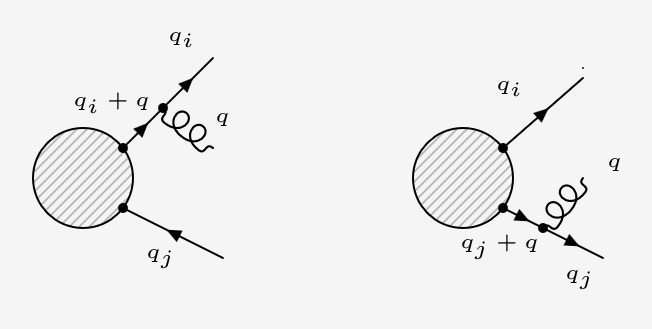
\includegraphics[width=0.85\textwidth]{images/QQ/qqg-diagrams.png}
\end{figure}
First we are going to consider a daughter quark from the splitting of a parent quark into a
quark and a gluon with an arbitrary spectator like an anti-quark, see the left picture above. where $ q_j+q $ is the momentum of the quark before splitting, $q$ the momentum of the gluon and $q_j$ of daughter quark respectively. The momentum of the spectator is $ q_j $. The distinction between daughter and parent vanishes, when the gluon becomes soft,  and a
singularity develops. The other possibility to get a singularity is surely if the gluon will be collinear to quark. The splitting functions are flavour independent since the strong interaction is flavour independent. Furthermore,
leading order splitting cannot change the flavour of a quark, thus we can write for the splitting functions In leading order QCD:
\begin{equation}
P_{{\bar{q_i}}{\bar{q_j}}}=P_{{q_i}{q_j}}=P_{{q}{q}} \delta_{ij}
\end{equation}
For this aim we have to take any diagram to the account which can have the same splitting. Since there is no distinction between quark and anti-quark, one can imagine exact the same splitting variation for anti-quark with a quark as a spectator, see the right picture above.


\pagebreak
\section{Matrix element of a quark with a gluon radiation $ |M_1|^2 $}

\begin{figure}[h!]
\centering
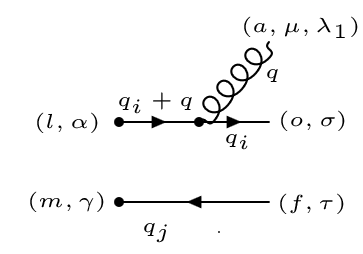
\includegraphics[scale=0.7]{images/QQ/qgqbarM.png}
\end{figure}
If one simply calculates the amplitude of this diagram, one gets:
\begin{equation}
M_1 = [{\bar{u}}_{\sigma}(q_i) (-ig_s \gamma^{\mu}\times {[T^a]_o}^l)  \frac{i(\not{q_i} + \not{q})}{(q_i + q)^2} {\varepsilon^{\lambda_1}}_{\mu} (q)]\: [{v}_{\tau}(q_j)]
\end{equation}
For the quadratic matrix element we need the dagger of $ M_1 $ as well.
\begin{figure}[h!]
\centering
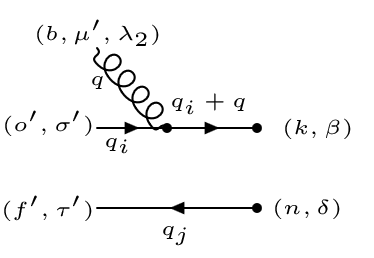
\includegraphics[scale=0.7]{images/QQ/qgqbarMDega.png}
\end{figure}

\begin{equation}
{M_1}^{\dagger} = [\frac{-i(\not{q_i} + \not{q})}{(q_i + q)^2} \:  (ig_s \gamma^{{\mu}^{\prime}}\times {[T^b]_{o\:^{\prime}}}^k) \: u_{{\sigma}^{\prime}}(q_i) \: {\varepsilon^{\lambda_2}}_{{\mu}^{\prime}} (q)][{\bar{v}}_{{\tau}^{\prime}}(q_j)]
\end{equation}
\pagebreak
\begin{figure}[h!]
\centering
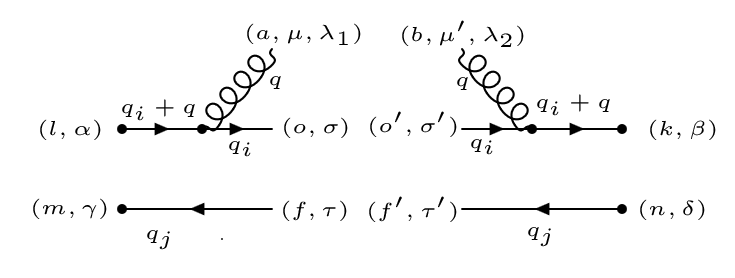
\includegraphics[width=0.85\textwidth]{images/QQ/qgqbarMSquer.png}
\end{figure}
After multiplying $ {M_1}^{\dagger} $ and $ {M_1} $ we get the desired result.
\begin{equation}
\begin{split}
|M_1|^2=M_1\:{\color[RGB]{255,0,0} {M_1}^{\dagger}} = [{\bar{u}}_{\sigma}(q_i)\: (-ig_s \gamma^{\mu}\times {[T^a]_o}^l) \: \frac{i(\not{q_i} + \not{q})}{(q_i + q)^2}\:\: {\varepsilon^{\lambda_1}}_{\mu} (q)] [{v}_{\tau}(q_j)]\: \\
\quad\quad\quad\quad\quad\quad\quad\quad\:\:{\color[RGB]{255,0,0}[\frac{-i(\not{q_i} + \not{q})}{(q_i + q)^2} \:  (ig_s \gamma^{{\mu}^{\prime}}\times {[T^b]_{o\:^{\prime}}}^k) \: u_{{\sigma}^{\prime}}(q_i) \: {{\varepsilon^{\lambda_2}}_{{\mu}^{\prime}}}^* (q)][{\bar{v}}_{{\tau}^{\prime}}(q_j)]}
\end{split}
\end{equation}
Now it's time to connect those terms which are related to each other.

\begin{equation}
\begin{split}
|M_1|^2=[\frac{-i(\not{q_i} + \not{q})}{(q_i + q)^2} \:
 \:  (ig_s \gamma^{{\mu}^{\prime}}\times {[T^b]_{o\:^{\prime}}}^k) \: {\bar{u}}_{\sigma}(q_i)\:u_{{\sigma}^{\prime}}(q_i) \: {{\varepsilon^{\lambda_2}}_{{\mu}^{\prime}}^* (q) {\varepsilon^{\lambda_1}}_{\mu} (q)} \\
\times (-ig_s \gamma^{\mu}\times {[T^a]_o}^l) \: \frac{i(\not{q_i} + \not{q})}{(q_i + q)^2} ]
[{\bar{v}}_{{\tau}^{\prime}}(q_j) {v}_{\tau}(q_j)]
\end{split}
\end{equation}

Sum over the lorenz index $({\sigma},{\sigma}^{\prime})$ and $({\tau},{\tau}^{\prime})$ and spin addition relation leads to:
 
\begin{equation}
\begin{split}
\displaystyle\sum\limits_{{\sigma},{\sigma}^{\prime}} {\bar{u}}_{\sigma}(q_i)\:u_{{\sigma}^{\prime}}(q_i) = \not{q_i} \delta^{{o}{o}^{\prime}},\\
\displaystyle\sum\limits_{{\tau},{\tau}^{\prime}} {\bar{v}}_{\tau}(q_j)\:v_{{\tau}^{\prime}}(q_j) = \not{q_j} \delta^{{f}{f}^{\prime}}
\end{split}
\end{equation}
Sum over polarization index $({\lambda_{1}},{\lambda}_{2})$ :
\begin{equation}
\begin{split}
 \displaystyle\sum\limits_{{\mu},{\mu}^{\prime}} {{\varepsilon^{\lambda_2}}_{{\mu}^{\prime}}^* (q) {\varepsilon^{\lambda_1}}_{\mu} (q)} = -g_{{\mu}{\mu}^{\prime}} \delta^{{a}{b}}
\end{split}
\end{equation}
The matrix element will be simplified with: 
\begin{equation}
\begin{split}
|M_1|^2=\frac{-g_s^2  {[T^a]_{o}}^k \: {[T^a]_o}^l }{(q_i + q)^2 (q_i + q)^2}
[(\not{q_i} + \not{q}) \:
 \:  \gamma^{{\mu}^{\prime}} \: \not{q_i} \: g_{{{\mu}^{\prime}}{\mu}} 
\gamma^{\mu} \: (\not{q_i} + q)]
[\not{q_j}]
\end{split}
\end{equation}

When we contract all related indices we will be actually able to make a statements about the last result.
\begin{equation}
\begin{split}
|M_1|^2=\frac{-g_s^2  {[T^a]_{o}}^k \: {[T^a]_o}^l }{(q_i + q)^2 (q_i + q)^2}
[(\not{q_i} + \not{q}) \:
 \:  \gamma^{{\mu}^{\prime}} \: \not{q_i} \: 
\gamma_{{\mu}^{\prime}} \: (\not{q_i} + q)]
[\not{q_j}]
\end{split}
\end{equation}

In other words we expect the tree level diagram from LO and a number:\\
\begin{figure}[h!]
\centering
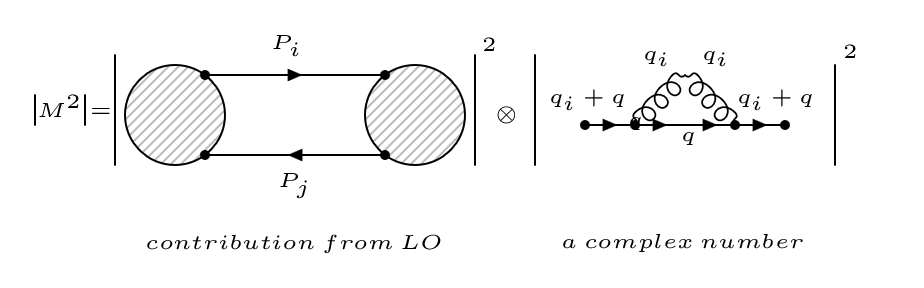
\includegraphics[width=0.85\textwidth]{images/QQ/expectationqg-qbar.png}
\end{figure}
Which graphically means:\\
\begin{equation}
\begin{split}
|M_1|^2=\frac{-g_s^2  {[T^a]_{o}}^k \: {[T^a]_o}^l }{(q_i + q)^2 (q_i + q)^2}
[\not{P_i}]
[\not{P_j}]\:\otimes \: {\color[RGB]{255,0,0} (a\: complex\: number)}
\end{split}
\end{equation}  
Let's calculate the contribution and compare the final result with this expectation:
\begin{equation}
\begin{split}
N=&: \gamma^{{\mu}^{\prime}} \not{q_i} \: \gamma_{{\mu}^{\prime}} = {q_{i\sigma}} \: \gamma^{{\mu}^{\prime}} \gamma^{\sigma} \:\: \gamma_{{\mu}^{\prime}}\\
=& \: {q_{i\sigma}} \: (\lbrace{\gamma^{{\mu}^{\prime}}}, {\gamma^{\sigma}}\rbrace \: - {\gamma^{\sigma}}{\gamma^{{\mu}^{\prime}}})\gamma_{{\mu}^{\prime}}\\
=& \:{q_{i\sigma}} \: 2g^{{{\mu}^{\prime}}{\sigma}} \: \gamma_{{\mu}^{\prime}} \: - \:d\:{\gamma^{\sigma}}\\
=& \:(2-d) \not{q_i}
\end{split}
\end{equation}
Simplification of the bracket:
\begin{equation}
\begin{split}
|M_1|^2=-(2-d)\:\frac{g_s^2  {[T^a]_{o}}^k \: {[T^a]_o}^l }{(q_i + q)^2 (q_i + q)^2}
[(\not{q_i} + \not{q}) \:
 \:\not{q_i} \: 
 \: (\not{q_i} + q)]
[\not{q_j}]
\end{split}
\end{equation}

\begin{equation}
\begin{split}
|M_1|^2=-(2-d)\:\frac{g_s^2  {[T^a]_{o}}^k \: {[T^a]_o}^l }{(q_i + q)^2 (q_i + q)^2}
[\not{q_i} \not{q_i} \not{q_i} \: + \: \not{q_i} \not{q_i} \not{q} \: + \: \not{q} \not{q_i} \not{q_i} \:+\: \not{q} \not{q_i} \not{q}]
[\not{q_j}]
\end{split}
\end{equation}

Momenta are on-shell, so:
\begin{equation}
\begin{split}
\not{q_i}\: \not{q_i} &= {q_i}^2= {m_i}^2\\
\not{q} \: \not{q} &= {q}^2= {m}^2\\
\not{q_j}\not{q_j} &= {q_j}^2= {m_j}^2
\end{split}
\end{equation}

we can first neglect the mass of patrons:

\begin{equation}
\begin{split}
|M_1|^2=-(2-d)\:\frac{g_s^2  {[T^a]_{o}}^k \: {[T^a]_o}^l }{(2q_i q)(2q_i q)}
[\not{q} \not{q_i} \not{q}]
[\not{q_j}]
\end{split}
\end{equation}
Here we need to make the terms in the brackets simpler and:
\begin{equation}
\begin{split}
L=& \not{q} \not{q_i} \not{q} =\not{q}[{q_{i\sigma}} q_{\mu} \: (\lbrace{\gamma^{\mu}}, {\gamma^{\sigma}}\rbrace - {\gamma^{\sigma}}{\gamma^{\mu}})]\\ 
=& \not{q}[2{q_{i}}^{\mu} q_{\mu} - {q_{i\sigma}}q_{\mu}{\gamma^{\mu}}{\gamma^{\sigma}}\\
=& \not{q} (2q_i q)-q_{\mu}{q_{i\sigma}}q_{\mu}[{\gamma^{\mu}}{\gamma^{\mu}}{\gamma^{\sigma}}]\\
=& \not{q} (2q_i q)-q_{\mu}{q_{i\sigma}}q_{\mu}[\frac{{\gamma^{\mu}}{\gamma^{\mu}}}{2} +\frac{{\gamma^{\mu}}{\gamma^{\mu}}}{2}]{\gamma^{\sigma}}\\
=& \not{q} (2q_i q)-q_{\mu}{q_{i\sigma}}q_{\mu}[g^{{\mu}{\mu}}]{\gamma^{\sigma}}\\
=& \not{q} (2q_i q)-q_{\mu}{q_{i\sigma}}q^{\mu}{\gamma^{\sigma}}
=\not{q} (2q_i q)-q^2 \not{q_i}\\
=& \not{q} (2q_i q)
\end{split}
\end{equation}
After inserting the last result of $ L $ and simplify the term $ (2q_i q) $ from the denominator and nominator, we get:
\begin{equation}
\begin{split}
|M_1|^2=-(2-d)\:\frac{g_s^2  {[T^a]_{o}}^k \: {[T^a]_o}^l }{2y(1-2z+2z^2)(p_i \cdot p_j)}
[\not{q}]
[\not{q_j}]
\end{split}
\end{equation}
Now we are going to use the parametrisation from equation (1) to reduce the 3-member matrix element to 2-member and take out the singularity term from the amplitude.
\begin{equation}
\begin{split}
|M_1|^2=(d-2)\:\frac{g_s^2  {[T^a]_{o}}^k \: {[T^a]_o}^l }{2y(1-2z+2z^2)(p_i \cdot p_j)}
[(1-z) \not{p_i}+zy \not{p_j} - \sqrt{zy(1-z)} \not{{m}_{\bot}}]
[(1-y) \not{p_j}]
\end{split}
\end{equation}
Multiplying the both sides 
\begin{equation}
\begin{split}
|M_1|^2=(d-2)\:\frac{g_s^2  {[T^a]_{o}}^k \: {[T^a]_o}^l }{2y(1-2z+2z^2)(p_i \cdot p_j)}
[(1-z)(1-y) \not{p_i}\not{p_j} \\
+zy(1-y) \not{p_j}\not{p_j} + (1-y)\sqrt{zy(1-z)} \not{{m}_{\bot}}\not{p_j}]
\end{split}
\end{equation}
Under consideration of the fact that $ p_i $ and $ p_j $ are the on-shell momenta of the emitter and spectator partons, we can ignore the terms with $ \not{p_i} \not{p_i} $ and $ \not{p_j} \not{p_j} $.
The $ {p_i} \cdot  {m}_{\bot} $ and $ {p_j} \cdot  {m}_{\bot} $ are always $ 0 $ because the $ p_i $ and $ p_j $ are lightlike, i.e. zero transverse component. So those terms can be neglected.


\begin{equation}
\begin{split}
|M_1|^2=\frac{g_s^2  {[T^a]_{o}}^k \: {[T^a]_o}^l }{(p_i \cdot p_j)}
[\not{p_i}][\not{p_j}]\otimes\frac{(d-2)(1-z)(1-y)}{2y(1-2z+2z^2)}
\end{split}
\end{equation}

As discussed, we get a contribution from the LO a complex number. As you can see, the number is just for $ y \rightarrow 0 $ singular and not for $ z \rightarrow 1 $.

\newpage

\section{Matrix element of an anti-quark with a gluon radiation $ |M_2|^2 $}

%\begin{figure}[h!]
%\centering
%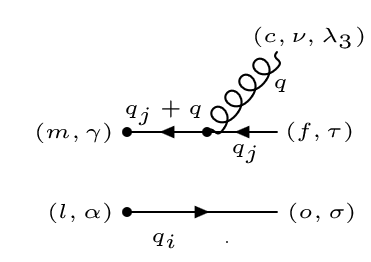
\includegraphics[scale=0.7]{images/QQ/qbargqM.png}
%\end{figure}
%
%\begin{equation}
%M_2 = [\frac{i(\not{q_j} + \not{q})}{(q_j + q)^2} (-ig_s \gamma^{\nu}\times {[T^c]_f}^m) \:{v}_{\tau}(q_j)\: {\varepsilon^{\lambda_3}}_{\nu} (q)]\: [{u}_{\sigma}(q_i)]
%\end{equation}
%\begin{figure}[h!]
%\centering
%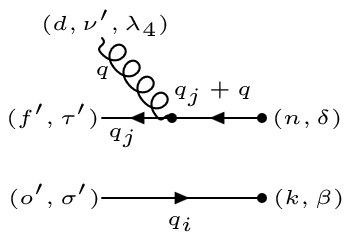
\includegraphics[scale=0.7]{images/QQ/qbargqMDega.png}
%\end{figure}
%\begin{equation}
%M_2^{\dagger} = [\bar{v}_{{\tau}^{\prime}}(q_j) \: (ig_s \gamma^{{\nu}^{\prime}}\times {[T^d]_{f^{\prime}}}^n) \: \frac{-i(\not{q_j} + \not{q})}{(q_j + q)^2} \: {\varepsilon^{\lambda_4}}_{{\nu}^{\prime}} (q)]\: [\bar{u}_{{\sigma}^{\prime}}(q_i)]
%\end{equation}
the same procedure is used to obtain the matrix element for an anti-quark with a single gluon emission.
\begin{figure}[h!]
\centering
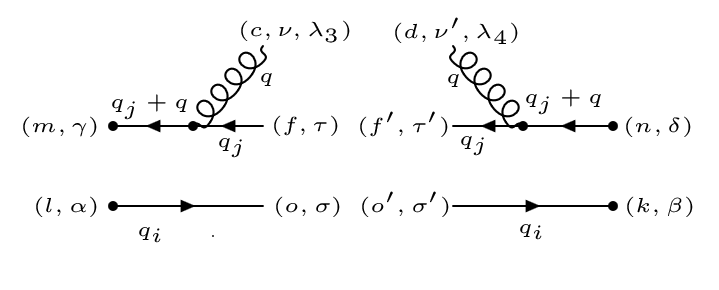
\includegraphics[width=0.85\textwidth]{images/QQ/qbargqMSquer.png}
\end{figure}

\begin{equation}
\begin{split}
|M_2|^2=M_2\:{\color[RGB]{255,0,0} {M_2}^{\dagger}} = [\frac{i(\not{q_j} + \not{q})}{(q_j + q)^2} (-ig_s \gamma^{\nu}\times {[T^c]_f}^m) \:{v}_{\tau}(q_j)\: {\varepsilon^{\lambda_3}}_{\nu} (q)]\: [{u}_{\sigma}(q_i)]\: \\
\quad\quad\quad\quad\quad\quad\quad\quad\:\:{\color[RGB]{255,0,0}[\bar{v}_{{\tau}^{\prime}}(q_j) \: (ig_s \gamma^{{\nu}^{\prime}}\times {[T^d]_{f^{\prime}}}^n) \: \frac{-i(\not{q_j} + \not{q})}{(q_j + q)^2} \: {\varepsilon^{\lambda_4}}_{{\nu}^{\prime}} (q)]\: [\bar{u}_{{\sigma}^{\prime}}(q_i)]}
\end{split}
\end{equation}


\begin{equation}
\begin{split}
|M_2|^2 =\frac{g_s^2 \: {[T^c]_f}^m \: {[T^d]_{f^{\prime}}}^n }{(q_j + q)^2 (q_j + q)^2} [(\not{q_j} + \not{q}) \gamma^{\nu}  \:{v}_{\tau}(q_j)\bar{v}_{{\tau}^{\prime}}(q_j)\: {\varepsilon^{\lambda_3}}_{\nu} (q){\varepsilon^{\lambda_4}}_{{\nu}^{\prime}}  (q) \gamma^{{\nu}^{\prime}}(\not{q_j} + \not{q})]\: \\
[{u}_{\sigma}(q_i) ]
\: [\bar{u}_{{\sigma}^{\prime}}(q_i)]
\end{split}
\end{equation}

and after sum over the lorenz and polarization indexes like $({\sigma},{\sigma}^{\prime})$, $({\tau},{\tau}^{\prime})$ and $({\lambda_{3}},{\lambda}_{4})$ as well and using the spin addition relation:
 
%\begin{equation}
%\begin{split}
%\displaystyle\sum\limits_{{\sigma},{\sigma}^{\prime}} {\bar{u}}_{\sigma}(q_i)\:u_{{\sigma}^{\prime}}(q_i) = \not{q_i} \delta^{{o}{o}^{\prime}},\\
%\displaystyle\sum\limits_{{\tau},{\tau}^{\prime}} {\bar{v}}_{\tau}(q_j)\:v_{{\tau}^{\prime}}(q_j) = \not{q_j} \delta^{{f}{f}^{\prime}}
%\end{split}
%\end{equation}
%
%\begin{equation}
%\begin{split}
% \displaystyle\sum\limits_{{\nu},{\nu}^{\prime}} {{\varepsilon^{\lambda_4}}_{{\nu}^{\prime}}^* (q) {\varepsilon^{\lambda_3}}_{\nu} (q)} = -g_{{\nu}{\nu}^{\prime}} \delta^{{c}{d}}
%\end{split}
%\end{equation}

\begin{equation}
\begin{split}
|M_2|^2 =\frac{g_s^2 \: {[T^c]_f}^m \: {[T^c]_{f}}^n }{(q_j + q)^2 (q_j + q)^2} [(\not{q_j} + \not{q}) \gamma^{\nu}  \:\not{q_j}\: (-g_{{\nu}{{\nu}^{\prime}}}) \gamma^{{\nu}^{\prime}}(\not{q_j} + \not{q})]\: 
[\not{q_i} ]
\end{split}
\end{equation}

Analogous to the last calculation from the previous section:

\begin{equation}
\begin{split}
|M_2|^2 =(d-2) \frac{g_s^2 \: {[T^c]_f}^m \: {[T^c]_{f}}^n }{(2qq_j)} [\not{q}]\: 
[\not{q_i} ]
\end{split}
\end{equation}
finally, we achieve:
\begin{equation}
\begin{split}
|M_2|^2=\frac{g_s^2 \: {[T^c]_f}^m \: {[T^c]_{f}}^n }{(p_i \cdot p_j)}
[\not{p_i}][\not{p_j}]\otimes \frac{-(d-2)yz^2}{2(1-z)(1-y)}
\end{split}
\end{equation}
Interestingly, here is a term with $y$ concerning the gluon radiation from an anti-quark. This means that this result cannot contribute to the collinear limit for soft gluon $ y \rightarrow 0 $.
\newpage

\section{Interference contribution}
So far most of the work is done and we just have to put the results of $M_1$ and ${M_2}^{\dagger}$ next to each other, as we can see in the diagram. So we still get the interference contribution. 
\begin{figure}[h!]
\centering
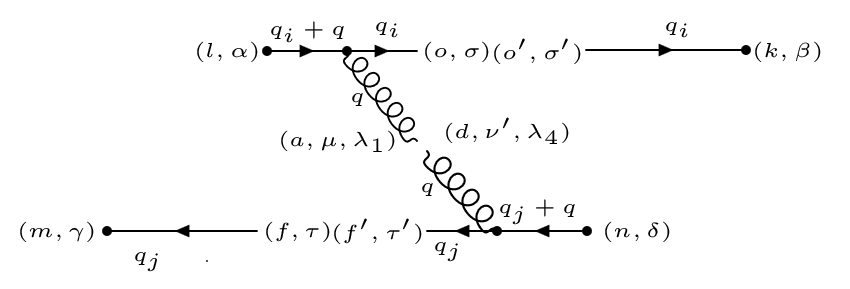
\includegraphics[width=0.85\textwidth]{images/QQ/M1M2Degaqqg.png}
\end{figure}
Using the results from the previous section and we received:
\begin{equation}
\begin{split}
M_1\:{\color[RGB]{255,0,0} {M_2}^{\dagger}} = [{\bar{u}}_{\sigma}(q_i)\: (-ig_s \gamma^{\mu}\times {[T^a]_o}^l) \: \frac{i(\not{q_i} + \not{q})}{(q_i + q)^2}\:\: {\varepsilon^{\lambda_1}}_{\mu} (q)] [{v}_{\tau}(q_j)]\: \\
\quad\quad\quad\quad\quad\quad\quad\quad\:\:{\color[RGB]{255,0,0}[\bar{v}_{{\tau}^{\prime}}(q_j) \: (ig_s \gamma^{{\nu}^{\prime}}\times {[T^d]_{f^{\prime}}}^n) \: \frac{-i(\not{q_j} + \not{q})}{(q_j + q)^2} \: {\varepsilon^{\lambda_4}}_{{\nu}^{\prime}} (q)]\: [{u}_{{\sigma}^{\prime}}(q_i)]}
\end{split}
\end{equation}

%Kommentar

\begin{equation}
\begin{split}
M_1\: {M_2}^{\dagger} = \frac{g_s^2 {[T^a]_o}^l \:{[T^d]_{f^{\prime}}}^n }{(2q_i q)(2q_j q)} [\not{q_i}\: \gamma^{\mu} \: (\not{q_i} + \not{q})\: ]{\varepsilon^{\lambda_1}}_{\mu} (q) \: {\varepsilon^{\lambda_4}}_{{\nu}^{\prime}} (q) \\
\:[\not{q_j} \:\gamma^{{\nu}^{\prime}} \: (\not{q_j} + \not{q})]\:
\end{split}
\end{equation}

\begin{equation}
\begin{split}
M_1\: {M_2}^{\dagger} = \frac{g_s^2 {[T^a]_o}^l \:{[T^a]_{f^{\prime}}}^n }{(2q_i q)(2q_j q)} [\not{q_i}\: \gamma^{\mu} \: (\not{q_i} + \not{q})\: ] -g_{{\mu}{{\nu}^{\prime}}} \\
\:[\not{q_j} \:\gamma^{{\nu}^{\prime}} \: (\not{q_j} + \not{q})]\:
\end{split}
\end{equation}



\begin{equation}
\begin{split}
M_1\: {M_2}^{\dagger} = \frac{-g_s^2 {[T^a]_o}^l \:{[T^a]_{f^{\prime}}}^n }{(2q_i q)(2q_j q)} [\not{q_i}\: \gamma^{\mu} \: (\not{q_i} + \not{q})\: ]
\:[\not{q_j} \:\gamma_{\mu} \: (\not{q_j} + \not{q})]\:
\end{split}
\end{equation}

%Kommentar 

Expectation:
\begin{figure}[h!]
\centering
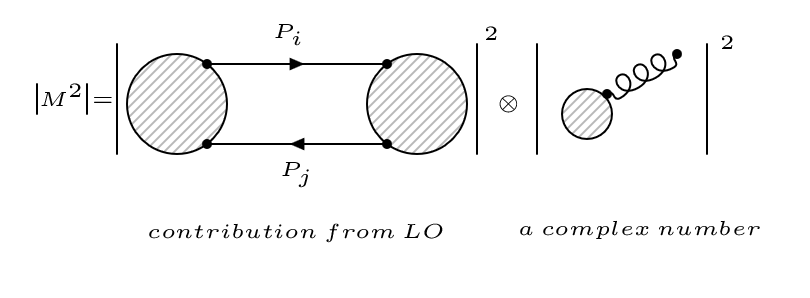
\includegraphics[width=0.85\textwidth]{images/QQ/expectationM1M2dagger.png}
\end{figure}

%Kommentar

\begin{equation}
\begin{split}
M_1\: {M_2}^{\dagger} = \frac{-g_s^2 {[T^a]_o}^l \:{[T^a]_{f^{\prime}}}^n }{(2q_i q)(2q_j q)} [(\not{q_i} + \not{q})\: \gamma^{\mu} \:  \not{q_i}\:]
\:[(\not{q_j} + \not{q}) \:\gamma_{\mu} \:\not{q_j} ]\:
\end{split}
\end{equation}

%Kommentra

\begin{align}
\begin{split}
&M_1\: {M_2}^{\dagger} = \frac{-g_s^2 {[T^a]_o}^l \:{[T^a]_{f^{\prime}}}^n }{(2q_i q)(2q_j q)} [-(\not{q_i} + \not{q})\:\not{q_i}\: \gamma^{\mu} \:+2(\not{q_i} + \not{q})\:{q_{i}}^{\mu}]\:\:\:\:\:\:\:\:\:\:\:\:\:\:\:\:\:\:\:\:\:\:\:\:\:\:\:\:\:\:\:\:\:\:\:\:\:\:\:\:\:\:\\
&\:[-(\not{q_j} + \not{q}) \not{q_j} \:\gamma_{\mu} \: + 2(\not{q_j} + \not{q}) {q_{j{\mu}}}]\: \\
\Rightarrow
&M_1\: {M_2}^{\dagger} = \frac{-g_s^2 {[T^a]_o}^l \:{[T^a]_{f^{\prime}}}^n }{(2q_i q)(2q_j q)} 
[(\not{q_i} + \not{q})\:\not{q_i}\: \gamma^{\mu}] \:[(\not{q_j} + \not{q}) \not{q_j} \gamma_{\mu}] \\
&-2[(\not{q_i} + \not{q})\:\not{q_i}\: \gamma^{\mu}]\:[ (\not{q_j} + \not{q}) {q_{j{\mu}}}]
\:-2[(\not{q_i} + \not{q})\:{q_{i}}^{\mu}][(\not{q_j} + \not{q}) \not{q_j} \:\gamma_{\mu}]\\
&+4[(\not{q_i} + \not{q})\:{q_{i}}^{\mu}][(\not{q_j} + \not{q}) {q_{j{\mu}}}]
\end{split}
\end{align}
The middle terms disappear due to the influence of the gamma matrices if the sequence of the matrices is reversed, so that the two terms become the same, because $ AB = -BA $:

%Kommentar

\begin{equation}
\begin{split}
&M_1\: {M_2}^{\dagger} = \frac{-g_s^2 {[T^a]_o}^l \:{[T^a]_{f^{\prime}}}^n }{(2q_i q)(2q_j q)} 
[(\not{q_i} + \not{q})\:\not{q_i}\: \gamma^{\mu}] \:[(\not{q_j} + \not{q}) \not{q_j} \gamma_{\mu}] \\
&-2[(\not{q_i} + \not{q})\:\not{q_i}\:\not{q_{j}} ]\:[ \not{q_j} + \not{q} ]
\:-2[\not{q_i} + \not{q}\:][(\not{q_j} + \not{q}) \not{q_j} \:\not{q_i}]\\
&+4[(\not{q_i} + \not{q})\:{q_{i}}^{\mu}][(\not{q_j} + \not{q}) {q_{j{\mu}}}]
\end{split}
\end{equation}

%Kommentar

\begin{align}
\begin{split}
&M_1\: {M_2}^{\dagger} = \frac{-g_s^2 {[T^a]_o}^l \:{[T^a]_{f^{\prime}}}^n }{(2q_i q)(2q_j q)} 
[(\not{q_i} + \not{q})\:\not{q_i}\: \gamma^{\mu}] \:[(\not{q_j} + \not{q}) \not{q_j} \gamma_{\mu}]\:\:\:\:\:\:\:\:\:\:\:\:\:\:\:\:\:\:\:\:\:\: \\
&+4[(\not{q_i} + \not{q})\:{q_{i}}^{\mu}][(\not{q_j} + \not{q}) {q_{j{\mu}}}]
\end{split}
\end{align}
Now we use the old parametrization to collect the singularities.
%\begin{equation}
%\begin{split}
%&M_1\: {M_2}^{\dagger} = \frac{-g_s^2 \:\:{[T^a]_o}^l \:{[T^a]_{f^{\prime}}}^n }{4(1-z)(1-y)y(1-2z+2z^2)(p_i \cdot p_j)(p_i \cdot p_j)} \\
%&[y(1-2z+2z^2)\not{p_i}\:\not{p_j}\: \gamma^{\mu}] \:[(1-z)(1-y)\not{p_i} \not{p_j} \gamma_{\mu}] \\
%&+4({q_{i}}^{\mu} \cdot {q_{j{\mu}}})[(\not{q_i} + \not{q})][(\not{q_j} + \not{q})]
%\end{split}
%\end{equation}

\begin{align}
\begin{split}
&M_1\: {M_2}^{\dagger} = \frac{-g_s^2 \:\:{[T^a]_o}^l \:{[T^a]_{f^{\prime}}}^n }{4(1-z)(1-y)y(1-2z+2z^2)(p_i \cdot p_j)(p_i \cdot p_j)} \\
&[y(1-2z+2z^2)\not{p_i}\:\not{p_j}\: \gamma^{\mu}] \:[(1-z)(1-y)\not{p_i} \not{p_j} \gamma_{\mu}] \\
&+4(p_i \cdot p_j)[(\not{p_i} + y\not{p_j})][(1-z)\not{p_i} + (1+yz-y) \not{p_j} - \sqrt{zy(1-z)}\not{m}]
\end{split}
\end{align}
Here we can use the singular term in the denominator $ y(1-z) $ to drop the term with the same pre-factor and thus obtain:

\begin{align}
\begin{split}
&M_1\: {M_2}^{\dagger} = \frac{-g_s^2 \:\:{[T^a]_o}^l \:{[T^a]_{f^{\prime}}}^n }{y(1-2z+2z^2)(p_i \cdot p_j)} 
[\not{p_i}][\not{p_j}]\otimes\frac{z}{1-z}\:\:\:\:\:\:\:\:\:\:\:\:\:
\end{split}
\end{align}

\pagebreak

\section{Final result}
One could assume that for a complete result the contribution $ {M_1}^{\dagger} M_2 $ is still missing.
\begin{equation}
\lvert\:M\lvert^2\: = \lvert\:M_1\lvert^2\:+\lvert\:M_2\lvert^2\:+ M_1\: {M_2}^{\dagger} +{M_1}^{\dagger} M_2
\end{equation}
\begin{figure}[h!]
\centering
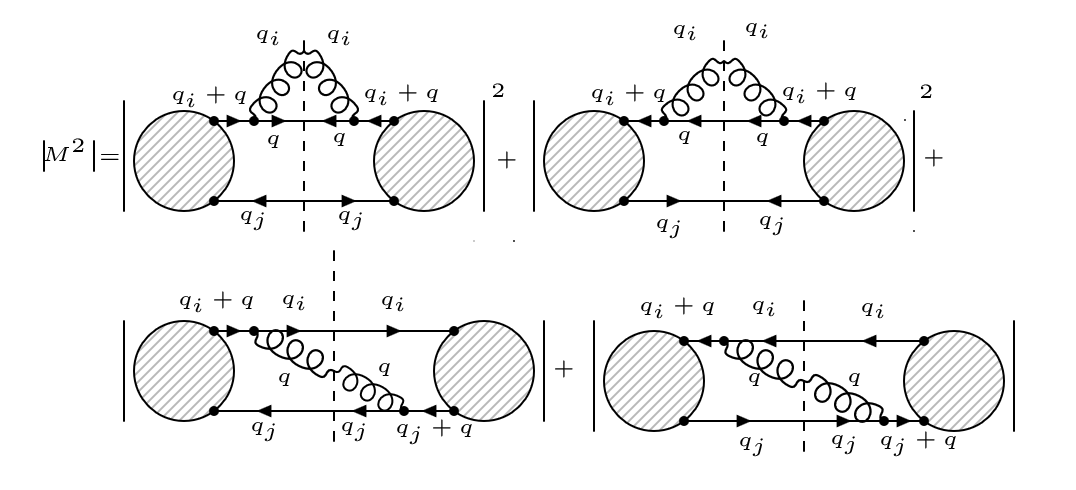
\includegraphics[width=0.85\textwidth]{images/QQ/qqgMSquer.png}
\end{figure}
It should be noted that it is completely sufficient to calculate $M_1\: {M_2}^{\dagger}$, because we know it from the quadratic amount of the complex numbers, we can calculate double of real part of $2RE(M_1\: {M_2}^{\dagger})$ instead of $ M_1\: {M_2}^{\dagger} +{M_1}^{\dagger} M_2 $ and that is exactly what is preferred here.
\begin{equation}
\lvert\:M\lvert^2\: = \lvert\:M_1\lvert^2\:+\lvert\:M_2\lvert^2\:+ {\color[RGB]{255,0,0} 2RE(M_1\: {M_2}^{\dagger})}
\end{equation}
\begin{figure}[h!]
\centering
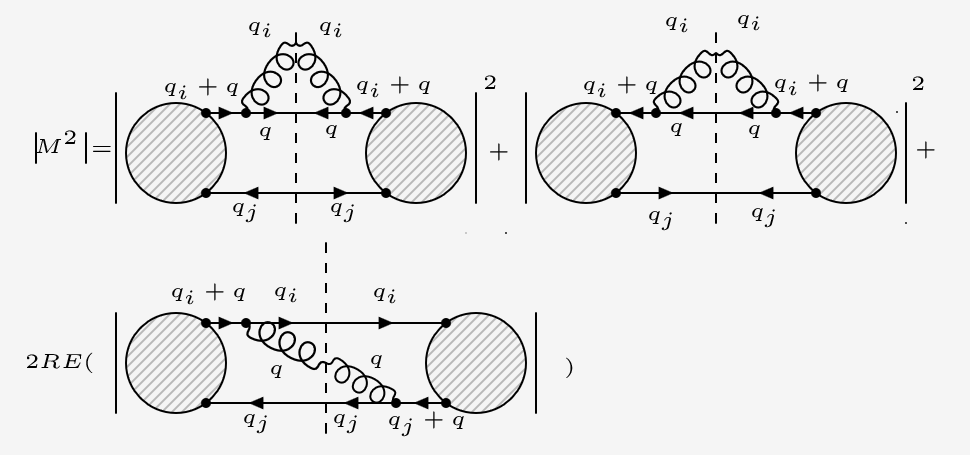
\includegraphics[width=0.85\textwidth]{images/QQ/REqqgMSquer.png}
\end{figure}
Let's just add up the results from the previous sections and get:
\begin{equation}
\begin{split}
&\lvert\:M\lvert^2\: = (d-2)(1-z)(1-y)\:\frac{g_s^2  {[T^a]_{o}}^k \: {[T^a]_o}^l }{2y(1-2z+2z^2)(p_i \cdot p_j)}
[\not{p_i}][\not{p_j}]\\
&-(d-2)yz^2\:\frac{g_s^2 \: {[T^c]_f}^m \: {[T^c]_{f}}^n }{2(1-z)(1-y)(p_i \cdot p_j)}
[\not{p_i}][\not{p_j}]\\
&+2RE((\frac{-2z}{z-1}) \frac{g_s^2 \:\:{[T^a]_o}^l \:{[T^a]_{f}}^n }{2y(1-2z+2z^2)(p_i \cdot p_j)} 
[\not{p_i}][\not{p_j}])
\end{split}
\end{equation}
Now we use the knowledge from the introduction about the calculation of the Colour factor. With Fritz equation:
\begin{equation}
{T^a}_{o\:k} \: {T^a}_{l\:o} = \frac{1}{2}(\delta_{oo}\delta_{lk}-\frac{1}{N}\delta_{ok}\delta_{lo})= \frac{1}{2}(N\delta_{lk}-\frac{1}{N}\delta_{lk})=C_F \delta_{lk}
\end{equation}
After summation over the final colour states and averaging over initial colour states we get:

\begin{equation}
{T^a}_{o\:k} \: {T^a}_{l\:o}=C_F \delta_{lk}=\frac{1}{N} \displaystyle\sum\limits_{l=1}^ N \delta_{lk}C_F=C_F
\end{equation}
The same calculation for $ {T^c}_{m\:f} \: {T^c}_{f\:n} $ and $ {T^a}_{o\:l} \: {T^a}_{f\:n} $ turns $ C_F $ out as the colour factor.
Now we are going to compute the splitting function in the case of the colinearity, wich means, if:
\begin{equation}
y \longrightarrow 0
\end{equation}

%\begin{equation}
%\begin{split}
%&\lvert\:M\lvert^2\: = (d-2)(1-z)(1-y)\:\frac{g_s^2 C_F}{2y(1-2z+2z^2)(p_i \cdot p_j)}
%[\not{p_i}][\not{p_j}]\\
%&-(d-2)yz^2\:\frac{g_s^2 \: C_F }{2(1-z)(1-y)(p_i \cdot p_j)}
%[\not{p_i}][\not{p_j}]\\
%&+2RE((\frac{-2z}{z-1}) \frac{g_s^2 C_F}{2y(1-2z+2z^2)(p_i \cdot p_j)} 
%[\not{p_i}][\not{p_j}]
%\end{split}
%\end{equation}

\begin{equation}
\lvert\:M\lvert^2\: = \frac{g_s^2 C_F}{2y(1-2z+2z^2)(p_i \cdot p_j)}[\not{p_i}][\not{p_j}] \otimes((d-2)(1-z)-\frac{4z}{z-1})\:
\end{equation}
\\
for $ d=4-2\epsilon $

%\begin{equation}
%\begin{split}
%\lvert\:M\lvert^2\: = C_F((4-2\epsilon-2)(1-z)+\frac{4z}{1-z})\:\frac{g_s^2}{2y(1-2z+2z^2)(p_i \cdot p_j)}[\not{p_i}][\not{p_j}]\\
%=C_F(\frac{2(1-\epsilon)(1-z)^2+4z}{1-z})\:\frac{g_s^2}{2y(1-2z+2z^2)(p_i \cdot p_j)}[\not{p_i}][\not{p_j}]\\
%C_F(\frac{2-4z+2z^2-\epsilon(1-z)^2+4z}{1-z})\:\frac{g_s^2}{2y(1-2z+2z^2)(p_i \cdot p_j)}[\not{p_i}][\not{p_j}]\\
%=C_F(\frac{(1+z^2)}{1-z}-\epsilon(1-z))\:\frac{g_s^2}{y(1-2z+2z^2)(p_i \cdot p_j)}[\not{p_i}][\not{p_j}]\\
%=\langle\:\hat{P_{qq}}\rangle\:\frac{g_s^2}{q_i \cdot q}[\not{p_i}][\not{p_j}]\\
%\end{split}
%\end{equation}

\begin{equation}
\begin{split}
\lvert\:M\lvert^2\: &=\frac{g_s^2}{y(1-2z+2z^2)(p_i \cdot p_j)}[\not{p_i}][\not{p_j}]\otimes C_F(\frac{(1+z^2)}{1-z}-\epsilon(1-z))\\
&=\frac{g_s^2}{q_i \cdot q}[\not{p_i}][\not{p_j}]\otimes \langle\:\hat{P_{qq}}\rangle\:\\
\end{split}
\end{equation}

With Alterali-Parisi splitting function $ \langle\:\hat{P_{qq}}\rangle\: $ in the collinear limes, which was mentioned in the previous chapter. This is exactly the confirmation of our calculation that our calculation was actually performed correctly, otherwise we would not have received the same splitting function for soft gluons.
\newpage

\section{Double-check the results with the new kinematic}
One could do exactly the same calculation for the new kinematics to see if you get the same result in the collinear limit. From the next chapter we will explicitly work with the new parametrisation, because we found that the old kinematics only work in NLO and one-single emission. 
\subsection*{$ |M_1|^2 $}

\begin{equation}
\begin{split}
|M_1|^2=(d-2)\:\frac{g_s^2  C_F }{(2k_1\cdot q_i)}
[\not{k_1} ][\not{q_k}]
\end{split}
\end{equation}

\begin{equation}
\begin{split}
&|M_1|^2=(d-2)\:\frac{g_s^2 \: C_F }{2y\: p_i \cdot Q}
[(\alpha_1 -y\beta_1(\frac{Q^2}{2p_i \cdot Q})) \not{p_i} + y\beta_1\not{Q} + \sqrt{y\alpha_1\beta_1}\not{n}_{\bot,1} ]\\
&[A_1\not{p_i} + A_2\not{Q} + \sqrt{1-y}\not{p_k}]
\end{split}
\end{equation}

\begin{equation}
\begin{split}
&|M_1|^2=(d-2)\:\frac{g_s^2 \: C_F }{2y\: p_i \cdot Q}
[(A_2(\alpha_1 -y\beta_1(\frac{Q^2}{2p_i \cdot Q}))+ A_1y\beta_1) {p_i}\cdot Q\\
&+(\alpha_1 -y\beta_1(\frac{Q^2}{2p_i \cdot Q}))\sqrt{1-y}p_i\cdot p_k+A_2 y\beta_1 Q^2+ \sqrt{1-y}\sqrt{y\alpha_1\beta_1}{n}_{\bot,1}\cdot p_k ]\\
\end{split}
\end{equation}

For the collinearity $ y \rightarrow 0 $ we'll get:

\begin{equation}
\begin{split}
&|M_1|^2=(d-2)\:\frac{g_s^2 \: C_F }{2y\: p_i \cdot Q}
[(A_2(\alpha_1 -y\beta_1(\frac{Q^2}{2p_i \cdot Q}))+ A_1y\beta_1) \not{p_i} \not{Q}\\
&+(\alpha_1 -y\beta_1(\frac{Q^2}{2p_i \cdot Q}))\sqrt{1-y}\not{p_i} \not{p_k}+A_2 y\beta_1 Q^2+ \sqrt{1-y}\sqrt{y\alpha_1\beta_1}\not{n}_{\bot,1} \not{p_k} ]\\
\end{split}
\end{equation}

\begin{equation}
\begin{split}
&|M_1|^2=(d-2)(1-\beta_1)\sqrt{1-y}\:\frac{g_s^2 \: C_F }{2y\: p_i \cdot Q}
[\not{p_i} \not{p_k} ]\\
\end{split}
\end{equation}

\subsection*{$ |M_2|^2 $}

\begin{equation}
\begin{split}
|M_2|^2 =(d-2) \frac{g_s^2 \: C_F }{2k_1 \cdot q_k} [\not{k_1}]\: 
[\not{q_i} ]
\end{split}
\end{equation}

\begin{equation}
\begin{split}
&|M_2|^2 =(d-2) \frac{g_s^2 \: C_F}{2k_1 \cdot q_k} [(\alpha_1 -y\beta_1(\frac{Q^2}{2p_i \cdot Q})) \not{p_i} + y\beta_1\not{Q} + \sqrt{y\alpha_1\beta_1}\not{n}_{\bot,1}]\: \\
&[(\beta_1 -\alpha_1 y(\frac{Q^2}{2p_i \cdot Q}))\not{p_i} + y\alpha_1\not{Q} - \sqrt{y\alpha_1\beta_1}\not{n}_{\bot,l} ]
\end{split}
\end{equation}

Which means:
\begin{equation}
\begin{split}
&|M_2|^2 \sim(d-2) \frac{g_s^2 \: C_F}{2k_1 \cdot q_k} y[...]\\
&\:\:\:\:\:\:\:\:|M_2|^2\rightarrow 0 \:\:\:\:\:\:\:\text{for}\:\:\:\:\: y\rightarrow 0
\end{split}
\end{equation}

\subsection*{$ M_1\: {M_2}^{\dagger} $}


\begin{equation}
\begin{split}
&M_1\: {M_2}^{\dagger} = \frac{-g_s^2\: C_F }{4y(1-\beta_1) (1-y)\:(p_i \cdot p_k)(p_i \cdot Q)} \\
&4(\beta_1 \sqrt{1-y}{p_i}\cdot {{p_k}})[\beta_1 \sqrt{1-y}\not{p_i} \not{p_k}+ (1-\beta_1) \sqrt{1-y}\not{p_i}\not{p_k}]
\end{split}
\end{equation}

\begin{equation}
\begin{split}
&M_1\: {M_2}^{\dagger} = \frac{-g_s^2\: C_F }{y(1-\beta_1) \:(p_i \cdot p_k)(p_i \cdot Q)} \beta_1( {p_i}\cdot {{p_k}})[\beta_1 \not{p_i} \not{p_k}+ (1-\beta_1) \not{p_i}\not{p_k}]
\end{split}
\end{equation}

\begin{equation}
\begin{split}
&M_1\: {M_2}^{\dagger} = \frac{\beta_1}{(1-\beta_1)}\: \frac{-g_s^2\: C_F }{y \:(p_i \cdot Q)} [\not{p_i} \not{p_k}]
\end{split}
\end{equation}
\newpage
\newpage
\chapter{Gluon gluon gluon emission kernel}

\begin{figure}[ht!]
\centering
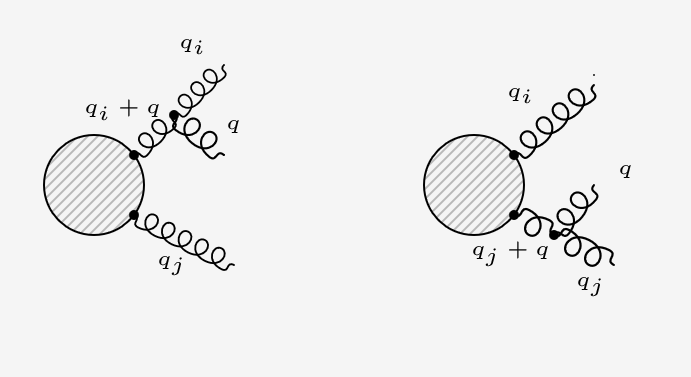
\includegraphics[width=0.85\textwidth]{images/GG/GGDiagrams.png}
\end{figure}
\pagebreak
\section{Gluon-Emitter Bubble}
\begin{figure}[ht!]
\centering
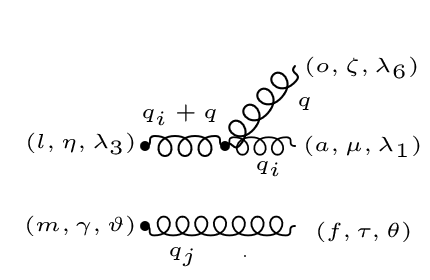
\includegraphics[scale=0.7]{images/GG/M1gg.png}
\end{figure}
\begin{equation}
\begin{split}
M_1=[\frac{-i}{(q +q_i)^2}(-g_s f^{\:a\:o\:l}(g^{{\mu}{\zeta}}(q -q_i)^{\eta}+g^{{\zeta}{\eta}}(-q-(q +q_i))^{\mu}+g^{{\eta}{\mu}}(q_i +q_i+q)^{\zeta})\\
{\varepsilon^{\lambda_1}}_{\mu} (q) {\varepsilon^{\lambda_6}}_{\zeta} (q)][{{\varepsilon^{\theta}}_{{\tau}^{\prime}}} (q_j)]
\end{split}
\end{equation}

\begin{equation}
\begin{split}
M_1=[\frac{-i}{(q_i +q)^2}(-g_s f^{\:a\:o\:l}(g^{{\mu}{\zeta}}(q-q_i)^{\eta}-g^{{\zeta}{\eta}}(2q +q_i)^{\mu}+g^{{\eta}{\mu}}(2q_i +q)^{\zeta})\\
{\varepsilon^{\lambda_1}}_{\mu} (q_i) {\varepsilon^{\lambda_6}}_{\zeta} (q)][{{\varepsilon^{\theta}}_{{\tau}^{\prime}}} (q_j)]
\end{split}
\end{equation}
\begin{figure}[ht!]
\centering
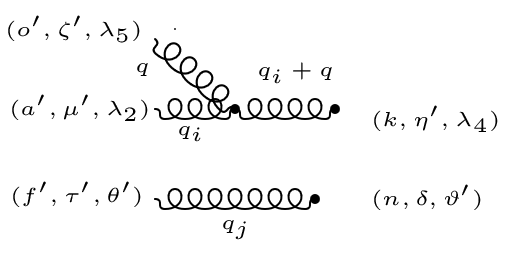
\includegraphics[scale=0.7]{images/GG/M1Daggergg.png}
\end{figure}
\begin{equation}
\begin{split}
{M_1}^{\dagger}=[\frac{i}{(q_i +q)^2}(-g_s f^{\:a^{\prime}\:k\: o^{\prime}}(-g^{{{\mu}^{\prime}}{{\eta}^{\prime}}}(2q_i+q)^{{\zeta}^{\prime}}+g^{{{\eta}^{\prime}}{{\zeta}^{\prime}}}(2q +q_i)^{{\mu}^{\prime}}+g^{{{\zeta}^{\prime}}{{\mu}^{\prime}}}(q_i-q)^{{\eta}^{\prime}})\\
{{\varepsilon^{\lambda_2}}_{{\mu}^{\prime}}}^* (q_i) {{\varepsilon^{\lambda_5}}_{{\zeta}^{\prime}}}^* (q)][{{\varepsilon^{{\theta}^{\prime}}}_{{\tau}^{\prime}}}^* (q_j)]
\end{split}
\end{equation}
\begin{figure}[ht!]
\centering
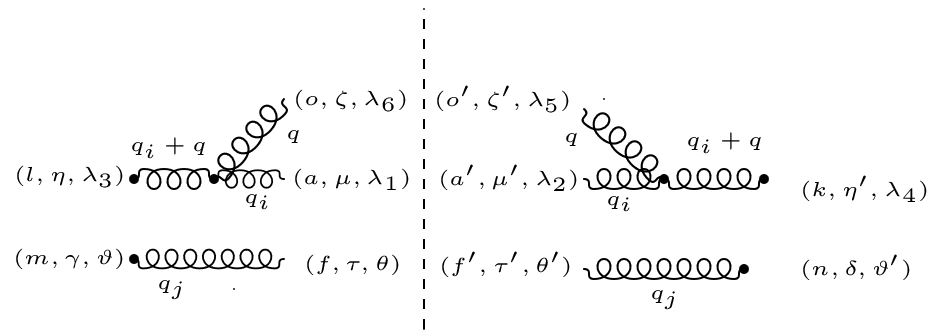
\includegraphics[width=0.95\textwidth]{images/GG/M1Squer.png}
\end{figure}
\begin{equation}
\begin{split}
|M_1|^2=[\frac{-i}{(q_i +q)^2}(-g_s f^{\:a\:o\:l}(g^{{\mu}{\zeta}}(q-q_i)^{\eta}-g^{{\zeta}{\eta}}(2q +q_i)^{\mu}+g^{{\eta}{\mu}}(2q_i +q)^{\zeta})\\
{\varepsilon^{\lambda_1}}_{\mu} (q_i)\:{{\varepsilon^{\lambda_2}}_{{\mu}^{\prime}}}^* (q_i) {\varepsilon^{\lambda_6}}_{\zeta} (q)\:{{\varepsilon^{\lambda_5}}_{{\zeta}^{\prime}}}^* (q)\\
(-g_s f^{\:a^{\prime}\:k\:o^{\prime}}(-g^{{{\mu}^{\prime}}{{\eta}^{\prime}}}(2q_i+q)^{{\zeta}^{\prime}}+g^{{{\eta}^{\prime}}{{\zeta}^{\prime}}}(2q +q_i)^{{\mu}^{\prime}}+g^{{{\zeta}^{\prime}}{{\mu}^{\prime}}}(q_i-q)^{{\eta}^{\prime}})\frac{i}{(q_i +q)^2}][g^{{\gamma}{\delta}}]
\end{split}
\end{equation}

\begin{equation}
\begin{split}
N\equiv g_{{\mu}{{\mu}^{\prime}}} g_{{\zeta}{{\zeta}^{\prime}}}[-g^{{\mu}{\zeta}}g^{{{\mu}^{\prime}}{{\eta}^{\prime}}}(q-q_i)^{{\eta}}(2q_i+q)^{{\zeta}^{\prime}}+g^{{\mu}{\zeta}}g^{{{\eta}^{\prime}}{{\zeta}^{\prime}}}(q-q_i)^{\eta}(2q +q_i)^{{\mu}^{\prime}}\\+g^{{\mu}{\zeta}}g^{{{\zeta}^{\prime}}{{\mu}^{\prime}}}(q-q_i)^{\eta}(q_i -q)^{{\eta}^{\prime}}+g^{{\zeta}{\eta}}g^{{{\mu}^{\prime}}{{\zeta}^{\prime}}}(2q +q_i)^{\mu}(2q_i+q)^{{\zeta}^{\prime}}\\
-g^{{\zeta}{\eta}}g^{{{\eta}^{\prime}}{{\zeta}^{\prime}}}(2q +q_i)^{\mu}(2q +q_i)^{{\mu}^{\prime}}-g^{{\zeta}{\eta}}g^{{{\zeta}^{\prime}}{{\mu}^{\prime}}}(2q +q_i)^{\mu}(q_i -q)^{{\eta}^{\prime}}\\
-g^{{\eta}{\mu}}g^{{{\mu}^{\prime}}{{\eta}^{\prime}}}(2q_i +q)^{\zeta}(2q_i+q)^{{\zeta}^{\prime}}+g^{{\eta}{\mu}}g^{{{\eta}^{\prime}}{{\zeta}^{\prime}}}(2q_i +q)^{\zeta}(2q +q_i)^{{\mu}^{\prime}}\\
+g^{{\eta}{\mu}}g^{{{\zeta}^{\prime}}{{\mu}^{\prime}}}(2q_i +q)^{\zeta}(q_i -q)^{{\eta}^{\prime}}][g^{{\gamma}{\delta}}]
\end{split}
\end{equation}


\begin{equation}
\begin{split}
N\equiv [-(q-q_i)^{{\eta}}(2q_i+q)^{{\eta}^{\prime}}+(q-q_i)^{\eta}(2q +q_i)^{{\eta}^{\prime}}+d(q-q_i)^{\eta}(q_i -q)^{{\eta}^{\prime}}\\+(2q +q_i)^{{\eta}^{\prime}}(2q_i+q)^{{\eta}}
-g^{{\eta}{{\eta}^{\prime}}}(2q +q_i)^{\mu}(2q +q_i)_{{\mu}}-(2q +q_i)^{\eta}(q_i -q)^{{\eta}^{\prime}}\\
-g^{{\eta}{{\eta}^{\prime}}}(2q_i +q)^{\zeta}(2q_i+q)_{{\zeta}}+(2q_i +q)^{{\eta}^{\prime}}(2q +q_i)^{{\eta}}
+(2q_i +q)^{\eta}(q_i -q)^{{\eta}^{\prime}}][g^{{\gamma}{\delta}}]
\end{split}
\end{equation}

\begin{equation}
\begin{split}
N\equiv [-({q}^{{\eta}}{q}^{{\eta}^{\prime}}+2{q}^{{\eta}}{q_i}^{{\eta}^{\prime}}-{q_i}^{{\eta}}{q}^{{\eta}^{\prime}}-2{q_i}^{{\eta}}{q_i}^{{\eta}^{\prime}})
+(2{q}^{{\eta}}{q}^{{\eta}^{\prime}}+{q}^{{\eta}}{q_i}^{{\eta}^{\prime}}-2{q_i}^{{\eta}}{q}^{{\eta}^{\prime}}-{q_i}^{{\eta}}{q_i}^{{\eta}^{\prime}})\\+(d{q}^{{\eta}}{q_i}^{{\eta}^{\prime}}-d{q}^{{\eta}}{q}^{{\eta}^{\prime}}-d{q_i}^{{\eta}}{q_i}^{{\eta}^{\prime}}+d{q_i}^{{\eta}}{q}^{{\eta}^{\prime}})+(4{q}^{{\eta}^{\prime}}{q_i}^{{\eta}}+2{q}^{{\eta}^{\prime}}{q}^{{\eta}}+2{q_i}^{{\eta}^{\prime}}{q_i}^{{\eta}}+{q_i}^{{\eta}^{\prime}}{q}^{{\eta}})\\
-(-2{q}^{{\eta}}{q}^{{\eta}^{\prime}}+2{q}^{{\eta}}{q_i}^{{\eta}^{\prime}}-{q_i}^{{\eta}}{q}^{{\eta}^{\prime}}+{q_i}^{{\eta}}{q_i}^{{\eta}^{\prime}})+(2{q}^{{\eta}^{\prime}}{q}^{{\eta}}+{q}^{{\eta}^{\prime}}{q_i}^{{\eta}}+4{q_i}^{{\eta}^{\prime}}{q}^{{\eta}}+2{q_i}^{{\eta}^{\prime}}{q_i}^{{\eta}})\\+(-{q}^{{\eta}}{q}^{{\eta}^{\prime}}+{q}^{{\eta}}{q_i}^{{\eta}^{\prime}}-2{q_i}^{{\eta}}{q}^{{\eta}^{\prime}}+2{q_i}^{{\eta}}{q_i}^{{\eta}^{\prime}})
-g^{{\eta}{{\eta}^{\prime}}}(5{q}^2+5{q_i}^2+8qq_i)][g^{{\gamma}{\delta}}]
\end{split}
\end{equation}

\begin{equation}
\begin{split}
N\equiv [(6-d){q}^{{\eta}}{q}^{{\eta}^{\prime}}+(d+3){q}^{{\eta}}{q_i}^{{\eta}^{\prime}}+(d+3){q_i}^{{\eta}}{q}^{{\eta}^{\prime}}+(6-d){q_i}^{{\eta}}{q_i}^{{\eta}^{\prime}}\\
-g^{{\eta}{{\eta}^{\prime}}}(5{q}^2+5{q_i}^2+8qq_i)][g^{{\gamma}{\delta}}]
\end{split}
\end{equation}

\begin{equation}
\begin{split}
|M_1|^2=\frac{g_s^2 \:f^{\:a\:o\:l}\: f^{\:a\:k\:o}}{(q_i +q)^2 (q_i +q)^2} [(6-d){q}^{{\eta}}{q}^{{\eta}^{\prime}}+(d+3){q}^{{\eta}}{q_i}^{{\eta}^{\prime}}+(d+3){q_i}^{{\eta}}{q}^{{\eta}^{\prime}}+(6-d){q_i}^{{\eta}}{q_i}^{{\eta}^{\prime}}\\
-g^{{\eta}{{\eta}^{\prime}}}(5{q}^2+5{q_i}^2+8qq_i)][g^{{\gamma}{\delta}}]
\end{split}
\end{equation}


\pagebreak
\subsection{One-loop corrections to the gluon self-energy diagram(Gluon-Emitter Bubble)}
\begin{figure}[h!]
\centering
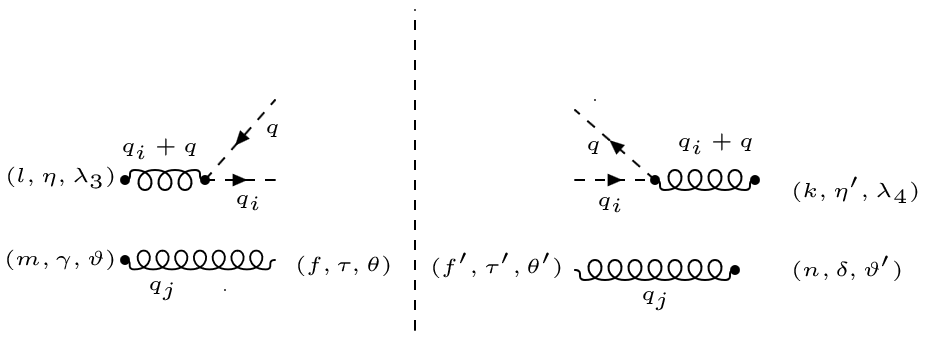
\includegraphics[width=0.95\textwidth]{images/GG/Ghost.png}
\end{figure}

\begin{equation}
\begin{split}
{{|M_1|}^2_{Ghost \:loop}}=\frac{g_s^2 \:f^{\:a\:o\:l}\: f^{\:a\:k\:o}}{(q_i +q)^2 (q_i +q)^2} [-{q_i}^{{\eta}}{q}^{{\eta}^{\prime}}-{q}^{{\eta}}{q_i}^{{\eta}^{\prime}}][g^{{\gamma}{\delta}}]
\end{split}
\end{equation}

\begin{equation}
\begin{split}
{|{M}^{\prime}_1|}^2 = {|M_1|}^2+{{|M_1|}^2_{Ghost \:loop}}\\=\frac{g_s^2 \:f^{\:a\:o\:l}\: f^{\:a\:k\:o}}{(q_i +q)^2 (q_i +q)^2}  [(6-d){q}^{{\eta}}{q}^{{\eta}^{\prime}}+(d+3){q}^{{\eta}}{q_i}^{{\eta}^{\prime}}\\+(d+3){q_i}^{{\eta}}{q}^{{\eta}^{\prime}}+(6-d){q_i}^{{\eta}}{q_i}^{{\eta}^{\prime}}-g^{{\eta}{{\eta}^{\prime}}}(5{q}^2+5{q_i}^2+8qq_i)-{q_i}^{{\eta}}{q}^{{\eta}^{\prime}}-{q}^{{\eta}}{q_i}^{{\eta}^{\prime}}][g^{{\gamma}{\delta}}]
\end{split}
\end{equation}

\begin{equation}
\begin{split}
{|{M}^{\prime}_1|}^2 =\frac{g_s^2 \:f^{\:a\:o\:l}\: f^{\:a\:k\:o}}{(q_i +q)^2 (q_i +q)^2}  [(6-d){q}^{{\eta}}{q}^{{\eta}^{\prime}}+(d+2){q}^{{\eta}}{q_i}^{{\eta}^{\prime}}\\+(d+2){q_i}^{{\eta}}{q}^{{\eta}^{\prime}}+(6-d){q_i}^{{\eta}}{q_i}^{{\eta}^{\prime}}-g^{{\eta}{{\eta}^{\prime}}}(8qq_i)][g^{{\gamma}{\delta}}]
\end{split}
\end{equation}

\begin{equation}
\begin{split}
{|{M}^{\prime}_1|}^2 =\frac{g_s^2 \:f^{\:a\:o\:l}\: f^{\:a\:k\:o}}{4y^2({\alpha_1}+\beta_1)^2\:(p_i\cdot Q) \:(p_i\cdot Q)} \\
[(6-d)(\zeta_1 {p_i}^{\eta} + \lambda_1{Q}^{\eta} + \sqrt{y\alpha_1\beta_1}{n^{\eta}}_{\bot,1})(\zeta_1 {p_i}^{{\eta}^{\prime}} + \lambda_1{Q}^{{\eta}^{\prime}} + \sqrt{y\alpha_1\beta_1}{n^{{\eta}^{\prime}}}_{\bot,1})\\
+(d+2)(\zeta_1 {p_i}^{\eta} + \lambda_1{Q}^{\eta} + \sqrt{y\alpha_1\beta_1}{n^{\eta}}_{\bot,1})(\zeta_q {p_i}^{{\eta}^{\prime}} + \lambda_q{Q}^{{\eta}^{\prime}} - \sqrt{y\alpha_1\beta_1}{n^{{\eta}^{\prime}}}_{\bot,1})\\
+(d+2)(\zeta_q {p_i}^{\eta} + \lambda_q{Q}^{\eta} - \sqrt{y\alpha_1\beta_1}{n^{\eta}}_{\bot,1})(\zeta_1 {p_i}^{{\eta}^{\prime}} + \lambda_1{Q}^{{\eta}^{\prime}} + \sqrt{y\alpha_1\beta_1}{n^{{\eta}^{\prime}}}_{\bot,1})\\
+(6-d)(\zeta_q {p_i}^{\eta} + \lambda_q{Q}^{\eta} - \sqrt{y\alpha_1\beta_1}{n^{\eta}}_{\bot,1})(\zeta_q {p_i}^{{\eta}^{\prime}} + \lambda_q{Q}^{{\eta}^{\prime}} - \sqrt{y\alpha_1\beta_1}{n^{{\eta}^{\prime}}}_{\bot,1})\\
-8g^{{\eta}{{\eta}^{\prime}}}[({\alpha_1}^2+{\beta_1}^2) p_i \cdot Q - ({\beta_1}(1-\beta_1)){n}_{\bot,1}\cdot{n}_{\bot,1}]][g^{{\gamma}{{\delta}}}]
\end{split}
\end{equation}

\begin{equation}
\begin{split}
{|{M}^{\prime}_1|}^2 =\frac{g_s^2 \:f^{\:a\:o\:l}\: f^{\:a\:k\:o}}{y^2\:(p_i\cdot Q) \:(p_i\cdot Q)} \\
[(6-d)[\zeta_1 \zeta_1 {p_i}^{\eta}{p_i}^{{\eta}^{\prime}}+\zeta_1 \lambda_1{p_i}^{\eta}{Q}^{{\eta}^{\prime}}+\zeta_1\sqrt{y\alpha_1\beta_1}{p_i}^{\eta}{n^{{\eta}^{\prime}}}_{\bot,1}\\
+\lambda_1\zeta_1 {Q}^{\eta}{p_i}^{{\eta}^{\prime}}+\lambda_1\lambda_1{Q}^{\eta}{Q}^{{\eta}^{\prime}}+\lambda_1\sqrt{y\alpha_1\beta_1}{Q}^{\eta}{n^{{\eta}^{\prime}}}_{\bot,1}\\
+\zeta_1\sqrt{y\alpha_1\beta_1} {n^{{\eta}}}_{\bot,1}{p_i}^{{\eta}^{\prime}}+\lambda_1\sqrt{y\alpha_1\beta_1}{n^{{\eta}}}_{\bot,1}{Q}^{{\eta}^{\prime}}+\sqrt{y\alpha_1\beta_1}\sqrt{y\alpha_1\beta_1}{n^{{\eta}}}_{\bot,1}{n^{{\eta}^{\prime}}}_{\bot,1}]\\
[(d+2)[\zeta_1 \zeta_q {p_i}^{\eta}{p_i}^{{\eta}^{\prime}}+\zeta_1 \lambda_q{p_i}^{\eta}{Q}^{{\eta}^{\prime}}-\zeta_1\sqrt{y\alpha_1\beta_1}{p_i}^{\eta}{n^{{\eta}^{\prime}}}_{\bot,1}\\
+\lambda_1\zeta_q {Q}^{\eta}{p_i}^{{\eta}^{\prime}}+\lambda_1\lambda_q{Q}^{\eta}{Q}^{{\eta}^{\prime}}-\lambda_1\sqrt{y\alpha_1\beta_1}{Q}^{\eta}{n^{{\eta}^{\prime}}}_{\bot,1}\\
+\zeta_q\sqrt{y\alpha_1\beta_1} {n^{{\eta}}}_{\bot,1}{p_i}^{{\eta}^{\prime}}+\lambda_q\sqrt{y\alpha_1\beta_1}{n^{{\eta}}}_{\bot,1}{Q}^{{\eta}^{\prime}}-\sqrt{y\alpha_1\beta_1}\sqrt{y\alpha_1\beta_1}{n^{{\eta}}}_{\bot,1}{n^{{\eta}^{\prime}}}_{\bot,1}]\\
[(d+2)[\zeta_q \zeta_1 {p_i}^{\eta}{p_i}^{{\eta}^{\prime}}+\zeta_q \lambda_1{p_i}^{\eta}{Q}^{{\eta}^{\prime}}+\zeta_q\sqrt{y\alpha_1\beta_1}{p_i}^{\eta}{n^{{\eta}^{\prime}}}_{\bot,1}\\
+\lambda_q\zeta_1 {Q}^{\eta}{p_i}^{{\eta}^{\prime}}+\lambda_q\lambda_1{Q}^{\eta}{Q}^{{\eta}^{\prime}}+\lambda_q\sqrt{y\alpha_1\beta_1}{Q}^{\eta}{n^{{\eta}^{\prime}}}_{\bot,1}\\
-\zeta_1\sqrt{y\alpha_1\beta_1} {n^{{\eta}}}_{\bot,1}{p_i}^{{\eta}^{\prime}}-\lambda_1\sqrt{y\alpha_1\beta_1}{n^{{\eta}}}_{\bot,1}{Q}^{{\eta}^{\prime}}-\sqrt{y\alpha_1\beta_1}\sqrt{y\alpha_1\beta_1}{n^{{\eta}}}_{\bot,1}{n^{{\eta}^{\prime}}}_{\bot,1}]\\
[(6-d)[\zeta_q \zeta_q {p_i}^{\eta}{p_i}^{{\eta}^{\prime}}+\zeta_q \lambda_q{p_i}^{\eta}{Q}^{{\eta}^{\prime}}-\zeta_q\sqrt{y\alpha_1\beta_1}{p_i}^{\eta}{n^{{\eta}^{\prime}}}_{\bot,1}\\
+\lambda_q\zeta_q {Q}^{\eta}{p_i}^{{\eta}^{\prime}}+\lambda_q\lambda_q{Q}^{\eta}{Q}^{{\eta}^{\prime}}-\lambda_q\sqrt{y\alpha_1\beta_1}{Q}^{\eta}{n^{{\eta}^{\prime}}}_{\bot,1}\\
-\zeta_q\sqrt{y\alpha_1\beta_1} {n^{{\eta}}}_{\bot,1}{p_i}^{{\eta}^{\prime}}-\lambda_q\sqrt{y\alpha_1\beta_1}{n^{{\eta}}}_{\bot,1}{Q}^{{\eta}^{\prime}}+\sqrt{y\alpha_1\beta_1}\sqrt{y\alpha_1\beta_1}{n^{{\eta}}}_{\bot,1}{n^{{\eta}^{\prime}}}_{\bot,1}\\
-8g^{{\eta}{{\eta}^{\prime}}}[({\alpha_1}^2+{\beta_1}^2) p_i \cdot Q - ({\beta_1}(1-\beta_1)){n}_{\bot,1}\cdot{n}_{\bot,1}]][g^{{\gamma}{{\delta}}}]
\end{split}
\end{equation}



\begin{equation}
\begin{split}
{|{M}^{\prime}_1|}^2 =\frac{g_s^2 \:f^{\:a\:o\:l}\: f^{\:a\:k\:o}}{4y^2\:(p_i\cdot Q) \:(p_i\cdot Q)} \\
[(6-d)[({\alpha_1}^2 -2y\alpha_1 \beta_1(\frac{Q^2}{2p_i \cdot Q})+y^2{\beta_1}^2(\frac{Q^2}{2p_i \cdot Q})^2) {p_i}^{\eta}{p_i}^{{\eta}^{\prime}}\\+(y\alpha_1\beta_1 -{y^2\beta_1}^2(\frac{Q^2}{2p_i \cdot Q})){p_i}^{\eta}{Q}^{{\eta}^{\prime}}+\zeta_1\sqrt{y\alpha_1\beta_1}{p_i}^{\eta}{n^{{\eta}^{\prime}}}_{\bot,1}\\
+(y\beta_1\alpha_1 -y^2{\beta_1}^2(\frac{Q^2}{2p_i \cdot Q})) {Q}^{\eta}{p_i}^{{\eta}^{\prime}}+y^2{\beta_1}^2{Q}^{\eta}{Q}^{{\eta}^{\prime}}+\lambda_1\sqrt{y\alpha_1\beta_1}{Q}^{\eta}{n^{{\eta}^{\prime}}}_{\bot,1}\\
+\zeta_1\sqrt{y\alpha_1\beta_1} {n^{{\eta}}}_{\bot,1}{p_i}^{{\eta}^{\prime}}+\lambda_1\sqrt{y\alpha_1\beta_1}{n^{{\eta}}}_{\bot,1}{Q}^{{\eta}^{\prime}}+\sqrt{y\alpha_1\beta_1}\sqrt{y\alpha_1\beta_1}{n^{{\eta}}}_{\bot,1}{n^{{\eta}^{\prime}}}_{\bot,1}]\\
[(d+2)[(\alpha_1\beta_1-y({\alpha_1}^2+{\beta_1}^2) (\frac{Q^2}{2p_i \cdot Q})+y^2{\alpha_1}{\beta_1}(\frac{Q^2}{2p_i \cdot Q})^2) {p_i}^{\eta}{p_i}^{{\eta}^{\prime}}\\+(y{\alpha_1}^2 -y^2\beta_1\alpha_1(\frac{Q^2}{2p_i \cdot Q})){p_i}^{\eta}{Q}^{{\eta}^{\prime}}-\zeta_1\sqrt{y\alpha_1\beta_1}{p_i}^{\eta}{n^{{\eta}^{\prime}}}_{\bot,1}\\
+(y{\beta_1}^2 -y^2\alpha_1 \beta_1(\frac{Q^2}{2p_i \cdot Q})) {Q}^{\eta}{p_i}^{{\eta}^{\prime}}+y^2\beta_1\alpha_1{Q}^{\eta}{Q}^{{\eta}^{\prime}}\\-\lambda_1\sqrt{y\alpha_1\beta_1}{Q}^{\eta}{n^{{\eta}^{\prime}}}_{\bot,1}
+\zeta_q\sqrt{y\alpha_1\beta_1} {n^{{\eta}}}_{\bot,1}{p_i}^{{\eta}^{\prime}}\\+\lambda_q\sqrt{y\alpha_1\beta_1}{n^{{\eta}}}_{\bot,1}{Q}^{{\eta}^{\prime}}-\sqrt{y\alpha_1\beta_1}\sqrt{y\alpha_1\beta_1}{n^{{\eta}}}_{\bot,1}{n^{{\eta}^{\prime}}}_{\bot,1}]\\
[(d+2)[(\beta_1\alpha_1-y({\beta_1}^2+{\alpha_1}^2)(\frac{Q^2}{2p_i \cdot Q})+y^2\alpha_1\beta_1 (\frac{Q^2}{2p_i \cdot Q})^2) {p_i}^{\eta}{p_i}^{{\eta}^{\prime}}\\+(y{\beta_1}^2 -y^2\alpha_1 \beta_1(\frac{Q^2}{2p_i \cdot Q})){p_i}^{\eta}{Q}^{{\eta}^{\prime}}+\zeta_q\sqrt{y\alpha_1\beta_1}{p_i}^{\eta}{n^{{\eta}^{\prime}}}_{\bot,1}\\
+(y{\alpha_1}^2 -y^2\alpha_1\beta_1(\frac{Q^2}{2p_i \cdot Q})) {Q}^{\eta}{p_i}^{{\eta}^{\prime}}+y^2\alpha_1\beta_1{Q}^{\eta}{Q}^{{\eta}^{\prime}}\\+\lambda_q\sqrt{y\alpha_1\beta_1}{Q}^{\eta}{n^{{\eta}^{\prime}}}_{\bot,1}\\
-\zeta_1\sqrt{y\alpha_1\beta_1} {n^{{\eta}}}_{\bot,1}{p_i}^{{\eta}^{\prime}}-\lambda_1\sqrt{y\alpha_1\beta_1}{n^{{\eta}}}_{\bot,1}{Q}^{{\eta}^{\prime}}-\sqrt{y\alpha_1\beta_1}\sqrt{y\alpha_1\beta_1}{n^{{\eta}}}_{\bot,1}{n^{{\eta}^{\prime}}}_{\bot,1}]\\
[(6-d)[({\beta_1}^2 -2y\alpha_1\beta_1 (\frac{Q^2}{2p_i \cdot Q})+ y^2{\alpha_1}^2 (\frac{Q^2}{2p_i \cdot Q})^2) {p_i}^{\eta}{p_i}^{{\eta}^{\prime}}\\+(y\beta_1\alpha_1 -y^2{\alpha_1}^2(\frac{Q^2}{2p_i \cdot Q})){p_i}^{\eta}{Q}^{{\eta}^{\prime}}-\zeta_q\sqrt{y\alpha_1\beta_1}{p_i}^{\eta}{n^{{\eta}^{\prime}}}_{\bot,1}\\
+(y\alpha_1\beta_1 -y^2{\alpha_1}^2 (\frac{Q^2}{2p_i \cdot Q})) {Q}^{\eta}{p_i}^{{\eta}^{\prime}}+y^2{\alpha_1}^2{Q}^{\eta}{Q}^{{\eta}^{\prime}}-\lambda_q\sqrt{y\alpha_1\beta_1}{Q}^{\eta}{n^{{\eta}^{\prime}}}_{\bot,1}\\
-\zeta_q\sqrt{y\alpha_1\beta_1} {n^{{\eta}}}_{\bot,1}{p_i}^{{\eta}^{\prime}}-\lambda_q\sqrt{y\alpha_1\beta_1}{n^{{\eta}}}_{\bot,1}{Q}^{{\eta}^{\prime}}\\+\sqrt{y\alpha_1\beta_1}\sqrt{y\alpha_1\beta_1}{n^{{\eta}}}_{\bot,1}{n^{{\eta}^{\prime}}}_{\bot,1}-8g^{{\eta}{{\eta}^{\prime}}}[({\alpha_1}^2+{\beta_1}^2) p_i \cdot Q - ({\beta_1}(1-\beta_1)){n}_{\bot,1}\cdot{n}_{\bot,1}]][g^{{\gamma}{{\delta}}}]
\end{split}
\end{equation}


\begin{equation}
\begin{split}
{|{M}^{\prime}_1|}^2 =\frac{g_s^2 \:f^{\:a\:o\:l}\: f^{\:a\:k\:o}}{4y^2\:(p_i\cdot Q) \:(p_i\cdot Q)} \\
[(6-d)\lbrace({\alpha_1}^2 -2y\alpha_1 \beta_1(\frac{Q^2}{2p_i \cdot Q})) {p_i}^{\eta}{p_i}^{{\eta}^{\prime}}+y\alpha_1\beta_1 {p_i}^{\eta}{Q}^{{\eta}^{\prime}}+\zeta_1\sqrt{y\alpha_1\beta_1}{p_i}^{\eta}{n^{{\eta}^{\prime}}}_{\bot,1}\\
+y\beta_1\alpha_1  {Q}^{\eta}{p_i}^{{\eta}^{\prime}}+\lambda_1\sqrt{y\alpha_1\beta_1}{Q}^{\eta}{n^{{\eta}^{\prime}}}_{\bot,1}
+\zeta_1\sqrt{y\alpha_1\beta_1} {n^{{\eta}}}_{\bot,1}{p_i}^{{\eta}^{\prime}}+\lambda_1\sqrt{y\alpha_1\beta_1}{n^{{\eta}}}_{\bot,1}{Q}^{{\eta}^{\prime}}\\+y\alpha_1\beta_1{n^{{\eta}}}_{\bot,1}{n^{{\eta}^{\prime}}}_{\bot,1}\rbrace
+(d+2)\lbrace(\alpha_1\beta_1-y({\alpha_1}^2+{\beta_1}^2) (\frac{Q^2}{2p_i \cdot Q})) {p_i}^{\eta}{p_i}^{{\eta}^{\prime}}+y{\alpha_1}^2{p_i}^{\eta}{Q}^{{\eta}^{\prime}}\\-\zeta_1\sqrt{y\alpha_1\beta_1}{p_i}^{\eta}{n^{{\eta}^{\prime}}}_{\bot,1}
+y{\beta_1}^2 {Q}^{\eta}{p_i}^{{\eta}^{\prime}}-\lambda_1\sqrt{y\alpha_1\beta_1}{Q}^{\eta}{n^{{\eta}^{\prime}}}_{\bot,1}
+\zeta_q\sqrt{y\alpha_1\beta_1} {n^{{\eta}}}_{\bot,1}{p_i}^{{\eta}^{\prime}}\\+\lambda_q\sqrt{y\alpha_1\beta_1}{n^{{\eta}}}_{\bot,1}{Q}^{{\eta}^{\prime}}-y\alpha_1\beta_1{n^{{\eta}}}_{\bot,1}{n^{{\eta}^{\prime}}}_{\bot,1}\rbrace\\
+(d+2)\lbrace(\beta_1\alpha_1-y({\beta_1}^2+{\alpha_1}^2)(\frac{Q^2}{2p_i \cdot Q})) {p_i}^{\eta}{p_i}^{{\eta}^{\prime}}+y{\beta_1}^2{p_i}^{\eta}{Q}^{{\eta}^{\prime}}+\zeta_q\sqrt{y\alpha_1\beta_1}{p_i}^{\eta}{n^{{\eta}^{\prime}}}_{\bot,1}\\
+y{\alpha_1}^2 {Q}^{\eta}{p_i}^{{\eta}^{\prime}}+\lambda_q\sqrt{y\alpha_1\beta_1}{Q}^{\eta}{n^{{\eta}^{\prime}}}_{\bot,1}
-\zeta_1\sqrt{y\alpha_1\beta_1} {n^{{\eta}}}_{\bot,1}{p_i}^{{\eta}^{\prime}}-\lambda_1\sqrt{y\alpha_1\beta_1}{n^{{\eta}}}_{\bot,1}{Q}^{{\eta}^{\prime}}\\-y\alpha_1\beta_1{n^{{\eta}}}_{\bot,1}{n^{{\eta}^{\prime}}}_{\bot,1}\rbrace
+(6-d)\lbrace({\beta_1}^2 -2y\alpha_1\beta_1 (\frac{Q^2}{2p_i \cdot Q})) {p_i}^{\eta}{p_i}^{{\eta}^{\prime}}+y\beta_1\alpha_1 {p_i}^{\eta}{Q}^{{\eta}^{\prime}}\\-\zeta_q\sqrt{y\alpha_1\beta_1}{p_i}^{\eta}{n^{{\eta}^{\prime}}}_{\bot,1}
+y\alpha_1\beta_1 {Q}^{\eta}{p_i}^{{\eta}^{\prime}}-\lambda_q\sqrt{y\alpha_1\beta_1}{Q}^{\eta}{n^{{\eta}^{\prime}}}_{\bot,1}
-\zeta_q\sqrt{y\alpha_1\beta_1} {n^{{\eta}}}_{\bot,1}{p_i}^{{\eta}^{\prime}}\\-\lambda_q\sqrt{y\alpha_1\beta_1}{n^{{\eta}}}_{\bot,1}{Q}^{{\eta}^{\prime}}+y\alpha_1\beta_1{n^{{\eta}}}_{\bot,1}{n^{{\eta}^{\prime}}}_{\bot,1}\rbrace-8g^{{\eta}{{\eta}^{\prime}}}[({\alpha_1}^2+{\beta_1}^2) p_i \cdot Q - ({\beta_1}(1-\beta_1)){n}_{\bot,1}\cdot{n}_{\bot,1}]][g^{{\gamma}{{\delta}}}]
\end{split}
\end{equation}


\begin{equation}
\begin{split}
{|{M}^{\prime}_1|}^2 =\frac{g_s^2 \:f^{\:a\:o\:l}\: f^{\:a\:k\:o}}{4y^2\:(p_i\cdot Q) \:(p_i\cdot Q)} \\
[(6-d)\lbrace({\alpha_1}^2 -2y\alpha_1 \beta_1(\frac{Q^2}{2p_i \cdot Q})) {p_i}^{\eta}{p_i}^{{\eta}^{\prime}}+y\alpha_1\beta_1 {p_i}^{\eta}{Q}^{{\eta}^{\prime}}
+y\beta_1\alpha_1  {Q}^{\eta}{p_i}^{{\eta}^{\prime}}\\+y\alpha_1\beta_1{n^{{\eta}}}_{\bot,1}{n^{{\eta}^{\prime}}}_{\bot,1}\rbrace\\
+(d+2)\lbrace(\alpha_1\beta_1-y({\alpha_1}^2+{\beta_1}^2) (\frac{Q^2}{2p_i \cdot Q})) {p_i}^{\eta}{p_i}^{{\eta}^{\prime}}+y{\alpha_1}^2{p_i}^{\eta}{Q}^{{\eta}^{\prime}}+y{\beta_1}^2 {Q}^{\eta}{p_i}^{{\eta}^{\prime}}\\-y\alpha_1\beta_1{n^{{\eta}}}_{\bot,1}{n^{{\eta}^{\prime}}}_{\bot,1}\rbrace+(d+2)\lbrace(\beta_1\alpha_1-y({\beta_1}^2+{\alpha_1}^2)(\frac{Q^2}{2p_i \cdot Q})) {p_i}^{\eta}{p_i}^{{\eta}^{\prime}}+y{\beta_1}^2{p_i}^{\eta}{Q}^{{\eta}^{\prime}}\\
+y{\alpha_1}^2 {Q}^{\eta}{p_i}^{{\eta}^{\prime}}-y\alpha_1\beta_1{n^{{\eta}}}_{\bot,1}{n^{{\eta}^{\prime}}}_{\bot,1}\rbrace
+(6-d)\lbrace({\beta_1}^2 -2y\alpha_1\beta_1 (\frac{Q^2}{2p_i \cdot Q})) {p_i}^{\eta}{p_i}^{{\eta}^{\prime}}\\+y\beta_1\alpha_1 {p_i}^{\eta}{Q}^{{\eta}^{\prime}}
+y\alpha_1\beta_1 {Q}^{\eta}{p_i}^{{\eta}^{\prime}}+y\alpha_1\beta_1{n^{{\eta}}}_{\bot,1}{n^{{\eta}^{\prime}}}_{\bot,1}\rbrace-8g^{{\eta}{{\eta}^{\prime}}}[({\alpha_1}^2+{\beta_1}^2) p_i \cdot Q - ({\beta_1}(1-\beta_1)){n}_{\bot,1}\cdot{n}_{\bot,1}]][g^{{\gamma}{{\delta}}}]
\end{split}
\end{equation}


\begin{equation}
\begin{split}
{|{M}^{\prime}_1|}^2 =\frac{g_s^2 \:f^{\:a\:o\:l}\: f^{\:a\:k\:o}}{4y^2\:(p_i\cdot Q) \:(p_i\cdot Q)} \\
[(6-d)({\alpha_1}^2 -2y\alpha_1 \beta_1(\frac{Q^2}{2p_i \cdot Q}))+2(d+2)({\alpha_1}{\beta}_1 -y({\alpha_1}^2 +{\beta_1}^2)(\frac{Q^2}{2p_i \cdot Q}))\\+(6-d)({\beta_1}^2 -2y\alpha_1 \beta_1(\frac{Q^2}{2p_i \cdot Q})) ]{p_i}^{\eta}{p_i}^{{\eta}^{\prime}}\\
+[2(6-d)y\alpha_1\beta_1+(d+2)y({\alpha_1}^2 +{\beta_1}^2)] {p_i}^{\eta}{Q}^{{\eta}^{\prime}}\\
+[2(6-d)y\beta_1\alpha_1+(d+2)y({\alpha_1}^2 +{\beta_1}^2)]  {Q}^{\eta}{p_i}^{{\eta}^{\prime}}\\+[2(6-d)-2(d+2)]y\alpha_1\beta_1{n^{{\eta}}}_{\bot,1}{n^{{\eta}^{\prime}}}_{\bot,1}-8g^{{\eta}{{\eta}^{\prime}}}[({\alpha_1}^2+{\beta_1}^2) p_i \cdot Q - ({\beta_1}(1-\beta_1)){n}_{\bot,1}\cdot{n}_{\bot,1}][g^{{\gamma}{{\delta}}}]]
\end{split}
\end{equation}

\begin{equation}
\begin{split}
{|{M}^{\prime}_1|}^2 =\frac{g_s^2 \:f^{\:a\:o\:l}\: f^{\:a\:k\:o}}{4y^2\:(p_i\cdot Q) \:(p_i\cdot Q)} \\
[(6-d)({\alpha_1}^2 -2y\alpha_1 \beta_1(\frac{Q^2}{2p_i \cdot Q}))+2(d+2)({\alpha_1}{\beta}_1 -y({\alpha_1}^2 +{\beta_1}^2)(\frac{Q^2}{2p_i \cdot Q}))\\+(6-d)({\beta_1}^2 -2y\alpha_1 \beta_1(\frac{Q^2}{2p_i \cdot Q})) ]{p_i}^{\eta}{p_i}^{{\eta}^{\prime}}\\
+y[(4d-8){\alpha_1}^2+(8-4d){\alpha}_1 +(d+2)] {p_i}^{\eta}{Q}^{{\eta}^{\prime}}\\
+y[(4d-8){\alpha_1}^2+(8-4d){\alpha}_1 +(d+2)]  {Q}^{\eta}{p_i}^{{\eta}^{\prime}}\\+y[8-4d](\alpha_1-{\alpha_1}^2){n^{{\eta}}}_{\bot,1}{n^{{\eta}^{\prime}}}_{\bot,1}-8g^{{\eta}{{\eta}^{\prime}}}[({\alpha_1}^2+{\beta_1}^2) p_i \cdot Q - ({\beta_1}(1-\beta_1)){n}_{\bot,1}\cdot{n}_{\bot,1}][g^{{\gamma}{{\delta}}}]]
\end{split}
\end{equation}

\begin{equation}
\begin{split}
{|{M}^{\prime}_1|}^2 =\frac{g_s^2 \:f^{\:a\:o\:l}\: f^{\:a\:k\:o}}{4y\:(p_i\cdot Q) \:(p_i\cdot Q)} \\
[[8-4d]{\beta_1}(1-\beta_1){n^{{\eta}}}_{\bot,1}{n^{{\eta}^{\prime}}}_{\bot,1}-8g^{{\eta}{{\eta}^{\prime}}}[({\alpha_1}^2+{\beta_1}^2) p_i \cdot Q - ({\beta_1}(1-\beta_1)){n}_{\bot,1}\cdot{n}_{\bot,1}][g^{{\gamma}{{\delta}}}]]
\end{split}
\end{equation}

\begin{equation}
\begin{split}
{|{M}^{\prime}_1|}^2 =\frac{g_s^2 \:f^{\:a\:o\:l}\: f^{\:a\:k\:o}}{4y\:(p_i\cdot Q) \:(p_i\cdot Q)} \\
[8[\epsilon-1]{\beta_1}(1-\beta_1){n^{{\eta}}}_{\bot,1}{n^{{\eta}^{\prime}}}_{\bot,1}-8g^{{\eta}{{\eta}^{\prime}}}[({\alpha_1}^2+{\beta_1}^2) p_i \cdot Q - ({\beta_1}(1-\beta_1))(-2p_i \cdot Q)][g^{{\gamma}{{\delta}}}]]
\end{split}
\end{equation}

\begin{equation}
\begin{split}
{|{M}^{\prime}_1|}^2 =\frac{g_s^2 \:f^{\:a\:o\:l}\: f^{\:a\:k\:o}}{4y\:(p_i\cdot Q) \:(p_i\cdot Q)} \\
[8[\epsilon-1]{\beta_1}(1-\beta_1){n^{{\eta}}}_{\bot,1}{n^{{\eta}^{\prime}}}_{\bot,1}-8g^{{\eta}{{\eta}^{\prime}}}[({\alpha_1}^2+{\beta_1}^2) p_i \cdot Q +2{\alpha_1}{\beta_1} p_i \cdot Q)][g^{{\gamma}{{\delta}}}]]
\end{split}
\end{equation}

\begin{equation}
\begin{split}
{|{M}^{\prime}_1|}^2 =\frac{g_s^2 \:f^{\:a\:o\:l}\: f^{\:a\:k\:o}}{4y\:(p_i\cdot Q) \:(p_i\cdot Q)} \\
[8[\epsilon-1]{\beta_1}(1-\beta_1){n^{{\eta}}}_{\bot,1}{n^{{\eta}^{\prime}}}_{\bot,1}-8g^{{\eta}{{\eta}^{\prime}}}[({\alpha_1}+{\beta_1})^2 p_i \cdot Q)][g^{{\gamma}{{\delta}}}]]
\end{split}
\end{equation}

\begin{equation}
\begin{split}
{|{M}^{\prime}_1|}^2 =\frac{g_s^2 \:f^{\:a\:o\:l}\: f^{\:a\:k\:o}}{y\:(p_i\cdot Q)}[-2g^{{\eta}{{\eta}^{\prime}}}][g^{{\gamma}{{\delta}}}]]
\end{split}
\end{equation}

\pagebreak

Another way:
\begin{equation}
\begin{split}
{k_1}^{{\eta}}{k_1}^{{\eta}^{\prime}}&=({\alpha_1}^2 -2\alpha_1 \beta_1 y(\frac{Q^2}{2 p_i \cdot Q})){p_i}^{{\eta}}{p_i}^{{\eta}^{\prime}}+y\alpha_1 \beta_1 {p_i}^{{\eta}}{Q}^{{\eta}^{\prime}}+y\alpha_1 \beta_1 {Q}^{{\eta}}{p_i}^{{\eta}^{\prime}}+y\alpha_1\beta_1 {n}^{{\eta}}_{\bot,1}{n}^{{\eta}^{\prime}}_{\bot,1}\\
{k_1}^{{\eta}}{q_i}^{{\eta}^{\prime}}&=({\alpha_1}\beta_1 -y({\alpha_1}^2 + {\beta_1}^2 )(\frac{Q^2}{2 p_i \cdot Q})){p_i}^{{\eta}}{p_i}^{{\eta}^{\prime}}+y{\alpha_1}^2 {p_i}^{{\eta}}{Q}^{{\eta}^{\prime}}+y{\beta_1}^2 {Q}^{{\eta}}{p_i}^{{\eta}^{\prime}}-y\alpha_1\beta_1 {n}^{{\eta}}_{\bot,1}{n}^{{\eta}^{\prime}}_{\bot,1}\\
{q_i}^{{\eta}}{k_1}^{{\eta}^{\prime}}&=({\alpha_1}\beta_1 -y({\alpha_1}^2 + {\beta_1}^2 )(\frac{Q^2}{2 p_i \cdot Q})){p_i}^{{\eta}}{p_i}^{{\eta}^{\prime}}+y{\beta_1}^2 {p_i}^{{\eta}}{Q}^{{\eta}^{\prime}}+y{\alpha_1}^2 {Q}^{{\eta}}{p_i}^{{\eta}^{\prime}}-y\alpha_1\beta_1 {n}^{{\eta}}_{\bot,1}{n}^{{\eta}^{\prime}}_{\bot,1}\\
{q_i}^{{\eta}}{q_i}^{{\eta}^{\prime}}&=({\beta_1}^2 -2\alpha_1 \beta_1 y(\frac{Q^2}{2 p_i \cdot Q})){p_i}^{{\eta}}{p_i}^{{\eta}^{\prime}}+y\alpha_1 \beta_1 {p_i}^{{\eta}}{Q}^{{\eta}^{\prime}}+y\alpha_1 \beta_1 {Q}^{{\eta}}{p_i}^{{\eta}^{\prime}}+y\alpha_1\beta_1 {n}^{{\eta}}_{\bot,1}{n}^{{\eta}^{\prime}}_{\bot,1}
\end{split}
\end{equation}

\begin{equation}
\begin{split}
N\equiv&(6-d)({\alpha_1}^2 -2\alpha_1 \beta_1 y(\frac{Q^2}{2 p_i \cdot Q})){p_i}^{{\eta}}{p_i}^{{\eta}^{\prime}}+y\alpha_1 \beta_1 {p_i}^{{\eta}}{Q}^{{\eta}^{\prime}}+y\alpha_1 \beta_1 {Q}^{{\eta}}{p_i}^{{\eta}^{\prime}}+y\alpha_1\beta_1 {n}^{{\eta}}_{\bot,1}{n}^{{\eta}^{\prime}}_{\bot,1}\\
&+(d+2)({\alpha_1}\beta_1 -y({\alpha_1}^2 + {\beta_1}^2 )(\frac{Q^2}{2 p_i \cdot Q})){p_i}^{{\eta}}{p_i}^{{\eta}^{\prime}}+y{\alpha_1}^2 {p_i}^{{\eta}}{Q}^{{\eta}^{\prime}}+y{\beta_1}^2 {Q}^{{\eta}}{p_i}^{{\eta}^{\prime}}-y\alpha_1\beta_1 {n}^{{\eta}}_{\bot,1}{n}^{{\eta}^{\prime}}_{\bot,1}\\
&+(d+2)({\alpha_1}\beta_1 -y({\alpha_1}^2 + {\beta_1}^2 )(\frac{Q^2}{2 p_i \cdot Q})){p_i}^{{\eta}}{p_i}^{{\eta}^{\prime}}+y{\beta_1}^2 {p_i}^{{\eta}}{Q}^{{\eta}^{\prime}}+y{\alpha_1}^2 {Q}^{{\eta}}{p_i}^{{\eta}^{\prime}}-y\alpha_1\beta_1 {n}^{{\eta}}_{\bot,1}{n}^{{\eta}^{\prime}}_{\bot,1}\\
&+(6-d)({\beta_1}^2 -2\alpha_1 \beta_1 y(\frac{Q^2}{2 p_i \cdot Q})){p_i}^{{\eta}}{p_i}^{{\eta}^{\prime}}+y\alpha_1 \beta_1 {p_i}^{{\eta}}{Q}^{{\eta}^{\prime}}+y\alpha_1 \beta_1 {Q}^{{\eta}}{p_i}^{{\eta}^{\prime}}+y\alpha_1\beta_1 {n}^{{\eta}}_{\bot,1}{n}^{{\eta}^{\prime}}_{\bot,1}\\
&-8g^{{\eta}{{\eta}^{\prime}}}[({\alpha_1}^2+{\beta_1}^2) p_i \cdot Q - ({\beta_1}(1-\beta_1)){n}_{\bot,1}\cdot{n}_{\bot,1}]\\
\end{split}
\end{equation}

\begin{equation}
\begin{split}
N\equiv&[(6-d)({\alpha_1}^2 -2\alpha_1 \beta_1 y(\frac{Q^2}{2 p_i \cdot Q}))+(d+2)({\alpha_1}\beta_1 -y({\alpha_1}^2 + {\beta_1}^2 )(\frac{Q^2}{2 p_i \cdot Q}))\\&+(d+2)({\alpha_1}\beta_1 -y({\alpha_1}^2 + {\beta_1}^2 )(\frac{Q^2}{2 p_i \cdot Q}))+(6-d)({\beta_1}^2 -2\alpha_1 \beta_1 y(\frac{Q^2}{2 p_i \cdot Q}))]{p_i}^{{\eta}}{p_i}^{{\eta}^{\prime}}\\
&+[(6-d)y\alpha_1 \beta_1+(d+2)y{\alpha_1}^2+(d+2)y{\beta_1}^2+(6-d)y\alpha_1 \beta_1] {p_i}^{{\eta}}{Q}^{{\eta}^{\prime}}\\
&+[(6-d)y\alpha_1 \beta_1 +(d+2)y{\beta_1}^2+(d+2)y{\alpha_1}^2+(6-d)y\alpha_1 \beta_1] {Q}^{{\eta}}{p_i}^{{\eta}^{\prime}}\\
&+[(6-d)y\alpha_1\beta_1-(d+2)y\alpha_1\beta_1-(d+2)y\alpha_1\beta_1+(6-d)y\alpha_1\beta_1] {n}^{{\eta}}_{\bot,1}{n}^{{\eta}^{\prime}}_{\bot,1}\\
&-8g^{{\eta}{{\eta}^{\prime}}}[({\alpha_1}^2+{\beta_1}^2) p_i \cdot Q - ({\beta_1}(1-\beta_1)){n}_{\bot,1}\cdot{n}_{\bot,1}]\\
\end{split}
\end{equation}

\begin{equation}
\begin{split}
&{|{M}^{\prime}_1|}^2 =\frac{g_s^2 \:f^{\:a\:o\:l}\: f^{\:a\:k\:o}}{4y\:(p_i\cdot Q)^2} 
[(12-2d)y\alpha_1\beta_1-2(d+2)y\alpha_1\beta_1] {n}^{{\eta}}_{\bot,1}{n}^{{\eta}^{\prime}}_{\bot,1}-8yg^{{\eta}{{\eta}^{\prime}}} p_i \cdot Q][g_{{\gamma}{{\delta}}}]\\
&\Rightarrow {|{M}^{\prime}_1|}^2 =\frac{g_s^2 \:f^{\:a\:o\:l}\: f^{\:a\:k\:o}}{4y\:(p_i\cdot Q)^2} 
[(12-2d)\alpha_1\beta_1-2(d+2)\alpha_1\beta_1] {n}^{{\eta}}_{\bot,1}{n}^{{\eta}^{\prime}}_{\bot,1}
-8g^{{\eta}{{\eta}^{\prime}}}({\alpha_1}^2+{\beta_1}^2) p_i \cdot Q][g_{{\gamma}{{\delta}}}]\\
& {|{M}^{\prime}_1|}^2 =\frac{g_s^2 \:f^{\:a\:o\:l}\: f^{\:a\:k\:o}}{4y\:(p_i\cdot Q) \:(p_i\cdot Q)}\\
&[8[\epsilon-1]{\beta_1}(1-\beta_1){n^{{\eta}}}_{\bot,1}{n^{{\eta}^{\prime}}}_{\bot,1}-8g^{{\eta}{{\eta}^{\prime}}}[({\alpha_1}^2+{\beta_1}^2) p_i \cdot Q - {\beta_1} \alpha_1(-2p_i \cdot Q)]][g_{{\gamma}{{\delta}}}]
\end{split}
\end{equation}


\begin{equation}
\begin{split}
{|{M}^{\prime}_1|}^2 =\frac{g_s^2 \:f^{\:a\:o\:l}\: f^{\:a\:k\:o}}{y\:(p_i\cdot Q)}[-2g^{{\eta}{{\eta}^{\prime}}}][g^{{\gamma}{{\delta}}}]]
\end{split}
\end{equation}

\pagebreak
\section{Gluon-Spectator Bubble}
\begin{figure}[ht!]
\centering
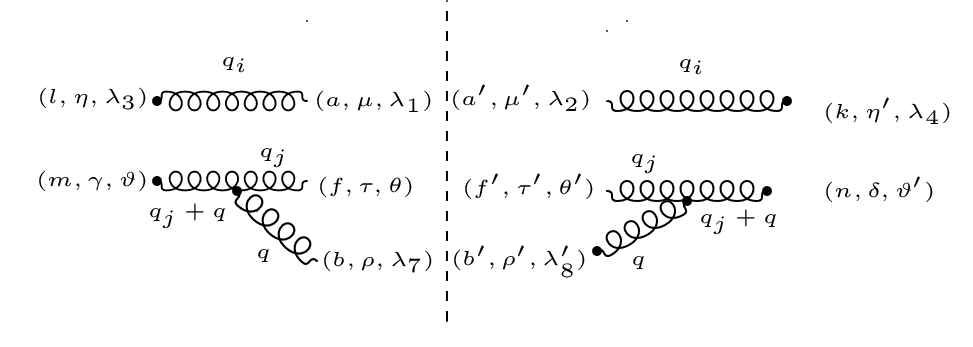
\includegraphics[width=0.95\textwidth]{images/GG/M2Squer}
\end{figure}
\begin{equation}
\begin{split}
|M_2|^2=[\frac{-i}{(q_j +q)^2}(-g_s f^{\:b\:f\:m}(g^{{\tau}{\gamma}}(-2q_j-q)^{\rho}+g^{{\gamma}{\rho}}(2q +q_j)^{\tau}+g^{{\rho}{\tau}}(q_j -q)^{\gamma})\\g_{{\tau}{{\tau}^{\prime}}}g_{{\rho}{{\rho}^{\prime}}}
(-g_s f^{\:b^{\prime}\:n\:f^{\prime}}(g^{{{\rho}^{\prime}}{{\delta}}}(-2q-q_j)^{{\tau}^{\prime}}+g^{{{\delta}}{{\tau}^{\prime}}}(2q_j +q)^{{\rho}^{\prime}}+g^{{{\tau}^{\prime}}{{\rho}^{\prime}}}(q-q_j)^{{\delta}})\frac{i}{(q_j +q)^2}][g^{{\eta}{{\eta}^{\prime}}}]
\end{split}
\end{equation}

\begin{equation}
\begin{split}
|M_2|^2=\frac{g_s^2\: f^{\:b\:f\:m} f^{\:b^{\prime}\:n\:f^{\prime}} {\delta}^{{a}{a^{\prime}}} {\delta}^{{f}{f^{\prime}}} {\delta}^{{b}{b^{\prime}}}}{(q_j +q)^2 (q_j +q)^2}[g_{{\tau}{{\tau}^{\prime}}}g_{{\rho}{{\rho}^{\prime}}}(g^{{\tau}{\gamma}}(2q_j+q)^{\rho}g^{{{\rho}^{\prime}}{{\delta}}}(2q+q_j)^{{\tau}^{\prime}}\\
-g^{{\tau}{\gamma}}(2q_j+q)^{\rho}g^{{{\delta}}{{\tau}^{\prime}}}(2q_j +q)^{{\rho}^{\prime}}-g^{{\tau}{\gamma}}(2q_j+q)^{\rho}g^{{{\tau}^{\prime}}{{\rho}^{\prime}}}(q-q_j)^{{\delta}}-g^{{\gamma}{\rho}}(2q +q_j)^{\tau}g^{{{\rho}^{\prime}}{{\delta}}}(2q+q_j)^{{\tau}^{\prime}}\\
+g^{{\gamma}{\rho}}(2q +q_j)^{\tau}g^{{{\delta}}{{\tau}^{\prime}}}(2q_j +q)^{{\rho}^{\prime}}+g^{{\gamma}{\rho}}(2q +q_j)^{\tau}g^{{{\tau}^{\prime}}{{\rho}^{\prime}}}(q-q_j)^{{\delta}}-g^{{\rho}{\tau}}(q_j -q)^{\gamma}g^{{{\rho}^{\prime}}{{\delta}}}(2q+q_j)^{{\tau}^{\prime}}\\
+g^{{\rho}{\tau}}(q_j -q)^{\gamma}g^{{{\delta}}{{\tau}^{\prime}}}(2q_j +q)^{{\rho}^{\prime}}
+g^{{\rho}{\tau}}(q_j -q)^{\gamma}g^{{{\tau}^{\prime}}{{\rho}^{\prime}}}(q-q_j)^{{\delta}}
][g^{{\eta}{{\eta}^{\prime}}}]
\end{split}
\end{equation}


\begin{equation}
\begin{split}
|M_2|^2=\frac{g_s^2\: f^{\:b\:f\:m} f^{\:b\:n\:f}}{(q_j +q)^2 (q_j +q)^2}[(2q+q_j)^{{\gamma}}(2q_j+q)^{\delta}\\
-g^{{\delta}{\gamma}}(2q_j+q)^{\rho}(2q_j +q)_{{\rho}}-(2q_j+q)^{\gamma}(q-q_j)^{{\delta}}-g^{{\delta}{\gamma}}(2q +q_j)^{\tau}(2q+q_j)_{{\tau}}\\
+(2q_j +q)^{{\gamma}}(2q +q_j)^{\delta}+(2q +q_j)^{\gamma}(q-q_j)^{{\delta}}-(q_j -q)^{\gamma}(2q+q_j)^{{\delta}}\\
+(q_j -q)^{\gamma}(2q_j +q)^{{\delta}}+d(q_j -q)^{\gamma}(q-q_j)^{{\delta}}][g^{{\eta}{{\eta}^{\prime}}}]
\end{split}
\end{equation}


\begin{equation}
\begin{split}
|M_2|^2=\frac{g_s^2\: f^{\:b\:f\:m} f^{\:b\:n\:f}}{(q_j +q)^2 (q_j +q)^2}[(3+d)q^{\gamma}{q_j}^{\delta}+(6-d)q^{\gamma}{q}^{\delta}\\+(6-d){q_j}^{\gamma}{q_j}^{\delta}+(3+d){q_j}^{\gamma}{q}^{\delta}-g^{{\delta}{\gamma}}(5{q_j}^2+5q^2+8qq_j)\\
][g^{{\eta}{{\eta}^{\prime}}}]
\end{split}
\end{equation}





\pagebreak
\subsection{One-loop corrections to the gluon self-energy diagram (Gluon-Spectator Bubble)}
\begin{figure}[h!]
\centering
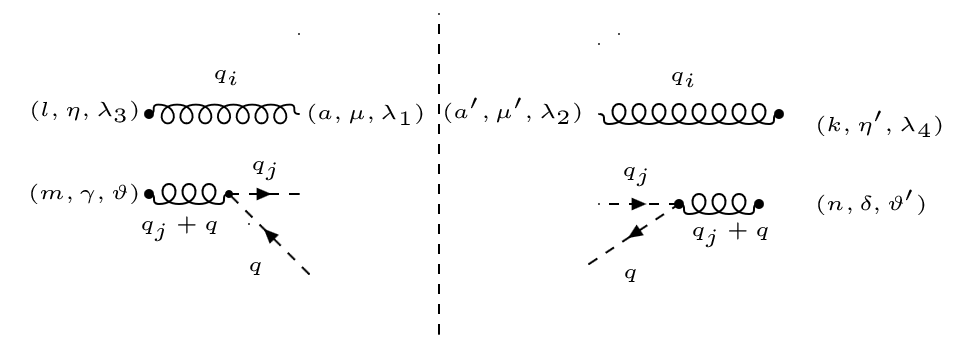
\includegraphics[width=0.95\textwidth]{images/GG/GhostM2.png}
\end{figure}
\begin{equation}
\begin{split}
{{|M_2|}^2_{Ghost \:loop}}=\frac{g_s^2 \:f^{\:b\:f\:m} f^{\:b\:n\:f}}{(q_j +q)^2 (q_j +q)^2} [-{q_j}^{{\gamma}}{q}^{{\delta}}-{q}^{{\delta}}{q_j}^{{\gamma}}][g^{{\eta}{{\eta}^{\prime}}}]
\end{split}
\end{equation}

\begin{equation}
\begin{split}
{|{M}^{\prime}_2|}^2 =\frac{g_s^2\: f^{\:b\:f\:m} f^{\:b\:n\:f}}{(q_j +q)^2 (q_j +q)^2}[(2+d)q^{\gamma}{q_j}^{\delta}+(6-d)q^{\gamma}{q}^{\delta}\\+(6-d){q_j}^{\gamma}{q_j}^{\delta}+(2+d){q_j}^{\gamma}{q}^{\delta}-g^{{\delta}{\gamma}}(8qq_j)][g^{{\eta}{{\eta}^{\prime}}}]
\end{split}
\end{equation}

\begin{equation}
\begin{split}
{|{M}^{\prime}_2|}^2 =\frac{g_s^2\: f^{\:b\:f\:m} f^{\:b\:n\:f}}{4(q_j \cdot q) (q_j \cdot q)}[-8g^{{\delta}{\gamma}}(q \cdot q_j)][g^{{\eta}{{\eta}^{\prime}}}]
\end{split}
\end{equation}

\begin{equation}
\begin{split}
{|{M}^{\prime}_2|}^2 =\frac{g_s^2\: f^{\:b\:f\:m} f^{\:b\:n\:f}}{(q_j \cdot q)}[-2g^{{\delta}{\gamma}}][g^{{\eta}{{\eta}^{\prime}}}]
\end{split}
\end{equation}

\begin{equation}
\begin{split}
{|{M}^{\prime}_2|}^2 =\frac{g_s^2\: f^{\:b\:f\:m} f^{\:b\:n\:f}}{(1-\beta_1) (1-y)\:(p_i \cdot p_k)}[-2g^{{\delta}{\gamma}}][g^{{\eta}{{\eta}^{\prime}}}]
\end{split}
\end{equation}

\section{Interference term $M_1 {M_2}^{\dagger}$}
\begin{figure}[h!]
\centering
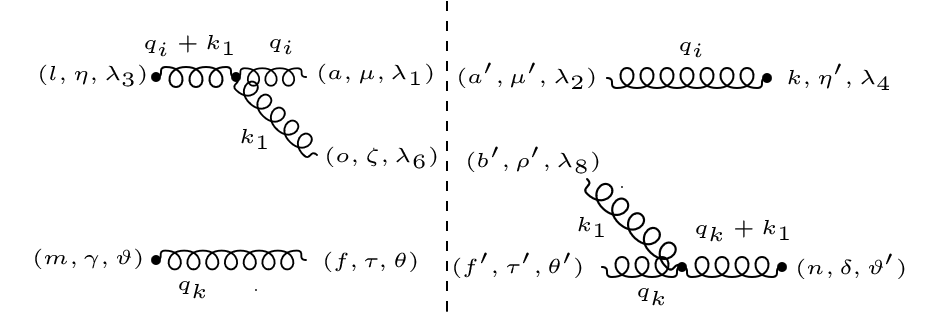
\includegraphics[width=0.95\textwidth]{images/GG/M1M2Dagger.png}
\end{figure}

\begin{equation}
\begin{split}
&M_1{M_2}^{\dagger}=[\frac{-i}{(q_i +q)^2}(-g_s f^{\:l\:a\:o}(g^{{\eta}{\mu}}(2q_i+q)^{\zeta}+g^{{\mu}{\zeta}}(q -q_i)^{\eta}-g^{{\zeta}{\eta}}(2q +q_i)^{\mu}){\varepsilon^{\lambda_1}}_{\mu} (q_i) {\varepsilon^{\lambda_6}}_{\zeta}(q)]\\
&[{{\varepsilon^{\theta}}_{{\tau}}}^* (q_j)]\\
&[\frac{i}{(q +q_j)^2}(-g_s f^{\:f^{\prime}\:b^{\prime}\:n }(g^{{{\tau}^{\prime}}{{\rho}^{\prime}}}(q_j-q)^{{\delta}}+g^{{{\rho}^{\prime}}{{\delta}}}(2q +q_j)^{{\tau}^{\prime}}-g^{{{\delta}}{{\tau}^{\prime}}}(2q_j+q)^{{\rho}^{\prime}}){{\varepsilon^{{\theta}^{\prime}}}_{{\tau}^{\prime}}}^* (q_j){{\varepsilon^{\lambda_8}}_{{\rho}^{\prime}}}^* (q)]\\
&[{{\varepsilon^{\lambda_2}}_{{\mu}^{\prime}}}^* (q_i)]
\end{split}
\end{equation}


\begin{equation}
\begin{split}
&M_1{M_2}^{\dagger}=\frac{g_s^2 f^{\:l\:a\:o} f^{\:f^{\prime}\: b^{\prime}\:n} \delta^{aa^{\prime}} \delta^{ob^{\prime}} \delta^{ff^{\prime}}}{(q_i +q)^2 (q_j +q)^2}
[{g_{{\mu}}}^{{\eta}^{\prime}} g_{{\tau}{{\tau}^{\prime}}}(g^{{\eta}{\mu}}(2q_i+q)^{\zeta}+g^{{\mu}{\zeta}}(q -q_i)^{\eta}-g^{{\zeta}{\eta}}(2q +q_i)^{\mu})\\
&g_{{{\zeta}}{{\rho}^{\prime}}}(g^{{{\tau}^{\prime}}{{\rho}^{\prime}}}(q_j-q)^{{\delta}}+g^{{{\rho}^{\prime}}{{\delta}}}(2q +q_j)^{{\tau}^{\prime}}-g^{{{\delta}}{{\tau}^{\prime}}}(2q_j+q)^{{\rho}^{\prime}}]
\end{split}
\end{equation}


\begin{equation}
\begin{split}
&M_1{M_2}^{\dagger}=\frac{g_s^2 f^{\:l\:a\:o} f^{\:f^{\prime}\: b^{\prime}\:n} \delta^{aa^{\prime}} \delta^{ob^{\prime}}\delta^{ff^{\prime}}}{(q_i +q)^2 (q_j +q)^2}\\
&[g^{{{\eta}}{{\eta}^{\prime}}}(2q_i+q)^{\gamma}(q_j-q)^{{\delta}}+g^{{{\eta}}{{\eta}^{\prime}}}(2q +q_j)^{\gamma}(2q_i+q)^{{\delta}}-g^{{{\eta}}{{\eta}^{\prime}}}g^{{{\gamma}}{{\delta}}}(2q_i+q)\cdot (2q_j+q)\\
&+g^{{{\gamma}}{{\eta}^{\prime}}}(q -q_i)^{\eta}(q_j-q)^{{\delta}}+g^{{{\eta}^{\prime}}{{\delta}}}(q -q_i)^{\eta}(2q +q_j)^{{\gamma}}
-g^{{{\gamma}}{{\delta}}}(q -q_i)^{\eta}(2q_j+q)^{{\eta}^{\prime}}\\
&-g^{{{\gamma}}{{\eta}}}(2q +q_i)^{{\eta}^{\prime}}(q_j-q)^{{\delta}}
-g^{{{\eta}}{{\delta}}}(2q +q_i)^{{\eta}^{\prime}}(2q +q_j)^{{\gamma}}
+g^{{{\gamma}}{{\delta}}}(2q_j+q)^{{\eta}}(2q +q_i)^{{\eta}^{\prime}}]\\
\end{split}
\end{equation}


\begin{equation}
\begin{split}
&M_1{M_2}^{\dagger}=\frac{g_s^2 f^{\:l\:a\:o} f^{\:f\: o\:n}}{4(q \cdot q_i) (q \cdot q_j)}\\
&\lbrace g^{{{\eta}}{{\eta}^{\prime}}}[2{q_i}^{{\gamma}}{q_j}^{\delta}+2{q_i}^{{\gamma}}{q}^{\delta}+{q}^{{\gamma}}{q_j}^{\delta}+{q}^{{\gamma}}{q}^{\delta}+4q^{{\gamma}}{q_i}^{\delta}+2q^{{\gamma}}{q}^{\delta}+2{q_j}^{{\gamma}}{q_i}^{\delta}+{q_j}^{{\gamma}}{q}^{\delta}]\\
&-g^{{{\eta}}{{\eta}^{\prime}}}g^{{{\gamma}}{{\delta}}}(2q\cdot q_j+ q\cdot q+4q_i \cdot q_j+2q_i \cdot q)+g^{{{\gamma}}{{\eta}^{\prime}}}[{q}^{{\eta}}{q_j}^{\delta}-{q}^{{\eta}}{q}^{\delta}-{q_i}^{{\eta}}{q_j}^{\delta}+{q_i}^{{\eta}}{q}^{\delta}]\\
&+g^{{{\eta}^{\prime}}{{\delta}}}[2{q}^{{\eta}}{q}^{\gamma}+{q}^{{\eta}}{q_j}^{\gamma}+{q_i}^{{\eta}}{q}^{\gamma}+{q_i}^{{\eta}}{q_j}^{\gamma}]-g^{{{\gamma}}{{\delta}}}[2{q}^{\eta}{q_j}^{{\eta}^{\prime}}+{q}^{\eta}{q}^{{\eta}^{\prime}}-2{q_i}^{\eta}{q_j}^{{\eta}^{\prime}}-{q_i}^{\eta}{q}^{{\eta}^{\prime}}]\\
&-g^{{{\gamma}}{{\eta}}}[2{q}^{{\eta}^{\prime}}{q_j}^{{\delta}}-{2q}^{{\eta}^{\prime}}{q}^{{\delta}}+{q_i}^{{\eta}^{\prime}}{q_j}^{{\delta}}-{q_i}^{{\eta}^{\prime}}{q}^{{\delta}}]-g^{{{\eta}}{{\delta}}}[4{q}^{{\eta}^{\prime}}{q}^{{\gamma}}+2{q}^{{\eta}^{\prime}}{q_j}^{{\gamma}}+2{q_i}^{{\eta}^{\prime}}{q}^{{\gamma}}+{q_i}^{{\eta}^{\prime}}{q_j}^{{\gamma}}]\\
&+g^{{{\gamma}}{{\delta}}}[4{q_j}^{{\eta}}{q}^{{\eta}^{\prime}}+2{q_j}^{{\eta}}{q_i}^{{\eta}^{\prime}}+{q}^{{\eta}}{q}^{{\eta}^{\prime}}+{q}^{{\eta}}{q_i}^{{\eta}^{\prime}}]\rbrace
\end{split}
\end{equation}



\begin{equation}
\begin{split}
{k_1}^{{\eta}}{k_1}^{{\eta}^{\prime}}&=[(1-\beta_1)^2-y^2 {\beta_1}^2 (\frac{Q^2}{2p_i \cdot Q})^2] {p_i}^{{\eta}}{p_i}^{{\eta}^{\prime}}-y^2 {\beta_1}^2 (\frac{Q^2}{2p_i \cdot Q}){p_i}^{{\eta}}{Q}^{{\eta}^{\prime}}-y^2 {\beta_1}^2 (\frac{Q^2}{2p_i \cdot Q}){Q}^{{\eta}}{p_i}^{{\eta}^{\prime}}\\
{k_1}^{{\eta}}{q_i}^{{\eta}^{\prime}}&=[\beta_1(1-\beta_1)-y {\beta_1}^2 (\frac{Q^2}{2p_i \cdot Q})] {p_i}^{{\eta}}{p_i}^{{\eta}^{\prime}}+y {\beta_1}^2 {Q}^{{\eta}}{p_i}^{{\eta}^{\prime}}\\
{q_i}^{{\eta}}{k_1}^{{\eta}^{\prime}}&=[\beta_1(1-\beta_1)-y {\beta_1}^2 (\frac{Q^2}{2p_i \cdot Q})] {p_i}^{{\eta}}{p_i}^{{\eta}^{\prime}}+y {\beta_1}^2 {p_i}^{{\eta}}{Q}^{{\eta}^{\prime}}\\
{q_i}^{{\eta}}{q_i}^{{\eta}^{\prime}}&={\beta_1}^2 {p_i}^{{\eta}}{p_i}^{{\eta}^{\prime}}\\
{k_1}^{{\eta}}{q_k}^{{\eta}^{\prime}}&= [(1-\beta_1)-y\beta_1 (\frac{Q^2}{2p_i \cdot Q})] \sqrt{1-y}{p_i}^{{\eta}}{{p_k}^{{\eta}^{\prime}}}-y {\beta_1} (\frac{Q^2}{2p_i \cdot Q}) A_1 \:{p_i}^{{\eta}}{p_i}^{{\eta}^{\prime}}
-y {\beta_1} (\frac{Q^2}{2p_i \cdot Q}) A_2\: {p_i}^{{\eta}}{Q}^{{\eta}^{\prime}}\\
&+y {\beta_1} A_1 \:{Q}^{{\eta}}{p_i}^{{\eta}^{\prime}}+y {\beta_1} A_2 \:{Q}^{{\eta}}{Q}^{{\eta}^{\prime}}+y {\beta_1}\sqrt{1-y}{Q}^{{\eta}}{{p_k}^{{\eta}^{\prime}}}\\
{q_i}^{{\eta}}{q_k}^{{\eta}^{\prime}}&=A_1\beta_1 {p_i}^{{\eta}}{{p_i}^{{\eta}^{\prime}}}+A_2\beta_1 {p_i}^{{\eta}}{{Q}^{{\eta}^{\prime}}}+\beta_1 \sqrt{1-y}{p_i}^{{\eta}}{{p_k}^{{\eta}^{\prime}}}\\
{q_k}^{\eta}{k_1}^{{{\eta}}^{\prime}}&=[(1-\beta_1)-y\beta_1 (\frac{Q^2}{2p_i \cdot Q})] \sqrt{1-y}{p_k}^{{\eta}}{{p_i}^{{\eta}^{\prime}}}-y {\beta_1} (\frac{Q^2}{2p_i \cdot Q}) A_1 \:{p_i}^{{\eta}}{p_i}^{{\eta}^{\prime}}
-y {\beta_1} (\frac{Q^2}{2p_i \cdot Q}) A_2\: {Q}^{{\eta}}{p_i}^{{\eta}^{\prime}}\\
&+y {\beta_1} A_1 \:{p_i}^{{\eta}}{Q}^{{\eta}^{\prime}}+y {\beta_1} A_2 \:{Q}^{{\eta}}{Q}^{{\eta}^{\prime}}+y {\beta_1}\sqrt{1-y}{p_k}^{{\eta}}{{Q}^{{\eta}^{\prime}}}\\
{q_k}^{\eta}{q_i}^{{{\eta}}^{\prime}}&=A_1\beta_1 {p_i}^{{\eta}}{{p_i}^{{\eta}^{\prime}}}+A_2\beta_1 {Q}^{{\eta}}{{p_i}^{{\eta}^{\prime}}}+\beta_1 \sqrt{1-y}{p_k}^{{\eta}}{{p_i}^{{\eta}^{\prime}}}\\
\end{split}
\end{equation}

\subsection*{Calculation of the first Term}

\begin{equation}
\begin{split} 
& g^{{{\eta}}{{\eta}^{\prime}}}[2\lbrace A_1\beta_1 {p_i}^{{\gamma}}{{p_i}^{{\delta}}}+A_2\beta_1 {p_i}^{{\gamma}}{{Q}^{{\delta}}}+\beta_1 \sqrt{1-y}{p_i}^{{\gamma}}{{p_k}^{{\delta}}} \rbrace \\&
+2\lbrace [\beta_1(1-\beta_1)-y {\beta_1}^2 (\frac{Q^2}{2p_i \cdot Q})] {p_i}^{{\gamma}}{p_i}^{{\delta}}+y {\beta_1}^2 {p_i}^{{\gamma}}{Q}^{{\delta}} \rbrace\\
&+\lbrace [(1-\beta_1)-y\beta_1 (\frac{Q^2}{2p_i \cdot Q})] \sqrt{1-y}{p_i}^{{\gamma}}{{p_k}^{{\delta}}}-y {\beta_1} (\frac{Q^2}{2p_i \cdot Q}) A_1 \:{p_i}^{{\gamma}}{p_i}^{{\delta}}
-y {\beta_1} (\frac{Q^2}{2p_i \cdot Q}) A_2\: {p_i}^{{\gamma}}{Q}^{{\delta}}\\
&+y {\beta_1} A_1 \:{Q}^{{\gamma}}{p_i}^{{\delta}}+y {\beta_1} A_2 \:{Q}^{{\gamma}}{Q}^{{\delta}}+y {\beta_1}\sqrt{1-y}{Q}^{{\gamma}}{{p_k}^{{\delta}}} \rbrace \\
&+3\lbrace [(1-\beta_1)^2-y^2 {\beta_1}^2 (\frac{Q^2}{2p_i \cdot Q})^2] {p_i}^{{\gamma}}{p_i}^{{\delta}}-y^2 {\beta_1}^2 (\frac{Q^2}{2p_i \cdot Q}){p_i}^{{\gamma}}{Q}^{{\delta}}-y^2 {\beta_1}^2 (\frac{Q^2}{2p_i \cdot Q}){Q}^{{\gamma}}{p_i}^{{\delta}} \rbrace\\
&+4\lbrace [\beta_1(1-\beta_1)-y {\beta_1}^2 (\frac{Q^2}{2p_i \cdot Q})] {p_i}^{{\gamma}}{p_i}^{{\delta}}+y {\beta_1}^2 {Q}^{{\gamma}}{p_i}^{{\delta}} \rbrace\\
&+2\lbrace A_1\beta_1 {p_i}^{{\gamma}}{{p_i}^{{\delta}}}+A_2\beta_1 {Q}^{{\gamma}}{{p_i}^{{\delta}}}+\beta_1 \sqrt{1-y}{p_k}^{{\gamma}}{{p_i}^{{\delta}}} \rbrace \\
&+\lbrace [(1-\beta_1)-y\beta_1 (\frac{Q^2}{2p_i \cdot Q})] \sqrt{1-y}{p_k}^{{\gamma}}{{p_i}^{{\delta}}}-y {\beta_1} (\frac{Q^2}{2p_i \cdot Q}) A_1 \:{p_i}^{{\gamma}}{p_i}^{{\delta}}
-y {\beta_1} (\frac{Q^2}{2p_i \cdot Q}) A_2\: {Q}^{{\gamma}}{p_i}^{{\delta}}\\
&+y {\beta_1} A_1 \:{p_i}^{{\gamma}}{Q}^{{\delta}}+y {\beta_1} A_2 \:{Q}^{{\gamma}}{Q}^{{\delta}}+y {\beta_1}\sqrt{1-y}{p_k}^{{\gamma}}{{Q}^{{\delta}}} \rbrace]\\
\end{split}
\end{equation}

\begin{equation}
\begin{split} 
& g^{{{\eta}}{{\eta}^{\prime}}}\lbrace [2 A_1\beta_1+2 [\beta_1(1-\beta_1)-y {\beta_1}^2 (\frac{Q^2}{2p_i \cdot Q})]\\
&+4 [\beta_1(1-\beta_1)-y {\beta_1}^2 (\frac{Q^2}{2p_i \cdot Q})]+3 [(1-\beta_1)^2-y^2 {\beta_1}^2 (\frac{Q^2}{2p_i \cdot Q})^2]\\
&+2 A_1\beta_1 -y {\beta_1} (\frac{Q^2}{2p_i \cdot Q}) A_1\:-y {\beta_1} (\frac{Q^2}{2p_i \cdot Q}) A_1 \:] {p_i}^{{\gamma}}{{p_i}^{{\delta}}}\\
&+[2A_2\beta_1+2y {\beta_1}^2 -y {\beta_1} (\frac{Q^2}{2p_i \cdot Q}) A_2\: -3y^2 {\beta_1}^2 (\frac{Q^2}{2p_i \cdot Q})+y {\beta_1} A_1] {p_i}^{{\gamma}}{{Q}^{{\delta}}}\\
&+[2\beta_1+[(1-\beta_1)-y\beta_1 (\frac{Q^2}{2p_i \cdot Q})] ] \sqrt{1-y}{p_i}^{{\gamma}}{{p_k}^{{\delta}}} \\
&+[y {\beta_1} A_1+4y {\beta_1}^2 +2A_2\beta_1 -3y^2 {\beta_1}^2 (\frac{Q^2}{2p_i \cdot Q})-y {\beta_1} (\frac{Q^2}{2p_i \cdot Q}) A_2\: ] \:{Q}^{{\gamma}}{p_i}^{{\delta}}\\
&+[y {\beta_1} A_2+y {\beta_1} A_2] \:{Q}^{{\gamma}}{Q}^{{\delta}}+y {\beta_1}\sqrt{1-y}{Q}^{{\gamma}}{{p_k}^{{\delta}}} \\
&+[2\beta_1 + [(1-\beta_1)-y\beta_1 (\frac{Q^2}{2p_i \cdot Q})] ]\sqrt{1-y}{p_k}^{{\gamma}}{{p_i}^{{\delta}}}+y {\beta_1}\sqrt{1-y}{p_k}^{{\gamma}}{{Q}^{{\delta}}}\rbrace\\
\end{split}
\end{equation}

\subsection*{Calculation of the second term}

\begin{equation}
\begin{split}
&{\color[RGB]{255,0,0} -g^{{{\eta}}{{\eta}^{\prime}}}g^{{{\gamma}}{{\delta}}}}\lbrace [2[(1-\beta_1)-y\beta_1 (\frac{Q^2}{2p_i \cdot Q})]+4\beta_1] \sqrt{1-y}\:({p_i}\cdot{p_k})\\
&+[-2y {\beta_1} (\frac{Q^2}{2p_i \cdot Q}) A_2+4A_2\beta_1 +2y {\beta_1}^2 -y^2 {\beta_1}^2 (\frac{Q^2}{2p_i \cdot Q})]\: ({p_i}\cdot{Q})\\
&+[2y {\beta_1} A_1-y^2 {\beta_1}^2 (\frac{Q^2}{2p_i \cdot Q})] \:({Q}\cdot{p_i})+2y {\beta_1} A_2 \:({Q}\cdot{Q})+2y {\beta_1}\sqrt{1-y}\:({Q}\cdot{p_k})\rbrace
\end{split}
\end{equation}

In terms of collinear case:
\begin{equation}
\begin{split}
y\rightarrow 0
\end{split}
\end{equation}

\begin{equation}
\begin{split}
&{\color[RGB]{255,0,0} -g^{{{\eta}}{{\eta}^{\prime}}}g^{{{\gamma}}{{\delta}}}}\lbrace [2(1-\beta_1)+4\beta_1] \sqrt{1-y}\:({p_i}\cdot{p_k})\rbrace
\end{split}
\end{equation}


\subsection*{Calculation of the third term}
\begin{equation}
\begin{split} 
&+g^{{{\gamma}}{{\eta}^{\prime}}}\lbrace [(1-\beta_1)-y\beta_1 (\frac{Q^2}{2p_i \cdot Q})] \sqrt{1-y}{p_i}^{{\eta}}{{p_k}^{{\delta}}}-y {\beta_1} (\frac{Q^2}{2p_i \cdot Q}) A_1 \:{p_i}^{{\eta}}{p_i}^{{\delta}}
-y {\beta_1} (\frac{Q^2}{2p_i \cdot Q}) A_2\: {p_i}^{{\eta}}{Q}^{{\eta}^{\prime}}\\
&+y {\beta_1} A_1 \:{Q}^{{\eta}}{p_i}^{{\delta}}+y {\beta_1} A_2 \:{Q}^{{\eta}}{Q}^{{\delta}}+y {\beta_1}\sqrt{1-y}{Q}^{{\eta}}{{p_k}^{{\delta}}}\\
&-[[(1-\beta_1)^2-y^2 {\beta_1}^2 (\frac{Q^2}{2p_i \cdot Q})^2] {p_i}^{{\eta}}{p_i}^{{\delta}}-y^2 {\beta_1}^2 (\frac{Q^2}{2p_i \cdot Q}){p_i}^{{\eta}}{Q}^{{\delta}}-y^2 {\beta_1}^2 (\frac{Q^2}{2p_i \cdot Q}){Q}^{{\eta}}{p_i}^{{\delta}}]\\
&-[A_1\beta_1 {p_i}^{{\eta}}{{p_i}^{{\delta}}}+A_2\beta_1 {p_i}^{{\eta}}{{Q}^{{\delta}}}+\beta_1 \sqrt{1-y}{p_i}^{{\eta}}{{p_k}^{{\delta}}}]\\
&+[\beta_1(1-\beta_1)-y {\beta_1}^2 (\frac{Q^2}{2p_i \cdot Q})] {p_i}^{{\eta}}{p_i}^{{\eta}^{\prime}}+y {\beta_1}^2 {p_i}^{{\eta}}{Q}^{{\eta}^{\prime}}\rbrace\\
\end{split}
\end{equation}

\subsection*{Calculation of the fourth term}

\begin{equation}
\begin{split} 
&+g^{{{\eta}^{\prime}}{{\delta}}}\lbrace [(1-\beta_1)-y\beta_1 (\frac{Q^2}{2p_i \cdot Q})-\beta_1] \sqrt{1-y}{p_i}^{{\eta}}{{p_k}^{{\gamma}}}\\
&+[2[(1-\beta_1)^2-y^2 {\beta_1}^2 (\frac{Q^2}{2p_i \cdot Q})^2]-y {\beta_1} (\frac{Q^2}{2p_i \cdot Q}) A_1 +A_1\beta_1 +\\
&[\beta_1(1-\beta_1)-y {\beta_1}^2 (\frac{Q^2}{2p_i \cdot Q})]] {p_i}^{{\eta}}{p_i}^{{\gamma}}\\
& +[-2y^2 {\beta_1}^2 (\frac{Q^2}{2p_i \cdot Q})-y {\beta_1} (\frac{Q^2}{2p_i \cdot Q}) A_2\:+A_2\beta_1 +y {\beta_1}^2] {p_i}^{{\eta}}{Q}^{{\gamma}}\\
&+[y {\beta_1} A_1 \:+2y^2 {\beta_1}^2 (\frac{Q^2}{2p_i \cdot Q})]{Q}^{{\eta}}{p_i}^{{\gamma}}+y {\beta_1} A_2 \:{Q}^{{\eta}}{Q}^{{\gamma}}+y {\beta_1}\sqrt{1-y}{Q}^{{\eta}}{{p_k}^{{\gamma}}}
\rbrace\\
\end{split}
\end{equation}

\subsection*{Calculation of the fifth term}

\begin{equation}
\begin{split} 
&-g^{{{\gamma}}{{\delta}}}\lbrace[2[(1-\beta_1)-y\beta_1 (\frac{Q^2}{2p_i \cdot Q})]-2\beta_1] \sqrt{1-y}{p_i}^{{\eta}}{{p_k}^{{\eta}^{\prime}}}\\
&[-2y {\beta_1} (\frac{Q^2}{2p_i \cdot Q}) A_1+[(1-\beta_1)^2-y^2 {\beta_1}^2 (\frac{Q^2}{2p_i \cdot Q})^2]-2A_1\beta_1\\
&-[\beta_1(1-\beta_1)-y {\beta_1}^2 (\frac{Q^2}{2p_i \cdot Q})] ]\:{p_i}^{{\eta}}{p_i}^{{\eta}^{\prime}}\\
&[-2y {\beta_1} (\frac{Q^2}{2p_i \cdot Q}) A_2\: -y^2 {\beta_1}^2 (\frac{Q^2}{2p_i \cdot Q})-y {\beta_1}^2 -2A_2\beta_1 ]{p_i}^{{\eta}}{Q}^{{\eta}^{\prime}}\\
&+[2y {\beta_1} A_1-y^2 {\beta_1}^2 (\frac{Q^2}{2p_i \cdot Q})] \:{Q}^{{\eta}}{p_i}^{{\eta}^{\prime}}+2y {\beta_1} A_2 \:{Q}^{{\eta}}{Q}^{{\eta}^{\prime}}+2y {\beta_1}\sqrt{1-y}{Q}^{{\eta}}{{p_k}^{{\eta}^{\prime}}}\rbrace\\
\end{split}
\end{equation}

\subsection*{Calculation of the sixth term}
\begin{equation}
\begin{split}
&-g^{{{\gamma}}{{\eta}}}\lbrace[2[(1-\beta_1)-y\beta_1 (\frac{Q^2}{2p_i \cdot Q})]+\beta_1 ] \sqrt{1-y}{p_i}^{{\eta}^{\prime}}{{p_k}^{{\delta}}}\\
&[-2y {\beta_1} (\frac{Q^2}{2p_i \cdot Q}) A_1-2[(1-\beta_1)^2-y^2 {\beta_1}^2 (\frac{Q^2}{2p_i \cdot Q})^2]\\
&-[\beta_1(1-\beta_1)-y {\beta_1}^2 (\frac{Q^2}{2p_i \cdot Q})] +A_1\beta_1 ] \:{p_i}^{{\eta}^{\prime}}{p_i}^{{\delta}}\\
&[-2y {\beta_1} (\frac{Q^2}{2p_i \cdot Q}) A_2\:+2y^2 {\beta_1}^2 (\frac{Q^2}{2p_i \cdot Q})+A_2\beta_1 -y {\beta_1}^2 ] {p_i}^{{\eta}^{\prime}}{Q}^{{\delta}}\\
&+[2y {\beta_1} A_1+2y^2 {\beta_1}^2 (\frac{Q^2}{2p_i \cdot Q})] \:{Q}^{{\eta}^{\prime}}{p_i}^{{\delta}}+2y {\beta_1} A_2 \:{Q}^{{\eta}^{\prime}}{Q}^{{\delta}}+2y {\beta_1}\sqrt{1-y}{Q}^{{\eta}^{\prime}}{{p_k}^{{\delta}}}
\rbrace
\end{split}
\end{equation}

\subsection*{Calculation of the seventh term}

\begin{equation}
\begin{split} 
&-g^{{{\eta}}{{\delta}}}\lbrace [2[(1-\beta_1)-y\beta_1 (\frac{Q^2}{2p_i \cdot Q})]+\beta_1 ] \sqrt{1-y}{p_i}^{{\eta}^{\prime}}{{p_k}^{{\gamma}}}\\
&[4[(1-\beta_1)^2-y^2 {\beta_1}^2 (\frac{Q^2}{2p_i \cdot Q})^2]-2y {\beta_1} (\frac{Q^2}{2p_i \cdot Q}) A_1 +A_1\beta_1 \\
&+2[\beta_1(1-\beta_1)-y {\beta_1}^2 (\frac{Q^2}{2p_i \cdot Q})]] {p_i}^{{\eta}^{\prime}}{p_i}^{{\gamma}}\\
&+[-4y^2 {\beta_1}^2 (\frac{Q^2}{2p_i \cdot Q})-2y {\beta_1} (\frac{Q^2}{2p_i \cdot Q}) A_2\: +2y {\beta_1}^2 +A_2\beta_1 ]{p_i}^{{\eta}^{\prime}}{Q}^{{\gamma}}\\
&+[-4y^2 {\beta_1}^2 (\frac{Q^2}{2p_i \cdot Q})+2y {\beta_1} A_1]{Q}^{{\eta}}{p_i}^{{\eta}^{\prime}}+2y {\beta_1} A_2 \:{Q}^{{\eta}}{Q}^{{\eta}^{\prime}}+2y {\beta_1}\sqrt{1-y}{Q}^{{\eta}^{\prime}}{{p_k}^{{\gamma}}}\rbrace\\
\end{split}
\end{equation}

\subsection*{Calculation of the eighth term}

\begin{equation}
\begin{split} 
&+g^{{{\gamma}}{{\delta}}}\lbrace
[4[(1-\beta_1)-y\beta_1 (\frac{Q^2}{2p_i \cdot Q})] +2\beta_1]\sqrt{1-y}{p_k}^{{\eta}}{{p_i}^{{\eta}^{\prime}}}\\
&+[-4y {\beta_1} (\frac{Q^2}{2p_i \cdot Q}) A_1+2A_1\beta_1 +[\beta_1(1-\beta_1)-y {\beta_1}^2 (\frac{Q^2}{2p_i \cdot Q})]\\
&+[(1-\beta_1)^2-y^2 {\beta_1}^2 (\frac{Q^2}{2p_i \cdot Q})^2]] \:{p_i}^{{\eta}}{p_i}^{{\eta}^{\prime}}\\
&+[4y {\beta_1} A_1 -y^2 {\beta_1}^2 (\frac{Q^2}{2p_i \cdot Q})]\:{p_i}^{{\eta}}{Q}^{{\eta}^{\prime}}+4y {\beta_1} A_2 \:{Q}^{{\eta}}{Q}^{{\eta}^{\prime}}+4y {\beta_1}\sqrt{1-y}{p_k}^{{\eta}}{{Q}^{{\eta}^{\prime}}}\\
&+[2A_2\beta_1-4y {\beta_1} (\frac{Q^2}{2p_i \cdot Q}) A_2\:-y^2 {\beta_1}^2 (\frac{Q^2}{2p_i \cdot Q})+y {\beta_1}^2] {Q}^{{\eta}}{{p_i}^{{\eta}^{\prime}}}\rbrace
\end{split}
\end{equation}

\subsection*{Final result}
\begin{equation}
\begin{split}
&M_1{M_2}^{\dagger}=\frac{g_s^2 C_A}{4y(1-\beta_1) (1-y)\:(p_i \cdot p_k)(p_i \cdot Q)}
g^{{{\eta}}{{\eta}^{\prime}}}g^{{{\gamma}}{{\delta}}} [-2(1-\beta_1)-4\beta_1] \sqrt{1-y}\:({p_i}\cdot{p_k})\\\\
&\Rightarrow \:\:\:\:\:\:\:\:\:\:\:\:\:\:\:\:\:\:\:\:\:\:\:\:\:M_1{M_2}^{\dagger}=\frac{(-1-\beta_1)\sqrt{1-y}}{2(1-\beta_1)(1-y)}\:\:\frac{g_s^2 C_A}{y (p_i \cdot Q)}
g^{{{\eta}}{{\eta}^{\prime}}}g^{{{\gamma}}{{\delta}}}  \\
\end{split}
\end{equation}



\pagebreak

\section{Interference term $M_1 {M_2}^{\dagger} for the inverse case $}
\begin{figure}[h!]
\centering
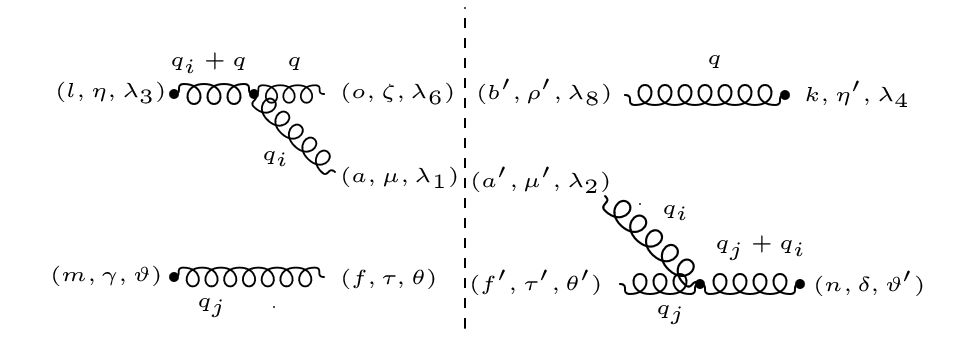
\includegraphics[width=0.95\textwidth]{images/GG/M1DaggerggInverse.png}
\end{figure}

\begin{equation}
\begin{split}
&M_1{M_2}^{\dagger}=[\frac{-i}{(q_i +q)^2}(-g_s f^{\:l\:a\:o}(g^{{\eta}{\mu}}(2q_i+q)^{\zeta}+g^{{\mu}{\zeta}}(q -q_i)^{\eta}-g^{{\zeta}{\eta}}(2q +q_i)^{\mu}){\varepsilon^{\lambda_1}}_{\mu} (q_i) {\varepsilon^{\lambda_6}}_{\zeta}(q)]\\
&[{{\varepsilon^{\theta}}_{{\tau}}}^* (q_j)]\\
&[\frac{i}{(q +q_j)^2}(-g_s f^{\:f^{\prime}\:b^{\prime}\:n }(g^{{{\tau}^{\prime}}{{\rho}^{\prime}}}(q_j-q)^{{\delta}}+g^{{{\rho}^{\prime}}{{\delta}}}(2q +q_j)^{{\tau}^{\prime}}-g^{{{\delta}}{{\tau}^{\prime}}}(2q_j+q)^{{\rho}^{\prime}}){{\varepsilon^{{\theta}^{\prime}}}_{{\tau}^{\prime}}}^* (q_j){{\varepsilon^{\lambda_8}}_{{\rho}^{\prime}}}^* (q)]\\
&[{{\varepsilon^{\lambda_2}}_{{\mu}^{\prime}}}^* (q_i)]
\end{split}
\end{equation}


\begin{equation}
\begin{split}
&M_1{M_2}^{\dagger}=\frac{g_s^2 f^{\:l\:a\:o} f^{\:f^{\prime}\: b^{\prime}\:n} \delta^{aa^{\prime}} \delta^{ob^{\prime}} \delta^{ff^{\prime}}}{(q_i +q)^2 (q_j +q)^2}
[{g_{{\mu}}}^{{\eta}^{\prime}} g_{{\tau}{{\tau}^{\prime}}}(g^{{\eta}{\mu}}(2q_i+q)^{\zeta}+g^{{\mu}{\zeta}}(q -q_i)^{\eta}-g^{{\zeta}{\eta}}(2q +q_i)^{\mu})\\
&g_{{{\zeta}}{{\rho}^{\prime}}}(g^{{{\tau}^{\prime}}{{\rho}^{\prime}}}(q_j-q)^{{\delta}}+g^{{{\rho}^{\prime}}{{\delta}}}(2q +q_j)^{{\tau}^{\prime}}-g^{{{\delta}}{{\tau}^{\prime}}}(2q_j+q)^{{\rho}^{\prime}}]
\end{split}
\end{equation}




\section{$|M^{2}|$}































\chapter{Quark gluon quark emission kernel}

\begin{figure}[ht!]
\centering
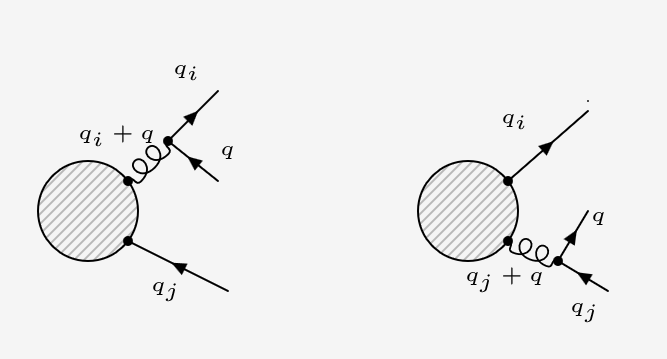
\includegraphics[width=0.85\textwidth]{images/QG/QGDiagrams.png}
\end{figure}

This case concerns a daughter quark from a parent gluon which splits into a quark-anti-quark pair. Here no singularity develops since daughter and parent can always be distinguished.\\
This is the reason why the calculation is not mentioned here, because the evaluation is analogous to the other parts considered so far.
\pagebreak
%
%\section{Quark loop}
%\begin{figure}[ht!]
%\centering
%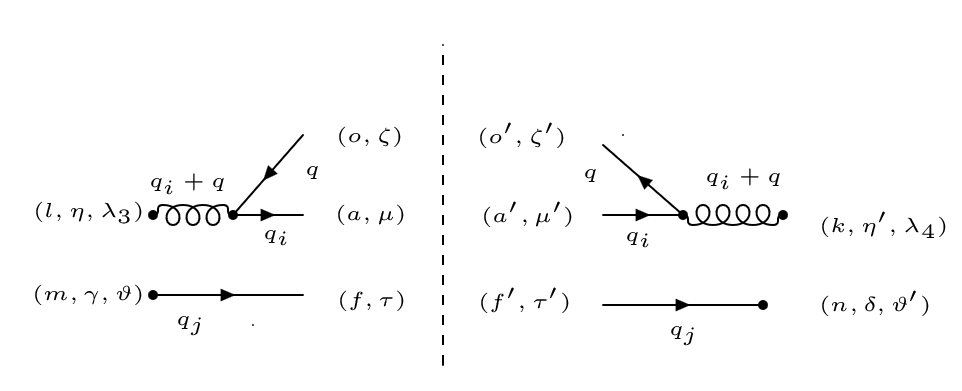
\includegraphics[scale=0.7]{images/QG/M1Squer.png}
%\end{figure}
%
%\begin{equation}
%\begin{split}
%|M_1|^2=[\frac{-i}{(q_i +k_1)^2}\not{q_i}(-ig_s {\gamma}^{\eta}\times{[T^l]_a}^o)\not{q}(ig_s {\gamma}^{{\eta}^{\prime}}\times{[T^k]_{o^{\prime}}}^{a^{\prime}})\frac{i}{(q_i +k_1)^2}][\not{q_k}]
%\end{split}
%\end{equation}
%
%
%\begin{equation}
%\begin{split}
%|M_1|^2=\frac{{g_s}^2 {[T^l]_a}^o {[T^k]_{o^{\prime}}}^{a^{\prime}}}{4(k_1 \cdot q_i)(k_1 \cdot q_i)}[ {k_1}_{\alpha} {q_i}_{\mu}\:(\gamma^{\mu}{\gamma}^{\eta}\gamma^{\alpha}\: {\gamma}^{{\eta}^{\prime}})][\not{q_k}]
%\end{split}
%\end{equation}
%
%
%\begin{equation}
%\begin{split}
%|M_1|^2=\frac{{g_s}^2 {[T^l]_a}^o {[T^k]_{o^{\prime}}}^{a^{\prime}}}{4(k_1 \cdot q_i)(k_1 \cdot q_i)}[{q_i}_{\mu}{k_1}_{\alpha}\:(2g^{{\eta}{\mu}}-{\gamma}^{\eta}\gamma^{\mu})\gamma_{\alpha}\: {\gamma}^{{\eta}^{\prime}}][\not{q_k}]
%\end{split}
%\end{equation}
%
%\begin{equation}
%\begin{split}
%|M_1|^2=\frac{{g_s}^2 {[T^l]_a}^o {[T^k]_{o^{\prime}}}^{a^{\prime}}}{4(k_1 \cdot q_i)(k_1 \cdot q_i)}[(2{q_i}^{\eta}\not{k_1}\:-{\gamma}^{\eta}\not{q_i}\not{k_1})\: {\gamma}^{{\eta}^{\prime}}][\not{q_k}]
%\end{split}
%\end{equation}
%
%\begin{equation}
%\begin{split}
%|M_1|^2=\frac{{g_s}^2 {[T^l]_a}^o {[T^k]_{o^{\prime}}}^{a^{\prime}}}{4(k_1 \cdot q_i)(k_1 \cdot q_i)}[(2{q_i}^{\eta}\not{k_1}\:-{\gamma}^{\eta}\not{q_i}\not{k_1})\: {g}^{{\eta}^{\prime} \eta} \gamma_{\eta}][\not{q_k}]
%\end{split}
%\end{equation}
%
%\begin{equation}
%\begin{split}
%|M_1|^2=\frac{{g_s}^2 {[T^l]_a}^o {[T^k]_{o^{\prime}}}^{a^{\prime}}}{4(k_1 \cdot q_i)(k_1 \cdot q_i)}(2{q_i}^{\eta}\not{k_1}\gamma_{\eta}\:-{\gamma}^{\eta}\not{q_i}\not{k_1}\gamma_{\eta})\: [{g}^{{\eta}^{\prime} \eta} ][\not{q_k}]
%\end{split}
%\end{equation}
%
%\begin{equation}
%\begin{split}
%|M_1|^2=\frac{{g_s}^2 {[T^l]_a}^o {[T^k]_{o^{\prime}}}^{a^{\prime}}}{4(k_1 \cdot q_i)(k_1 \cdot q_i)}(2\not{k_1}\not{q_i}\:-{q_i}_{\mu} {k_1}_{\alpha}{\gamma}^{\eta}{\gamma}^{\mu}{\gamma}^{\alpha}\gamma_{\eta})\: [{g}^{{\eta}^{\prime} \eta} ][\not{q_k}]
%\end{split}
%\end{equation}
%
%\begin{equation}
%\begin{split}
%|M_1|^2=\frac{{g_s}^2 {[T^l]_a}^o {[T^k]_{o^{\prime}}}^{a^{\prime}}}{4(k_1 \cdot q_i)(k_1 \cdot q_i)}(2\not{k_1}\not{q_i}\:-{q_i}_{\mu} {k_1}_{\alpha}(4g^{\alpha \mu}))\: [{g}^{{\eta}^{\prime} \eta} ][\not{q_k}]
%\end{split}
%\end{equation}
%
%\begin{equation}
%\begin{split}
%|M_1|^2=\frac{{g_s}^2 {[T^l]_a}^o {[T^k]_{o^{\prime}}}^{a^{\prime}}}{4(k_1 \cdot q_i)(k_1 \cdot q_i)}(2\not{k_1}\not{q_i}\:-4({q_i} \cdot {k_1}))\: [{g}^{{\eta}^{\prime} \eta} ][\not{q_k}]
%\end{split}
%\end{equation}
%
%\begin{equation}
%\begin{split}
%&|M_1|^2=\frac{{g_s}^2 {[T^l]_a}^o {[T^k]_{o^{\prime}}}^{a^{\prime}}}{4y^2\:(p_i\cdot Q)(p_i\cdot Q) }\\&
%(2(\zeta_1 \not{p_i} + \lambda_1\not{Q} + \sqrt{y\alpha_1\beta_1}\not{n}_{\bot,1} )( \zeta_q\not{p_i} + \lambda_q\not{Q} - \sqrt{y\alpha_1\beta_1}\not{n}_{\bot,l})-4y\:(p_i\cdot Q ))\: [{g}^{{\eta}^{\prime} \eta} ][\not{q_k}]
%\end{split}
%\end{equation}
%
%\begin{equation}
%\begin{split}
%&|M_1|^2=\frac{{g_s}^2 {[T^l]_a}^o {[T^k]_{o^{\prime}}}^{a^{\prime}}}{4y^2\:(p_i\cdot Q)(p_i\cdot Q) }\\&
%(2\zeta_1\lambda_q \not{p_i}\not{Q} +2\lambda_1\zeta_q\not{Q}\not{p_i} - 2{y\alpha_1\beta_1}{{n}_{\bot,1}}^2-4y\:(p_i\cdot Q ))\: [{g}^{{\eta}^{\prime} \eta} ][\not{q_k}]
%\end{split}
%\end{equation}
%
%\begin{equation}
%\begin{split}
%&|M_1|^2=\frac{{g_s}^2 {[T^l]_a}^o {[T^k]_{o^{\prime}}}^{a^{\prime}}}{4y^2\:(p_i\cdot Q)(p_i\cdot Q) }\\&
%(2y\alpha_1^2 \not{p_i}\not{Q} +2y\beta_1^2\not{Q}\not{p_i} - 2{y\alpha_1\beta_1}{{n}_{\bot,1}}^2-4y\:(p_i\cdot Q ))\: [{g}^{{\eta}^{\prime} \eta} ][\not{q_k}]
%\end{split}
%\end{equation}
%
%\pagebreak

%\section{Spectator Quark loop}
%\begin{figure}[ht!]
%\centering
%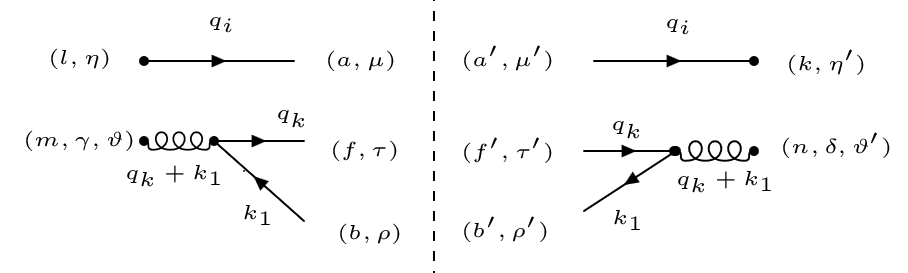
\includegraphics[scale=0.7]{images/QG/M2Squer.png}
%\end{figure}
%
%\begin{equation}
%\begin{split}
%|M_2|^2=\frac{{g_s}^2 {[T^m]_f}^b {[T^n]_{f}}^{b}}{4(k_1 \cdot q_k)(k_1\cdot q_k)}[\not{q_k}{\gamma}^{\gamma}\not{k_1}\:\: {\gamma}^{{\delta}}][\not{q_i}]
%\end{split}
%\end{equation}
%
%\pagebreak
%
%\section{Interference term}
%\begin{figure}[ht!]
%\centering
%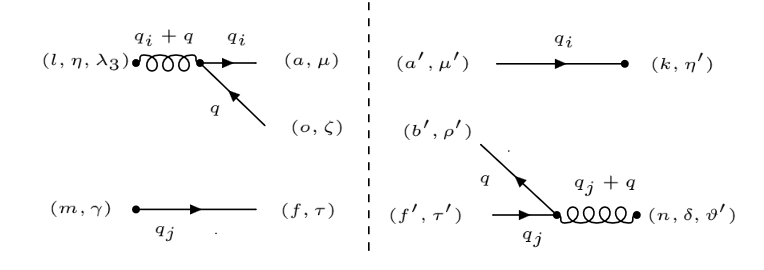
\includegraphics[scale=0.7]{images/QG/M1M2Dagger.png}
%\end{figure}
%
%
%\begin{equation}
%\begin{split}
%M_1\: {M_2}^{\dagger}=\frac{{g_s}^2 {[T^l]_a}^o {[T^n]_{f}}^{o}}{4(k_1 \cdot q_i)(k_1 \cdot q_k)}[\not{q_i}{\gamma}^{\eta}\not{k_1}][\: {\gamma}^{{\delta}}\not{q_k}]
%\end{split}
%\end{equation}
%
%\begin{equation}
%\begin{split}
%M_1\: {M_2}^{\dagger}=\frac{{g_s}^2 {[T^l]_a}^o {[T^n]_{f}}^{o}}{4(k_1\cdot q_i)(k_1 \cdot q_k)}[2\not{q_i}{k_1}^{\eta}-\not{q_i}\not{k_1}{\gamma}^{{\eta}}][\: g^{\delta \eta}{\gamma}_{{\eta}}\not{q_k}]
%\end{split}
%\end{equation}
%
%\begin{equation}
%\begin{split}
%M_1\: {M_2}^{\dagger}=\frac{{g_s}^2 {[T^l]_a}^o {[T^n]_{f}}^{o}}{4(k_1\cdot q_i)(k_1 \cdot q_k)}[2\not{q_i}\not{k_1}-d\not{q_i}\not{k_1}][\: g^{\delta \eta}][\not{q_k}]
%\end{split}
%\end{equation}
%
%\begin{equation}
%\begin{split}
%&M_1\: {M_2}^{\dagger}=(2-d)\frac{{g_s}^2 {[T^l]_a}^o {[T^n]_{f}}^{o}}{4y(1-\beta_1) (1-y)\:(p_i \cdot p_k)(p_i \cdot Q) }\\
%&[((\beta_1 -\alpha_1 y(\frac{Q^2}{2p_i \cdot Q}))\not{p_i} + y\alpha_1\not{Q} - \sqrt{y\alpha_1\beta_1}\not{n}_{\bot,1})\\&((\alpha_1 -y\beta_1(\frac{Q^2}{2p_i \cdot Q})) \not{p_i} + y\beta_1\not{Q} + \sqrt{y\alpha_1\beta_1}\not{n}_{\bot,1})][\: g^{\delta \eta}][\not{q_k}]
%\end{split}
%\end{equation}
%
%\begin{equation}
%\begin{split}
%&M_1\: {M_2}^{\dagger}=(2-d)\frac{{g_s}^2 {[T^l]_a}^o {[T^n]_{f}}^{o}}{4y(1-\beta_1) (1-y)\:(p_i \cdot p_k)(p_i \cdot Q) }\\
%&[\beta_1 \not{p_i}((\alpha_1 -y\beta_1(\frac{Q^2}{2p_i \cdot Q})) \not{p_i} + y\beta_1\not{Q}) ][\: g^{\delta \eta}][\not{q_k}]
%\end{split}
%\end{equation}
%
%\begin{equation}
%\begin{split}
%&M_1\: {M_2}^{\dagger}=(2-d)\frac{{g_s}^2 {[T^l]_a}^o {[T^n]_{f}}^{o}}{4y(1-\beta_1) (1-y)\:(p_i \cdot p_k)(p_i \cdot Q) }[y\beta_1^2 \not{p_i}\not{Q}) ][\: g^{\delta \eta}][\not{q_k}]
%\end{split}
%\end{equation}
%
%\section{$|M^{2}|$}
%
%\begin{equation}
%\begin{split}
%&|M|^{2}=|{M}_2|^{2}+|{M}_1|^{2}+2RE(M_1{M_2}^{\dagger})\\
%\end{split}
%\end{equation}  
\chapter{Gluon quark quark emission kernel}
\section{A daughter gluon from a parent quark}
\begin{figure}[ht!]
\centering
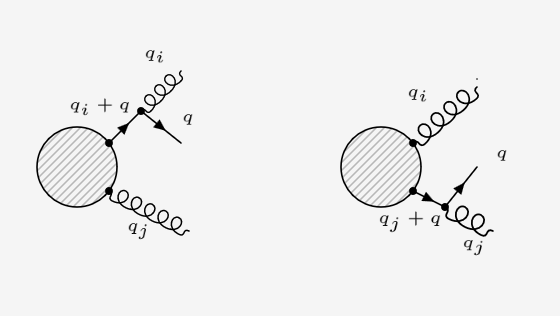
\includegraphics[width=0.85\textwidth]{images/GQ/GQDiagrams.png}
\end{figure}
Since the procedure here is the same as in the previous sections, only the final results are presented here.

\begin{figure}[ht!]
\centering
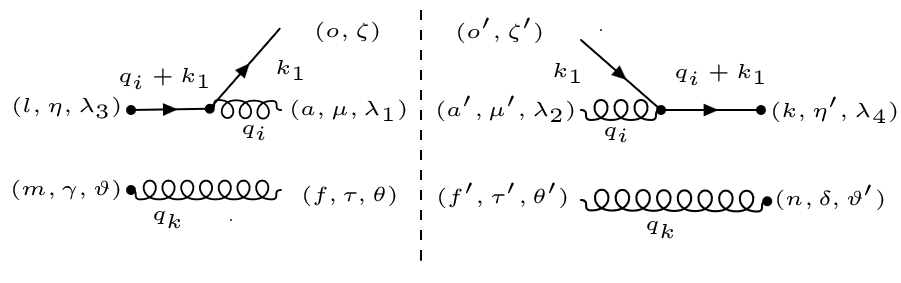
\includegraphics[scale=0.7]{images/GQ/M1Squer.png}
\end{figure}

%\begin{equation}
%\begin{split}
%|M_1|^2=-\frac{{g_s}^2 {[T^{a^{\prime}}]_k}^{o^{\prime}} {[T^a]_{o}}^{l}}{4(k_1 \cdot q_i)(k_1 \cdot q_i)}[(\not{q_i}+\not{k_1}) {\gamma}_{{\mu}}\not{k_1}\:{\gamma}^{\mu}(\not{q_i}+\not{k_1})\:][-{g^{\delta}}_{\gamma}]
%\end{split}
%\end{equation}
%
%\begin{equation}
%\begin{split}
%|M_1|^2=-(2-d)\frac{{g_s}^2 {[T^{a^{\prime}}]_k}^{o^{\prime}} {[T^a]_{o}}^{l}}{4(k_1 \cdot q_i)(k_1 \cdot q_i)}[(\not{q_i}+\not{k_1}) \not{k_1}(\not{q_i}+\not{k_1})\:][-{g^{\delta}}_{\gamma}]
%\end{split}
%\end{equation}
%
%\begin{equation}
%\begin{split}
%|M_1|^2=-(2-d)\frac{{g_s}^2 {[T^{a^{\prime}}]_k}^{o^{\prime}} {[T^a]_{o}}^{l}}{2(k_1 \cdot q_i)}[\not{q_i}][-{g^{\delta}}_{\gamma}]
%\end{split}
%\end{equation}
%
%\begin{equation}
%\begin{split}
%|M_1|^2=-(2-d)\frac{{g_s}^2 C_F}{2y\:p_i \cdot Q}
%[(\alpha_1 -y\beta_1(\frac{Q^2}{2p_i \cdot Q})) \not{p_i} + y\beta_1\not{Q} + \sqrt{y\alpha_1\beta_1}\not{n}_{\bot,1}][-{g^{\delta}}_{\gamma}]
%\end{split}
%\end{equation}

\begin{equation}
\begin{split}
|M_1|^2=(d-2)(1-\beta_1)\frac{{g_s}^2 C_F}{2y \:p_i \cdot Q}
[  \not{p_i}][-{g^{\delta}}_{\gamma}]
\end{split}
\end{equation}


\begin{figure}[ht!]
\centering
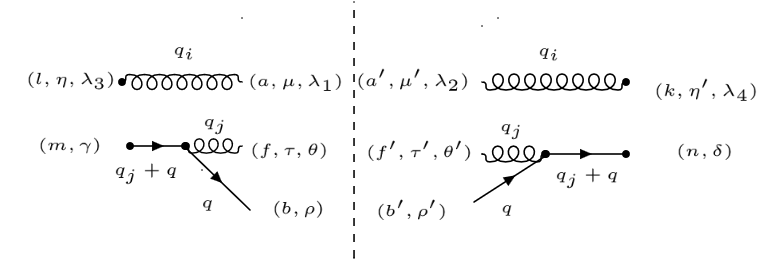
\includegraphics[scale=0.7]{images/GQ/M2Squer.png}
\end{figure}

\begin{equation}
\begin{split}
|M_2|^2=-\frac{{g_s}^2 C_F}{4(k_1 \cdot q_k)(k_1 \cdot q_k)}[(\not{q_k}+\not{k_1}) {\gamma}_{{\tau}^{\prime}}\not{k_1}{\gamma}^{\tau}(\not{q_k}+\not{k_1})][-g^{{\eta}{\eta}^{\prime}}]
\end{split}
\end{equation}

\begin{equation}
\begin{split}
|M_2|^2=(d-2)\frac{{g_s}^2 C_F}{4(k_1 \cdot q_k)}[\not{q_k}][-g^{{\eta}{\eta}^{\prime}}]
\end{split}
\end{equation}



%\begin{figure}[ht!]
%\centering
%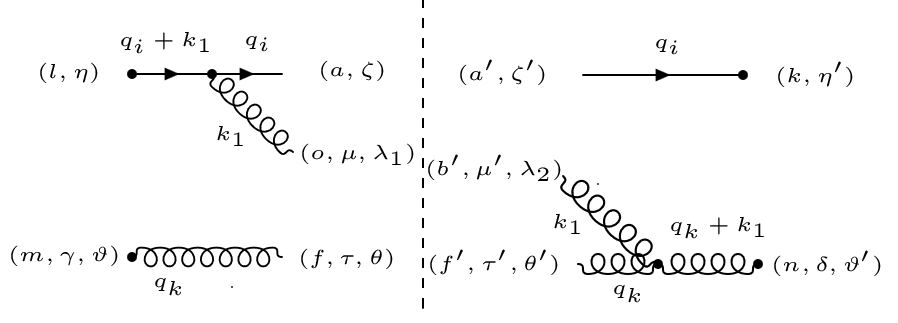
\includegraphics[scale=0.7]{images/GQ/M1M2DaggerGluon.png}
%\end{figure}

%\begin{equation}
%\begin{split}
%&M1{M_2}^{\dagger}=\frac{-{g_s}^2 {[T^{o}]_a}^{l} f^{\:f^{\prime}\: b^{\prime}\:n}}{4(k_1 \cdot q_i)(k_1 \cdot q_k)}[\not{q_i}{\gamma}_{\mu}(\not{k_1}+\not{q_i})\:]\\
%&[ (g^{{{\gamma}}{{\mu}}}(q_k-k_1)^{\delta}+g^{{{\mu}}{{\delta}}}(2k_1 +q_k)^{{\gamma}}-g^{\delta{{\gamma}}}(2q_k+k_1)^{{\mu}})]\\
%\end{split}
%\end{equation}
%
%\begin{equation}
%\begin{split}
%&M1{M_2}^{\dagger}=\frac{-{g_s}^2 {[T^{o}]_a}^{l} f^{\:f^{\prime}\: b^{\prime}\:n}}{4(k_1 \cdot q_i)(k_1 \cdot q_k)}[-\gamma_{\mu}\not{q_i}\not{k_1+2}(\not{k_1}+\not{q_i}){q_i}_{\mu}\:]\\
%&[ g^{{{\gamma}}{{\mu}}}(q_k-k_1)^{\delta}+g^{{{\mu}}{{\delta}}}(2k_1+q_k )^{{\gamma}}-g^{\delta{{\gamma}}}(2q_k+k_1)^{{\mu}}]\\
%\end{split}
%\end{equation}
%
%\begin{equation}
%\begin{split}
%&M1{M_2}^{\dagger}=\frac{-{g_s}^2 {[T^{o}]_a}^{l} f^{\:f^{\prime}\: b^{\prime}\:n}}{4 y(1-\beta_1) (1-y)\:(p_i \cdot p_k)(p_i \cdot Q)}\\
%&[-\gamma_{\mu}((\beta_1 -\alpha_1 y(\frac{Q^2}{2p_i \cdot Q}))\not{p_i} + y\alpha_1\not{Q})((\alpha_1 -y\beta_1(\frac{Q^2}{2p_i \cdot Q})) \not{p_i} + y\beta_1\not{Q})\\
%&+(2((\alpha_1 -y\beta_1(\frac{Q^2}{2p_i \cdot Q})) \not{p_i} + 2y\beta_1\not{Q}+2(\beta_1 -\alpha_1 y(\frac{Q^2}{2p_i \cdot Q}))\not{p_i} + 2y\alpha_1\not{Q})(\beta_1{q_i}_{\mu})\:]\\
%&[ g^{{{\gamma}}{{\mu}}}(-\alpha_1p_i)^{\delta}+g^{{{\mu}}{{\delta}}}(2\alpha_1p_i )^{{\gamma}}-g^{\delta{{\gamma}}}(\alpha_1p_i+(2-y)Q)^{{\mu}}]\\
%\end{split}
%\end{equation}
%
%\begin{equation}
%\begin{split}
%&M1{M_2}^{\dagger}=\frac{-{g_s}^2 C_F}{4 y(1-\beta_1) (1-y)\:(p_i \cdot p_k)(p_i \cdot Q)}\\
%&[-\gamma_{\mu}(y\beta_1^2)\not{p_i}\not{Q}+2(\not{p_i}+y\not{Q})(\beta_1{p_i}_{\mu})\:]\\
%&[ g^{{{\gamma}}{{\mu}}}(-\alpha_1p_i+\sqrt{1-y} p_k)^{\delta}+g^{{{\mu}}{{\delta}}}(2\alpha_1p_i+ \sqrt{1-y} p_k)^{{\gamma}}-g^{\delta{{\gamma}}}(\alpha_1p_i+2\sqrt{1-y} p_k)^{{\mu}}]\\
%\end{split}
%\end{equation}
%
%\begin{equation}
%\begin{split}
%&M1{M_2}^{\dagger}=\frac{-{g_s}^2 C_F}{4 y(1-\beta_1) (1-y)\:(p_i \cdot p_k)(p_i \cdot Q)}\\
%&[-\gamma_{\mu}(y\beta_1^2)\not{p_i}\not{Q}][ g^{{{\gamma}}{{\mu}}}(-\alpha_1p_i+\sqrt{1-y} p_k)^{\delta}+g^{{{\mu}}{{\delta}}}(2\alpha_1p_i+ \sqrt{1-y} p_k)^{{\gamma}}-g^{\delta{{\gamma}}}(\alpha_1p_i+2\sqrt{1-y} p_k)^{{\mu}}]\\
%&+[2(\not{p_i}+y\not{Q})(\beta_1{p_i}_{\mu})\:][ g^{{{\gamma}}{{\mu}}}(-\alpha_1p_i+\sqrt{1-y} p_k)^{\delta}+g^{{{\mu}}{{\delta}}}(2\alpha_1p_i+ \sqrt{1-y} p_k)^{{\gamma}}-g^{\delta{{\gamma}}}(\alpha_1p_i+2\sqrt{1-y} p_k)^{{\mu}}]\\
%\end{split}
%\end{equation}
%
%\begin{equation}
%\begin{split}
%&M1{M_2}^{\dagger}=\frac{-{g_s}^2 C_F}{4 y(1-\beta_1) (1-y)\:(p_i \cdot p_k)(p_i \cdot Q)}\\
%&[-\gamma_{\mu}(y\beta_1^2)\not{p_i}\not{Q}][ g^{{{\gamma}}{{\mu}}}(-\alpha_1p_i)^{\delta}+g^{{{\mu}}{{\delta}}}(\alpha_1p_i )^{{\gamma}}-g^{\delta{{\gamma}}}((2-y)Q)^{{\mu}}][{g^{\delta}}_{\gamma}]\\
%&+[2\beta_1(\not{p_i}+y\not{Q})\:][{p_i}^{\gamma} (-\alpha_1p_i)^{\delta}+{p_i}^{\delta}(2\alpha_1p_i )^{{\gamma}}-g^{\delta{{\gamma}}}(\alpha_1p_i+(2-y))Q\cdot p_i]\\
%\end{split}
%\end{equation}
%
%\begin{equation}
%\begin{split}
%&M1{M_2}^{\dagger}=\frac{-{g_s}^2 C_F}{4 y(1-\beta_1) (1-y)\:(p_i \cdot p_k)(p_i \cdot Q)}\\
%&[-\gamma_{\mu}(y\beta_1^2)\not{p_i}\not{Q}][-g^{\delta{{\gamma}}}(\alpha_1p_i+2\sqrt{1-y} p_k)^{{\mu}}]\\
%&+[2\beta_1(\not{p_i}+y\not{Q})\:][-g^{\delta{{\gamma}}}(\alpha_1p_i+2\sqrt{1-y})p_i\cdot p_k]\\
%\end{split}
%\end{equation}
%
%\begin{equation}
%\begin{split}
%&M1{M_2}^{\dagger}=\frac{-{g_s}^2 C_F}{4 y(1-\beta_1) (1-y)\:(p_i \cdot p_k)(p_i \cdot Q)}\\
%&[-2y\beta_1^2\sqrt{1-y} \not{p_k}\not{p_i}\not{Q}+4\sqrt{1-y}\beta_1(\not{p_i}+y\not{Q})p_i\cdot p_k][-g^{\delta{{\gamma}}}]\\
%\end{split}
%\end{equation}

%\begin{equation}
%\begin{split}
%&M1{M_2}^{\dagger}=\frac{-{g_s}^2 C_F}{y(1-\beta_1) (1-y)\:(p_i \cdot Q)}\sqrt{1-y}\beta_1[\not{p_i}][-g^{\delta{{\gamma}}}]\\
%\end{split}
%\end{equation}

\subsection{Interpretation of the result}

\begin{equation}
\begin{split}
&|M|^{2}=\frac{-{g_s}^2 C_F}{2y (1-y)\:(p_i \cdot Q)}[\not{p_i}][-g^{\delta{{\gamma}}}]\otimes [2RE(\frac{2\beta_1}{1-\beta_1})+(d-2)(1-\beta_1)]\\
\end{split}
\end{equation}

















   
\newpage


\newpage

%\listoftables
%\listoffigures
%\printindex

\chapter*{Appendix A}
\begin{LARGE}
\textbf{MATHEMATICAL TOOLS}
\end{LARGE}
\\
\\

\section*{Lorenz transformation of momenta $ {\hat{{p_i}}}^{\mu}, {\hat{{p_k}}}^{\mu} $ and $ {\hat{{Q}}}^{\mu} $}
\begin{equation*}
\begin{split}
&{\hat{{p_i}}}^{\mu}=\alpha{\Lambda^{\mu}}_{\nu} {p_i}^{\nu}= {p_i}^{\mu} p_{i\nu}{p_i}^{\nu} \frac{-y^2 Q^2}{4(p_i\cdot Q)^2(1+\sqrt{1-y}-\frac{y}{2})}
	+{p_i}^{\mu} Q_{\nu}{p_i}^{\nu} \frac{y(1+\sqrt{1-y})}{2(p_i\cdot Q)(1+\sqrt{1-y}-\frac{y}{2})}\\
&+{Q}^{\mu} p_{i\nu}{p_i}^{\nu} \frac{(y^2 -y-y\sqrt{1-y})}{2(p_i\cdot Q)(1+\sqrt{1-y}-\frac{y}{2})}+\sqrt{1-y} {\eta^{\mu}}_{\nu}{p_i}^{\nu}\\
\end{split}
\end{equation*}

\begin{equation*}
\begin{split}
&{\hat{{p_i}}}^{\mu}={p_i}^{\mu} (Q\cdot p_i) \frac{y(1+\sqrt{1-y})}{2(p_i\cdot Q)(1+\sqrt{1-y}-\frac{y}{2})}+\sqrt{1-y} {p_i}^{\mu}\\
&={p_i}^{\mu} [ \frac{y(1+\sqrt{1-y})}{(2+2\sqrt{1-y}-y)}+\sqrt{1-y}]={p_i}^{\mu}
    \end{split}
\end{equation*}

\begin{equation}
	\begin{aligned}
		\fbox{$  {\hat{{p_i}}}^{\mu}=\alpha{\Lambda^{\mu}}_{\nu} {p_i}^{\nu}= {p_i}^{\mu}$}
    \end{aligned}
\end{equation}


\begin{equation*}
	\begin{aligned}
	{\hat{{p_k}}}^{\mu}=\alpha{\Lambda^{\mu}}_{\nu} {p_k}^{\nu}= {p_i}^{\mu}[  \frac{-y^2 Q^2 (p_{i}\cdot {p_k})}{4(p_i\cdot Q)^2(1+\sqrt{1-y}-\frac{y}{2})}+ \frac{y(1+\sqrt{1-y})(Q \cdot {p_k})}{2(p_i\cdot Q)(1+\sqrt{1-y}-\frac{y}{2})}]\\
	+{Q}^{\mu} [ \frac{(y^2 -y-y\sqrt{1-y}) (p_{i}\cdot {p_k})}{2(p_i\cdot Q)(1+\sqrt{1-y}-\frac{y}{2})}]
	+\sqrt{1-y} {p_k}^{\mu}\\
    \end{aligned}
\end{equation*}


\begin{equation*}
	\begin{aligned}
	{\hat{{p_k}}}^{\mu}&=\alpha{\Lambda^{\mu}}_{\nu} {p_k}^{\nu}= {p_i}^{\mu}[  \frac{-y^2 Q^2 (p_{i}\cdot {p_k})}{4(p_i\cdot Q)^2(1+\sqrt{1-y}-\frac{y}{2})}+ \frac{y(1+\sqrt{1-y})(Q \cdot {p_k})}{2(p_i\cdot Q)(1+\sqrt{1-y}-\frac{y}{2})}]\\
	&+{Q}^{\mu} [ \frac{(y^2 -y-y\sqrt{1-y}) (p_{i}\cdot {p_k})}{2(p_i\cdot Q)(1+\sqrt{1-y}-\frac{y}{2})}]+\sqrt{1-y} {p_k}^{\mu}\\	
\text{with}\\
	A_1 &\equiv  \frac{-y^2 Q^2 (p_{i}\cdot {p_k})}{4(p_i\cdot Q)^2(1+\sqrt{1-y}-\frac{y}{2})}+ \frac{y(1+\sqrt{1-y})(Q \cdot {p_k})}{2(p_i\cdot Q)(1+\sqrt{1-y}-\frac{y}{2})}\\
		A_2 &\equiv   \frac{(y^2 -y-y\sqrt{1-y}) (p_{i}\cdot {p_k})}{2(p_i\cdot Q)(1+\sqrt{1-y}-\frac{y}{2})}\:\:\:\:\:\:\:\:\:\:\:\:\:\:\:\:\:\:\:\:\:\:\:\:\:\:\:\:\:\:\:\:\:\:\:\:\:\:\:\:\:\:\:\:\:\:\:\:\:\:\:\:\:\:\\\
    \end{aligned}    
\end{equation*}

\begin{equation}
	\begin{aligned}
		\fbox{$  {\hat{{p_k}}}^{\mu}= A_1 \:{p_i}^{\mu}+A_2\:{Q}^{\mu}+\sqrt{1-y} {p_k}^{\mu} $}
    \end{aligned}
\end{equation}

\begin{equation*}
	\begin{aligned}
	{\hat{{Q}}}^{\mu}&=\alpha{\Lambda^{\mu}}_{\nu} {Q}^{\nu}= {p_i}^{\mu}[  \frac{-y^2 Q^2 (p_{i}\cdot {Q})}{4(p_i\cdot Q)^2(1+\sqrt{1-y}-\frac{y}{2})}+ \frac{y(1+\sqrt{1-y})Q^2}{2(p_i\cdot Q)(1+\sqrt{1-y}-\frac{y}{2})}]\\
	&+{Q}^{\mu} [ \frac{(y^2 -y-y\sqrt{1-y}) (p_{i}\cdot {Q})}{2(p_i\cdot Q)(1+\sqrt{1-y}-\frac{y}{2})}]
	+\sqrt{1-y} {Q}^{\mu}\\
\text{with}\\
	S_1 &\equiv  \frac{Q^2}{2p_i \cdot Q}[\frac{-y^2}{2(1+\sqrt{1-y}-\frac{y}{2})}+ \frac{y(1+\sqrt{1-y})}{(1+\sqrt{1-y}-\frac{y}{2})}]=\frac{Q^2}{2p_i \cdot Q}y\\
		S_2 &\equiv   \frac{(y^2 -y-y\sqrt{1-y})}{2(1+\sqrt{1-y}-\frac{y}{2})}+\sqrt{1-y}=1-y\:\:\:\:\:\:\:\:\:\:\:\:\:\:\:\:\:\:\:\:\:\:\:\:\:\:\:\:\:\:\:\:\:\:\:\:\:\:\:\:\:\:\:\:\:\:\:\:\:\:\:\:\:\:\\\	
    \end{aligned}    
\end{equation*}

\begin{equation}
	\begin{aligned}
		\fbox{$  {\hat{{Q}}}^{\mu}= \frac{Q^2}{2p_i \cdot Q}y \:{p_i}^{\mu}+(1-y)\:{Q}^{\mu} $}
    \end{aligned}
\end{equation}

\section*{The often occurring pre-factor products}

\begin{equation}
	\begin{split}
	&\zeta_1\zeta_1=({\alpha_1}^2 -2y\alpha_1 \beta_1(\frac{Q^2}{2p_i \cdot Q})+y^2{\beta_1}^2(\frac{Q^2}{2p_i \cdot Q})^2)\\
	&\zeta_1\lambda_1=(y\alpha_1\beta_1 -{y^2\beta_1}^2(\frac{Q^2}{2p_i \cdot Q}))\\
	&\zeta_1\zeta_q=(\alpha_1\beta_1-y({\alpha_1}^2+{\beta_1}^2) (\frac{Q^2}{2p_i \cdot Q})+y^2{\alpha_1}{\beta_1}(\frac{Q^2}{2p_i \cdot Q})^2)\\
	&\zeta_1\lambda_q=(y{\alpha_1}^2 -y^2\beta_1\alpha_1(\frac{Q^2}{2p_i \cdot Q}))\\
	&\zeta_q\zeta_q=	({\beta_1}^2 -2y\alpha_1\beta_1 (\frac{Q^2}{2p_i \cdot Q})+ y^2{\alpha_1}^2 (\frac{Q^2}{2p_i \cdot Q})^2) \\
	&\zeta_q\lambda_1=(y{\beta_1}^2 -y^2\alpha_1 \beta_1(\frac{Q^2}{2p_i \cdot Q}))\\
	&\zeta_q\lambda_q=(y\beta_1\alpha_1 -y^2{\alpha_1}^2(\frac{Q^2}{2p_i \cdot Q}))\\
	&\lambda_1\lambda_1=y^2{\beta_1}^2 \:\:\:\:\:\:\:
	\lambda_1\lambda_q=y^2\beta_1\alpha_1\:\:\:\:\:\:\:\:
	\lambda_q\lambda_q=y^2{\alpha_1}^2\\
    \end{split}
\end{equation}

\section*{Common scalar products}

\begin{equation}
	\begin{aligned}	
k_1 \cdot q_i &= (\zeta_1 \lambda_q + \lambda_1 \zeta_q)p_i \cdot Q+\lambda_1 \lambda_q Q^2 -y\alpha_1\beta_1 {n^{2}}_{\bot,1}\\
	&=[(\alpha_1 -y\beta_1(\frac{Q^2}{2p_i \cdot Q}))y\alpha_1+y\beta_1(\beta_1 -\alpha_1 y(\frac{Q^2}{2p_i \cdot Q}))]\:p_i \cdot Q\\
	&\:\:\:\:\:\:\:y^2\beta_1\alpha_1\: Q^2+2y\alpha_1\beta_1\:p_iQ\\
\Rightarrow	k_1 \cdot q_i &=[y{\alpha_1}^2 -y^2\alpha_1\beta_1(\frac{Q^2}{2p_i \cdot Q})+y {\beta_1}^2-y^2\alpha_1\beta_1(\frac{Q^2}{2p_i \cdot Q})]\:p_i\cdot Q\\
	&y^2\beta_1\alpha_1\: Q^2+2y\alpha_1\beta_1\:p_iQ\\	
    \end{aligned}
\end{equation}

\begin{equation}
	\begin{aligned}
		\fbox{$  k_1 \cdot q_i=y({\alpha_1}+\beta_1)^2\:p_i\cdot Q = y\:p_i\cdot Q $}
    \end{aligned}
\end{equation}

\begin{equation}
	\begin{aligned}	
	k_1 \cdot q_k &= (\zeta_1 A_2 + \lambda_1 A_1)p_i \cdot Q+\zeta_1 \sqrt{1-y}\:p_i\cdot p_k + \lambda_1 A_2\:Q^2+ \lambda_1\sqrt{1-y}\:Q\cdot p_k\\
	&+\sqrt{\alpha_1\beta_1y(1-y)} p_k \cdot {n_{\bot,1}}\\	
	&=\lbrace[(\alpha_1 -y\beta_1(\frac{Q^2}{2p_i \cdot Q}))\frac{(y^2 -y-y\sqrt{1-y}) (p_{i}\cdot {p_k})}{2(p_i\cdot Q)(1+\sqrt{1-y}-\frac{y}{2})}]\\&
	+y\beta_1[\frac{-y^2 Q^2 (p_{i}\cdot {p_k})}{4(p_i\cdot Q)^2(1+\sqrt{1-y}-\frac{y}{2})}+ \frac{y(1+\sqrt{1-y})(Q \cdot {p_k})}{2(p_i\cdot Q)(1+\sqrt{1-y}-\frac{y}{2})}]\rbrace\:p_i \cdot Q\\
	&+(\alpha_1 -y\beta_1(\frac{Q^2}{2p_i \cdot Q}))\sqrt{1-y}\:p_i \cdot p_k+y\beta_1\frac{(y^2 -y-y\sqrt{1-y}) (p_{i}\cdot {p_k})}{2(p_i\cdot Q)(1+\sqrt{1-y}-\frac{y}{2})}Q^2\\
	&+y\beta_1\sqrt{1-y} Q\cdot p_k+\sqrt{\alpha_1\beta_1y(1-y)} p_k \cdot {n_{\bot,1}} 
    \end{aligned}
\end{equation}

\begin{equation}
	\begin{aligned}
	k_1 \cdot q_k &= \alpha_1 \frac{(y^2 -y-y\sqrt{1-y}) }{2(1+\sqrt{1-y}-\frac{y}{2})}(p_{i}\cdot {p_k})
	-y\beta_1(\frac{Q^2}{2p_i \cdot Q})\frac{(y^2 -y-y\sqrt{1-y})}{2(1+\sqrt{1-y}-\frac{y}{2})}(p_{i}\cdot {p_k})\\
&+y\beta_1\frac{-y^2 Q^2 }{4(p_i\cdot Q)(1+\sqrt{1-y}-\frac{y}{2})}(p_{i}\cdot {p_k})+ y\beta_1\frac{y(1+\sqrt{1-y})}{2(1+\sqrt{1-y}-\frac{y}{2})}\:Q \cdot p_k\\
	&+\alpha_1 \sqrt{1-y}\:p_i \cdot p_k-y\beta_1(\frac{Q^2}{2p_i \cdot Q})\sqrt{1-y}\:p_i \cdot p_k\\
	&+y\beta_1(\frac{Q^2}{2p_i \cdot Q})\frac{(y^2 -y-y\sqrt{1-y})}{2(1+\sqrt{1-y}-\frac{y}{2})}(p_{i}\cdot {p_k})+y\beta_1\sqrt{1-y}(Q\cdot p_k)\\
	&+\sqrt{\alpha_1\beta_1y(1-y)} p_k \cdot {n_{\bot,1}} 
    \end{aligned}
\end{equation}

\begin{equation}
	\begin{aligned}
	k_1 \cdot q_k &= [\alpha_1 \frac{(y^2 -y-y\sqrt{1-y}) }{2(1+\sqrt{1-y}-\frac{y}{2})}+y\beta_1\frac{-y^2 Q^2 }{4(p_i\cdot Q)(1+\sqrt{1-y}-\frac{y}{2})}+\alpha_1 \sqrt{1-y}\\&-y\beta_1(\frac{Q^2}{2p_i \cdot Q})\sqrt{1-y}]\:p_i \cdot p_k+[y\beta_1\frac{y(1+\sqrt{1-y})}{2(1+\sqrt{1-y}-\frac{y}{2})}+y\beta_1\sqrt{1-y}](Q\cdot p_k)\\
	&+\sqrt{\alpha_1\beta_1y(1-y)} p_k \cdot {n_{\bot,1}} 
    \end{aligned}
\end{equation}

\begin{equation}
	\begin{aligned}
	k_1 \cdot q_k &= \lbrace\alpha_1 [\frac{(y^2 -y-y\sqrt{1-y}) }{2(1+\sqrt{1-y}-\frac{y}{2})}+ \sqrt{1-y}]\\
	&+y\beta_1(\frac{Q^2}{p_i \cdot Q})[\frac{-y^2 }{4(1+\sqrt{1-y}-\frac{y}{2})}-\sqrt{1-y}]\rbrace\:p_i \cdot p_k\\
	&+y\beta_1[\frac{y(1+\sqrt{1-y})}{2(1+\sqrt{1-y}-\frac{y}{2})}+\sqrt{1-y}](Q\cdot p_k)\\
	&+\sqrt{\alpha_1\beta_1y(1-y)} p_k \cdot {n_{\bot,1}} 
    \end{aligned}
\end{equation}

\begin{equation}
	\begin{aligned}
		\fbox{$  k_1 \cdot q_k = [\alpha_1 (1-y)+y\beta_1(\frac{Q^2}{2p_i \cdot Q})]\:p_i \cdot p_k+y\beta_1\:Q\cdot p_k+\sqrt{\alpha_1\beta_1y(1-y)} p_k \cdot {n_{\bot,1}} $}
    \end{aligned}
\end{equation}

\begin{equation}
	\begin{aligned}	
	q_i \cdot q_k &= (\zeta_q A_2 + \lambda_q A_1)p_i \cdot Q+\zeta_q \sqrt{1-y}\:p_i\cdot p_k + \lambda_q A_2\:Q^2+ \lambda_q\sqrt{1-y}\:Q\cdot p_k\\
	&-\sqrt{\alpha_1\beta_1y(1-y)} p_k \cdot {n_{\bot,1}}\\	
	&=\lbrace[(\beta_1 -y\alpha_1(\frac{Q^2}{2p_i \cdot Q}))\frac{(y^2 -y-y\sqrt{1-y}) (p_{i}\cdot {p_k})}{2(p_i\cdot Q)(1+\sqrt{1-y}-\frac{y}{2})}]\\&
	+y\alpha_1[\frac{-y^2 Q^2 (p_{i}\cdot {p_k})}{4(p_i\cdot Q)^2(1+\sqrt{1-y}-\frac{y}{2})}+ \frac{y(1+\sqrt{1-y})(Q \cdot {p_k})}{2(p_i\cdot Q)(1+\sqrt{1-y}-\frac{y}{2})}]\rbrace\:p_i \cdot Q\\
	&+(\beta_1 -y\alpha_1(\frac{Q^2}{2p_i \cdot Q}))\sqrt{1-y}\:p_i \cdot p_k+y\alpha_1\frac{(y^2 -y-y\sqrt{1-y}) (p_{i}\cdot {p_k})}{2(p_i\cdot Q)(1+\sqrt{1-y}-\frac{y}{2})}Q^2\\
	&+y\alpha_1\sqrt{1-y} Q\cdot p_k-\sqrt{\alpha_1\beta_1y(1-y)} p_k \cdot {n_{\bot,1}} 
    \end{aligned}
\end{equation}


\begin{equation}
	\begin{aligned}
	q_i \cdot q_k &= \beta_1 \frac{(y^2 -y-y\sqrt{1-y}) }{2(1+\sqrt{1-y}-\frac{y}{2})}(p_{i}\cdot {p_k})
	-y\alpha_1(\frac{Q^2}{2p_i \cdot Q})\frac{(y^2 -y-y\sqrt{1-y})}{2(1+\sqrt{1-y}-\frac{y}{2})}(p_{i}\cdot {p_k})\\
&+y\alpha_1\frac{-y^2 Q^2 }{4(p_i\cdot Q)(1+\sqrt{1-y}-\frac{y}{2})}(p_{i}\cdot {p_k})+ y\alpha_1\frac{y(1+\sqrt{1-y})}{2(1+\sqrt{1-y}-\frac{y}{2})}\:Q \cdot p_k\\
	&+\beta_1 \sqrt{1-y}\:p_i \cdot p_k-y\alpha_1(\frac{Q^2}{2p_i \cdot Q})\sqrt{1-y}\:p_i \cdot p_k\\
	&+y\alpha_1(\frac{Q^2}{2p_i \cdot Q})\frac{(y^2 -y-y\sqrt{1-y})}{2(1+\sqrt{1-y}-\frac{y}{2})}(p_{i}\cdot {p_k})+y\alpha_1\sqrt{1-y}(Q\cdot p_k)\\
	&-\sqrt{\alpha_1\beta_1y(1-y)} p_k \cdot {n_{\bot,1}} 
    \end{aligned}
\end{equation}

\begin{equation}
	\begin{aligned}
	q_i \cdot q_k &= [\beta_1 \frac{(y^2 -y-y\sqrt{1-y}) }{2(1+\sqrt{1-y}-\frac{y}{2})}+y\alpha_1\frac{-y^2 Q^2 }{4(p_i\cdot Q)(1+\sqrt{1-y}-\frac{y}{2})}+\beta_1 \sqrt{1-y}\\&-y\alpha_1(\frac{Q^2}{2p_i \cdot Q})\sqrt{1-y}]\:p_i \cdot p_k+[y\alpha_1\frac{y(1+\sqrt{1-y})}{2(1+\sqrt{1-y}-\frac{y}{2})}+y\alpha_1\sqrt{1-y}](Q\cdot p_k)\\
	&-\sqrt{\alpha_1\beta_1y(1-y)} p_k \cdot {n_{\bot,1}} 
    \end{aligned}
\end{equation}

\begin{equation}
	\begin{aligned}
	k_1 \cdot q_k &= \lbrace\beta_1 [\frac{(y^2 -y-y\sqrt{1-y}) }{2(1+\sqrt{1-y}-\frac{y}{2})}+ \sqrt{1-y}]\\
	&+y\alpha_1(\frac{Q^2}{p_i \cdot Q})[\frac{-y^2 }{4(1+\sqrt{1-y}-\frac{y}{2})}-\sqrt{1-y}]\rbrace\:p_i \cdot p_k\\
	&+y\alpha_1[\frac{y(1+\sqrt{1-y})}{2(1+\sqrt{1-y}-\frac{y}{2})}+\sqrt{1-y}](Q\cdot p_k)\\
	&-\sqrt{\alpha_1\beta_1y(1-y)} p_k \cdot {n_{\bot,1}} 
    \end{aligned}
\end{equation}

\begin{equation}
	\begin{aligned}
		\fbox{$  q_i \cdot q_k = [\beta_1 (1-y)+y\alpha_1(\frac{Q^2}{2p_i \cdot Q})]\:p_i \cdot p_k+y\alpha_1\:Q\cdot p_k-\sqrt{\alpha_1\beta_1y(1-y)} p_k \cdot {n_{\bot,1}} $}
    \end{aligned}
\end{equation}

\pagebreak

\section*{Detailed calculation of the gluon radiation of a quark}
\subsection*{$ |M_1|^2 $}

\begin{equation}
\begin{split}
|M_1|^2=(d-2)\:\frac{g_s^2  C_F }{(2k_1\cdot q_i)}
[\not{k_1} ][\not{q_k}]
\end{split}
\end{equation}

\begin{equation}
\begin{split}
&|M_1|^2=(d-2)\:\frac{g_s^2 \: C_F }{2y\: p_i \cdot Q}
[(\alpha_1 -y\beta_1(\frac{Q^2}{2p_i \cdot Q})) \not{p_i} + y\beta_1\not{Q} + \sqrt{y\alpha_1\beta_1}\not{n}_{\bot,1} ]\\
&[A_1\not{p_i} + A_2\not{Q} + \sqrt{1-y}\not{p_k}]
\end{split}
\end{equation}

\begin{equation}
\begin{split}
&|M_1|^2=(d-2)\:\frac{g_s^2 \: C_F }{2y\: p_i \cdot Q}
[(A_2(\alpha_1 -y\beta_1(\frac{Q^2}{2p_i \cdot Q}))+ A_1y\beta_1) {p_i}\cdot Q\\
&+(\alpha_1 -y\beta_1(\frac{Q^2}{2p_i \cdot Q}))\sqrt{1-y}p_i\cdot p_k+A_2 y\beta_1 Q^2+ \sqrt{1-y}\sqrt{y\alpha_1\beta_1}{n}_{\bot,1}\cdot p_k ]\\
\end{split}
\end{equation}

For the collinearity $ y \rightarrow 0 $ we'll get:

\begin{equation}
\begin{split}
&|M_1|^2=(d-2)\:\frac{g_s^2 \: C_F }{2y\: p_i \cdot Q}
[(A_2(\alpha_1 -y\beta_1(\frac{Q^2}{2p_i \cdot Q}))+ A_1y\beta_1) \not{p_i} \not{Q}\\
&+(\alpha_1 -y\beta_1(\frac{Q^2}{2p_i \cdot Q}))\sqrt{1-y}\not{p_i} \not{p_k}+A_2 y\beta_1 Q^2+ \sqrt{1-y}\sqrt{y\alpha_1\beta_1}\not{n}_{\bot,1} \not{p_k} ]\\
\end{split}
\end{equation}

\begin{equation}
\begin{split}
&|M_1|^2=(d-2)(1-\beta_1)\sqrt{1-y}\:\frac{g_s^2 \: C_F }{2y\: p_i \cdot Q}
[\not{p_i} \not{p_k} ]\\
\end{split}
\end{equation}

\subsection*{$ |M_2|^2 $}

\begin{equation}
\begin{split}
|M_2|^2 =(d-2) \frac{g_s^2 \: {[T^c]_f}^m \: {[T^c]_{f}}^n }{2k_1 \cdot q_k} [\not{k_1}]\: 
[\not{q_i} ]
\end{split}
\end{equation}

\begin{equation}
\begin{split}
&|M_2|^2 =(d-2) \frac{g_s^2 \: C_F}{2k_1 \cdot q_k} [(\alpha_1 -y\beta_1(\frac{Q^2}{2p_i \cdot Q})) \not{p_i} + y\beta_1\not{Q} + \sqrt{y\alpha_1\beta_1}\not{n}_{\bot,1}]\: \\
&[(\beta_1 -\alpha_1 y(\frac{Q^2}{2p_i \cdot Q}))\not{p_i} + y\alpha_1\not{Q} - \sqrt{y\alpha_1\beta_1}\not{n}_{\bot,l} ]
\end{split}
\end{equation}


\begin{equation}
\begin{split}
&|M_2|^2 =(d-2) \frac{g_s^2 \: C_F}{2k_1 \cdot q_k} [y\alpha_1(\alpha_1 -y\beta_1(\frac{Q^2}{2p_i \cdot Q}))\not{p_i}\not{Q}  + y\beta_1(\beta_1 -\alpha_1 y(\frac{Q^2}{2p_i \cdot Q}))]\not{Q}\not{p_i}\\
&+y^2\alpha_1\beta_1 Q^2-y\beta_1\sqrt{y\alpha_1\beta_1}\not{Q}\not{n}_{\bot,1}+y\beta_1\sqrt{y\alpha_1\beta_1}\not{n}_{\bot,1}\not{Q}- y\alpha_1\beta_1 \:{{n}_{\bot,l}}^2 \\
&+ (\beta_1 -\alpha_1 y(\frac{Q^2}{2p_i \cdot Q})\sqrt{y\alpha_1\beta_1}\not{n}_{\bot,1}\not{p_i}- (\alpha_1 -\alpha_1 y(\frac{Q^2}{2p_i \cdot Q})\sqrt{y\alpha_1\beta_1}\not{p_i}\not{n}_{\bot,1} ]
\end{split}
\end{equation}

Which means:
\begin{equation}
\begin{split}
&|M_2|^2 \sim(d-2) \frac{g_s^2 \: C_F}{2k_1 \cdot q_k} y[...]\\
&\:\:\:\:\:\:\:\:|M_2|^2\rightarrow 0 \:\:\:\:\:\:\:\text{for}\:\:\:\:\: y\rightarrow 0
\end{split}
\end{equation}

\subsection*{$ M_1\: {M_2}^{\dagger} $}

\begin{equation}
\begin{split}
&M_1\: {M_2}^{\dagger} = \frac{-g_s^2 {[T^a]_o}^l \:{[T^a]_{f^{\prime}}}^n }{(2q_i k_1)(2q_k k_1)} 
[(\not{q_i} + \not{k_1})\:\not{q_i}\: \gamma^{\mu}] \:[(\not{q_k} + \not{k_1}) \not{q_k} \gamma_{\mu}] \\
&+4[(\not{q_i} + \not{k_1})\:{q_{i}}^{\mu}][(\not{q_k} + \not{k_1}) {q_{k{\mu}}}]
\end{split}
\end{equation}

\begin{equation}
\begin{split}
&M_1\: {M_2}^{\dagger} = \frac{-g_s^2\: C_F }{4y(1-\beta_1) (1-y)\:(p_i \cdot p_k)(p_i \cdot Q)} \\
&[(\not{q_i}\not{q_i} + \not{k_1}\not{q_i})\: \gamma^{\mu}] [(\not{q_k}\not{q_k} + \not{k_1}\not{q_k})  \gamma_{\mu}] +4({{q_{i}}^{\mu}q_{k{\mu}}})[\not{q_i} + \not{k_1}\:][\not{q_k} + \not{k_1} ]
\end{split}
\end{equation}

\begin{equation}
\begin{split}
&M_1\: {M_2}^{\dagger} = \frac{-g_s^2\: C_F }{4y(1-\beta_1) (1-y)\:(p_i \cdot p_k)(p_i \cdot Q)} \\
&[\not{k_1}\not{q_i}\: \gamma^{\mu}] [ \not{k_1}\not{q_k}  \gamma_{\mu}] +4({q_{i}}\cdot q_k)[\not{q_i}\not{q_k} + \not{k_1}\not{q_k}+\not{q_i}\not{k_1} ]
\end{split}
\end{equation}

\begin{equation}
\begin{split}
&M_1\: {M_2}^{\dagger} = \frac{-g_s^2\: C_F }{4y(1-\beta_1) (1-y)\:(p_i \cdot p_k)(p_i \cdot Q)} \\
&4(A_1\beta_1 {p_i}\cdot{p_i}+A_2\beta_1 {p_i}\cdot {{Q}}+\beta_1 \sqrt{1-y}{p_i}\cdot {{p_k}})\\
&[A_1\beta_1 \not{p_i}\not{p_i}+A_2\beta_1 \not{p_i}\not{Q}+\beta_1 \sqrt{1-y}\not{p_i} \not{p_k}\\
&+ [(1-\beta_1)-y\beta_1 (\frac{Q^2}{2p_i \cdot Q})] \sqrt{1-y}\not{p_i}\not{p_k}-y {\beta_1} (\frac{Q^2}{2p_i \cdot Q}) A_1 \:\not{p_i}\not{p_i}\\
&-y {\beta_1} (\frac{Q^2}{2p_i \cdot Q}) A_2\: \not{p_i}\not{Q}+y {\beta_1} A_1 \:\not{Q}\not{p_i}+y {\beta_1} A_2 \:\not{Q}\not{Q}+y {\beta_1}\sqrt{1-y}\not{Q}\not{p_k}\\
&+[\beta_1(1-\beta_1)-y {\beta_1}^2 (\frac{Q^2}{2p_i \cdot Q})] \not{p_i}\not{p_i}+y {\beta_1}^2 \not{p_i}\not{Q} ]
\end{split}
\end{equation}

\begin{equation}
\begin{split}
&M_1\: {M_2}^{\dagger} = \frac{-g_s^2\: C_F }{4y(1-\beta_1) (1-y)\:(p_i \cdot p_k)(p_i \cdot Q)} \\
&4(A_2\beta_1 {p_i}\cdot {{Q}}+\beta_1 \sqrt{1-y}{p_i}\cdot {{p_k}})[A_2\beta_1 \not{p_i}\not{Q}+\beta_1 \sqrt{1-y}\not{p_i} \not{p_k}\\
&+ [(1-\beta_1)-y\beta_1 (\frac{Q^2}{2p_i \cdot Q})] \sqrt{1-y}\not{p_i}\not{p_k}-y {\beta_1} (\frac{Q^2}{2p_i \cdot Q}) A_2\: \not{p_i}\not{Q}\\
&+y {\beta_1} A_1 \:\not{Q}\not{p_i}+y {\beta_1} A_2 \:\not{Q}\not{Q}+y {\beta_1}\sqrt{1-y}\not{Q}\not{p_k}+y {\beta_1}^2 \not{p_i}\not{Q} ]
\end{split}
\end{equation}

\begin{equation}
\begin{split}
&M_1\: {M_2}^{\dagger} = \frac{-g_s^2\: C_F }{4y(1-\beta_1) (1-y)\:(p_i \cdot p_k)(p_i \cdot Q)} \\
&4(\beta_1 \sqrt{1-y}{p_i}\cdot {{p_k}})[\beta_1 \sqrt{1-y}\not{p_i} \not{p_k}+ (1-\beta_1) \sqrt{1-y}\not{p_i}\not{p_k}]
\end{split}
\end{equation}

\begin{equation}
\begin{split}
&M_1\: {M_2}^{\dagger} = \frac{-g_s^2\: C_F }{y(1-\beta_1) \:(p_i \cdot p_k)(p_i \cdot Q)} \beta_1( {p_i}\cdot {{p_k}})[\beta_1 \not{p_i} \not{p_k}+ (1-\beta_1) \not{p_i}\not{p_k}]
\end{split}
\end{equation}

\begin{equation}
\begin{split}
&M_1\: {M_2}^{\dagger} = \frac{\beta_1}{(1-\beta_1)}\: \frac{-g_s^2\: C_F }{y \:(p_i \cdot Q)} [\not{p_i} \not{p_k}]
\end{split}
\end{equation}

\subsection*{Evaluation of the tensor $N^{{\eta}{{\eta}^{\prime}}}$}

\begin{equation}
\begin{split}
N^{{\eta}{{\eta}^{\prime}}}\equiv g_{{\mu}{{\mu}^{\prime}}} g_{{\zeta}{{\zeta}^{\prime}}}[-g^{{\mu}{\zeta}}g^{{{\mu}^{\prime}}{{\eta}^{\prime}}}(q-q_i)^{{\eta}}(2q_i+q)^{{\zeta}^{\prime}}+g^{{\mu}{\zeta}}g^{{{\eta}^{\prime}}{{\zeta}^{\prime}}}(q-q_i)^{\eta}(2q +q_i)^{{\mu}^{\prime}}\\+g^{{\mu}{\zeta}}g^{{{\zeta}^{\prime}}{{\mu}^{\prime}}}(q-q_i)^{\eta}(q_i -q)^{{\eta}^{\prime}}+g^{{\zeta}{\eta}}g^{{{\mu}^{\prime}}{{\zeta}^{\prime}}}(2q +q_i)^{\mu}(2q_i+q)^{{\zeta}^{\prime}}\\
-g^{{\zeta}{\eta}}g^{{{\eta}^{\prime}}{{\zeta}^{\prime}}}(2q +q_i)^{\mu}(2q +q_i)^{{\mu}^{\prime}}-g^{{\zeta}{\eta}}g^{{{\zeta}^{\prime}}{{\mu}^{\prime}}}(2q +q_i)^{\mu}(q_i -q)^{{\eta}^{\prime}}\\
-g^{{\eta}{\mu}}g^{{{\mu}^{\prime}}{{\eta}^{\prime}}}(2q_i +q)^{\zeta}(2q_i+q)^{{\zeta}^{\prime}}+g^{{\eta}{\mu}}g^{{{\eta}^{\prime}}{{\zeta}^{\prime}}}(2q_i +q)^{\zeta}(2q +q_i)^{{\mu}^{\prime}}\\
+g^{{\eta}{\mu}}g^{{{\zeta}^{\prime}}{{\mu}^{\prime}}}(2q_i +q)^{\zeta}(q_i -q)^{{\eta}^{\prime}}][g^{{\gamma}{\delta}}]
\end{split}
\end{equation}


\begin{equation}
\begin{split}
N^{{\eta}{{\eta}^{\prime}}}\equiv [-(q-q_i)^{{\eta}}(2q_i+q)^{{\eta}^{\prime}}+(q-q_i)^{\eta}(2q +q_i)^{{\eta}^{\prime}}+d(q-q_i)^{\eta}(q_i -q)^{{\eta}^{\prime}}\\+(2q +q_i)^{{\eta}^{\prime}}(2q_i+q)^{{\eta}}
-g^{{\eta}{{\eta}^{\prime}}}(2q +q_i)^{\mu}(2q +q_i)_{{\mu}}-(2q +q_i)^{\eta}(q_i -q)^{{\eta}^{\prime}}\\
-g^{{\eta}{{\eta}^{\prime}}}(2q_i +q)^{\zeta}(2q_i+q)_{{\zeta}}+(2q_i +q)^{{\eta}^{\prime}}(2q +q_i)^{{\eta}}
+(2q_i +q)^{\eta}(q_i -q)^{{\eta}^{\prime}}][g^{{\gamma}{\delta}}]
\end{split}
\end{equation}

\begin{equation}
\begin{split}
N^{{\eta}{{\eta}^{\prime}}}\equiv [-({q}^{{\eta}}{q}^{{\eta}^{\prime}}+2{q}^{{\eta}}{q_i}^{{\eta}^{\prime}}-{q_i}^{{\eta}}{q}^{{\eta}^{\prime}}-2{q_i}^{{\eta}}{q_i}^{{\eta}^{\prime}})
+(2{q}^{{\eta}}{q}^{{\eta}^{\prime}}+{q}^{{\eta}}{q_i}^{{\eta}^{\prime}}-2{q_i}^{{\eta}}{q}^{{\eta}^{\prime}}-{q_i}^{{\eta}}{q_i}^{{\eta}^{\prime}})\\+(d{q}^{{\eta}}{q_i}^{{\eta}^{\prime}}-d{q}^{{\eta}}{q}^{{\eta}^{\prime}}-d{q_i}^{{\eta}}{q_i}^{{\eta}^{\prime}}+d{q_i}^{{\eta}}{q}^{{\eta}^{\prime}})+(4{q}^{{\eta}^{\prime}}{q_i}^{{\eta}}+2{q}^{{\eta}^{\prime}}{q}^{{\eta}}+2{q_i}^{{\eta}^{\prime}}{q_i}^{{\eta}}+{q_i}^{{\eta}^{\prime}}{q}^{{\eta}})\\
-(-2{q}^{{\eta}}{q}^{{\eta}^{\prime}}+2{q}^{{\eta}}{q_i}^{{\eta}^{\prime}}-{q_i}^{{\eta}}{q}^{{\eta}^{\prime}}+{q_i}^{{\eta}}{q_i}^{{\eta}^{\prime}})+(2{q}^{{\eta}^{\prime}}{q}^{{\eta}}+{q}^{{\eta}^{\prime}}{q_i}^{{\eta}}+4{q_i}^{{\eta}^{\prime}}{q}^{{\eta}}+2{q_i}^{{\eta}^{\prime}}{q_i}^{{\eta}})\\+(-{q}^{{\eta}}{q}^{{\eta}^{\prime}}+{q}^{{\eta}}{q_i}^{{\eta}^{\prime}}-2{q_i}^{{\eta}}{q}^{{\eta}^{\prime}}+2{q_i}^{{\eta}}{q_i}^{{\eta}^{\prime}})
-g^{{\eta}{{\eta}^{\prime}}}(5{q}^2+5{q_i}^2+8qq_i)][g^{{\gamma}{\delta}}]
\end{split}
\end{equation}

\section{Evaluation of the interference term $M_1 {M_2}^{\dagger}$}
\label{EvaIntGG}

\subsection*{Calculation of the first Term}

\begin{equation}
\begin{split} 
& g^{{{\eta}}{{\eta}^{\prime}}}[2\lbrace A_1\beta_1 {p_i}^{{\gamma}}{{p_i}^{{\delta}}}+A_2\beta_1 {p_i}^{{\gamma}}{{Q}^{{\delta}}}+\beta_1 \sqrt{1-y}{p_i}^{{\gamma}}{{p_k}^{{\delta}}} \rbrace \\&
+2\lbrace [\beta_1(1-\beta_1)-y {\beta_1}^2 (\frac{Q^2}{2p_i \cdot Q})] {p_i}^{{\gamma}}{p_i}^{{\delta}}+y {\beta_1}^2 {p_i}^{{\gamma}}{Q}^{{\delta}} \rbrace\\
&+\lbrace [(1-\beta_1)-y\beta_1 (\frac{Q^2}{2p_i \cdot Q})] \sqrt{1-y}{p_i}^{{\gamma}}{{p_k}^{{\delta}}}-y {\beta_1} (\frac{Q^2}{2p_i \cdot Q}) A_1 \:{p_i}^{{\gamma}}{p_i}^{{\delta}}
-y {\beta_1} (\frac{Q^2}{2p_i \cdot Q}) A_2\: {p_i}^{{\gamma}}{Q}^{{\delta}}\\
&+y {\beta_1} A_1 \:{Q}^{{\gamma}}{p_i}^{{\delta}}+y {\beta_1} A_2 \:{Q}^{{\gamma}}{Q}^{{\delta}}+y {\beta_1}\sqrt{1-y}{Q}^{{\gamma}}{{p_k}^{{\delta}}} \rbrace \\
&+3\lbrace [(1-\beta_1)^2-y^2 {\beta_1}^2 (\frac{Q^2}{2p_i \cdot Q})^2] {p_i}^{{\gamma}}{p_i}^{{\delta}}-y^2 {\beta_1}^2 (\frac{Q^2}{2p_i \cdot Q}){p_i}^{{\gamma}}{Q}^{{\delta}}-y^2 {\beta_1}^2 (\frac{Q^2}{2p_i \cdot Q}){Q}^{{\gamma}}{p_i}^{{\delta}} \rbrace\\
&+4\lbrace [\beta_1(1-\beta_1)-y {\beta_1}^2 (\frac{Q^2}{2p_i \cdot Q})] {p_i}^{{\gamma}}{p_i}^{{\delta}}+y {\beta_1}^2 {Q}^{{\gamma}}{p_i}^{{\delta}} \rbrace\\
&+2\lbrace A_1\beta_1 {p_i}^{{\gamma}}{{p_i}^{{\delta}}}+A_2\beta_1 {Q}^{{\gamma}}{{p_i}^{{\delta}}}+\beta_1 \sqrt{1-y}{p_k}^{{\gamma}}{{p_i}^{{\delta}}} \rbrace \\
&+\lbrace [(1-\beta_1)-y\beta_1 (\frac{Q^2}{2p_i \cdot Q})] \sqrt{1-y}{p_k}^{{\gamma}}{{p_i}^{{\delta}}}-y {\beta_1} (\frac{Q^2}{2p_i \cdot Q}) A_1 \:{p_i}^{{\gamma}}{p_i}^{{\delta}}
-y {\beta_1} (\frac{Q^2}{2p_i \cdot Q}) A_2\: {Q}^{{\gamma}}{p_i}^{{\delta}}\\
&+y {\beta_1} A_1 \:{p_i}^{{\gamma}}{Q}^{{\delta}}+y {\beta_1} A_2 \:{Q}^{{\gamma}}{Q}^{{\delta}}+y {\beta_1}\sqrt{1-y}{p_k}^{{\gamma}}{{Q}^{{\delta}}} \rbrace]\\
\end{split}
\end{equation}

%\begin{equation}
%\begin{split} 
%& g^{{{\eta}}{{\eta}^{\prime}}}\lbrace [2 A_1\beta_1+2 [\beta_1(1-\beta_1)-y {\beta_1}^2 (\frac{Q^2}{2p_i \cdot Q})]\\
%&+4 [\beta_1(1-\beta_1)-y {\beta_1}^2 (\frac{Q^2}{2p_i \cdot Q})]+3 [(1-\beta_1)^2-y^2 {\beta_1}^2 (\frac{Q^2}{2p_i \cdot Q})^2]\\
%&+2 A_1\beta_1 -y {\beta_1} (\frac{Q^2}{2p_i \cdot Q}) A_1\:-y {\beta_1} (\frac{Q^2}{2p_i \cdot Q}) A_1 \:] {p_i}^{{\gamma}}{{p_i}^{{\delta}}}\\
%&+[2A_2\beta_1+2y {\beta_1}^2 -y {\beta_1} (\frac{Q^2}{2p_i \cdot Q}) A_2\: -3y^2 {\beta_1}^2 (\frac{Q^2}{2p_i \cdot Q})+y {\beta_1} A_1] {p_i}^{{\gamma}}{{Q}^{{\delta}}}\\
%&+[2\beta_1+[(1-\beta_1)-y\beta_1 (\frac{Q^2}{2p_i \cdot Q})] ] \sqrt{1-y}{p_i}^{{\gamma}}{{p_k}^{{\delta}}} \\
%&+[y {\beta_1} A_1+4y {\beta_1}^2 +2A_2\beta_1 -3y^2 {\beta_1}^2 (\frac{Q^2}{2p_i \cdot Q})-y {\beta_1} (\frac{Q^2}{2p_i \cdot Q}) A_2\: ] \:{Q}^{{\gamma}}{p_i}^{{\delta}}\\
%&+[y {\beta_1} A_2+y {\beta_1} A_2] \:{Q}^{{\gamma}}{Q}^{{\delta}}+y {\beta_1}\sqrt{1-y}{Q}^{{\gamma}}{{p_k}^{{\delta}}} \\
%&+[2\beta_1 + [(1-\beta_1)-y\beta_1 (\frac{Q^2}{2p_i \cdot Q})] ]\sqrt{1-y}{p_k}^{{\gamma}}{{p_i}^{{\delta}}}+y {\beta_1}\sqrt{1-y}{p_k}^{{\gamma}}{{Q}^{{\delta}}}\rbrace\\
%\end{split}
%\end{equation}

\subsection*{Calculation of the second term}

\begin{equation}
\begin{split}
&{\color[RGB]{255,0,0} -g^{{{\eta}}{{\eta}^{\prime}}}g^{{{\gamma}}{{\delta}}}}( 2q\cdot q_j+ q\cdot q+4q_i \cdot q_j+2q_i \cdot q)
\end{split}
\end{equation}

\begin{equation}
\begin{split}
&{\color[RGB]{255,0,0} -g^{{{\eta}}{{\eta}^{\prime}}}g^{{{\gamma}}{{\delta}}}}[ 2([\alpha_1 (1-y)+y\beta_1(\frac{Q^2}{2p_i \cdot Q})]\:p_i \cdot p_k+y\beta_1\:Q\cdot p_k+\sqrt{\alpha_1\beta_1y(1-y)} p_k \cdot {n_{\bot,1}})\\
&4([\beta_1 (1-y)+y\alpha_1(\frac{Q^2}{2p_i \cdot Q})]\:p_i \cdot p_k+y\alpha_1\:Q\cdot p_k-\sqrt{\alpha_1\beta_1y(1-y)} p_k \cdot {n_{\bot,1}})\\
&+2(y\:p_i\cdot Q)]
\end{split}
\end{equation}




\subsection*{Calculation of the third term}
\begin{equation}
\begin{split} 
&+g^{{{\gamma}}{{\eta}^{\prime}}}\lbrace [(1-\beta_1)-y\beta_1 (\frac{Q^2}{2p_i \cdot Q})] \sqrt{1-y}{p_i}^{{\eta}}{{p_k}^{{\delta}}}-y {\beta_1} (\frac{Q^2}{2p_i \cdot Q}) A_1 \:{p_i}^{{\eta}}{p_i}^{{\delta}}
-y {\beta_1} (\frac{Q^2}{2p_i \cdot Q}) A_2\: {p_i}^{{\eta}}{Q}^{{\eta}^{\prime}}\\
&+y {\beta_1} A_1 \:{Q}^{{\eta}}{p_i}^{{\delta}}+y {\beta_1} A_2 \:{Q}^{{\eta}}{Q}^{{\delta}}+y {\beta_1}\sqrt{1-y}{Q}^{{\eta}}{{p_k}^{{\delta}}}\\
&-[[(1-\beta_1)^2-y^2 {\beta_1}^2 (\frac{Q^2}{2p_i \cdot Q})^2] {p_i}^{{\eta}}{p_i}^{{\delta}}-y^2 {\beta_1}^2 (\frac{Q^2}{2p_i \cdot Q}){p_i}^{{\eta}}{Q}^{{\delta}}-y^2 {\beta_1}^2 (\frac{Q^2}{2p_i \cdot Q}){Q}^{{\eta}}{p_i}^{{\delta}}]\\
&-[A_1\beta_1 {p_i}^{{\eta}}{{p_i}^{{\delta}}}+A_2\beta_1 {p_i}^{{\eta}}{{Q}^{{\delta}}}+\beta_1 \sqrt{1-y}{p_i}^{{\eta}}{{p_k}^{{\delta}}}]\\
&+[\beta_1(1-\beta_1)-y {\beta_1}^2 (\frac{Q^2}{2p_i \cdot Q})] {p_i}^{{\eta}}{p_i}^{{\eta}^{\prime}}+y {\beta_1}^2 {p_i}^{{\eta}}{Q}^{{\eta}^{\prime}}\rbrace\\
\end{split}
\end{equation}

\subsection*{Calculation of the fourth term}

\begin{equation}
\begin{split} 
&+g^{{{\eta}^{\prime}}{{\delta}}}\lbrace [(1-\beta_1)-y\beta_1 (\frac{Q^2}{2p_i \cdot Q})-\beta_1] \sqrt{1-y}{p_i}^{{\eta}}{{p_k}^{{\gamma}}}\\
&+[2[(1-\beta_1)^2-y^2 {\beta_1}^2 (\frac{Q^2}{2p_i \cdot Q})^2]-y {\beta_1} (\frac{Q^2}{2p_i \cdot Q}) A_1 +A_1\beta_1 +\\
&[\beta_1(1-\beta_1)-y {\beta_1}^2 (\frac{Q^2}{2p_i \cdot Q})]] {p_i}^{{\eta}}{p_i}^{{\gamma}}\\
& +[-2y^2 {\beta_1}^2 (\frac{Q^2}{2p_i \cdot Q})-y {\beta_1} (\frac{Q^2}{2p_i \cdot Q}) A_2\:+A_2\beta_1 +y {\beta_1}^2] {p_i}^{{\eta}}{Q}^{{\gamma}}\\
&+[y {\beta_1} A_1 \:+2y^2 {\beta_1}^2 (\frac{Q^2}{2p_i \cdot Q})]{Q}^{{\eta}}{p_i}^{{\gamma}}+y {\beta_1} A_2 \:{Q}^{{\eta}}{Q}^{{\gamma}}+y {\beta_1}\sqrt{1-y}{Q}^{{\eta}}{{p_k}^{{\gamma}}}
\rbrace\\
\end{split}
\end{equation}

\subsection*{Calculation of the fifth term}

\begin{equation}
\begin{split} 
&-g^{{{\gamma}}{{\delta}}}\lbrace[2[(1-\beta_1)-y\beta_1 (\frac{Q^2}{2p_i \cdot Q})]-2\beta_1] \sqrt{1-y}{p_i}^{{\eta}}{{p_k}^{{\eta}^{\prime}}}\\
&[-2y {\beta_1} (\frac{Q^2}{2p_i \cdot Q}) A_1+[(1-\beta_1)^2-y^2 {\beta_1}^2 (\frac{Q^2}{2p_i \cdot Q})^2]-2A_1\beta_1\\
&-[\beta_1(1-\beta_1)-y {\beta_1}^2 (\frac{Q^2}{2p_i \cdot Q})] ]\:{p_i}^{{\eta}}{p_i}^{{\eta}^{\prime}}\\
&[-2y {\beta_1} (\frac{Q^2}{2p_i \cdot Q}) A_2\: -y^2 {\beta_1}^2 (\frac{Q^2}{2p_i \cdot Q})-y {\beta_1}^2 -2A_2\beta_1 ]{p_i}^{{\eta}}{Q}^{{\eta}^{\prime}}\\
&+[2y {\beta_1} A_1-y^2 {\beta_1}^2 (\frac{Q^2}{2p_i \cdot Q})] \:{Q}^{{\eta}}{p_i}^{{\eta}^{\prime}}+2y {\beta_1} A_2 \:{Q}^{{\eta}}{Q}^{{\eta}^{\prime}}+2y {\beta_1}\sqrt{1-y}{Q}^{{\eta}}{{p_k}^{{\eta}^{\prime}}}\rbrace\\
\end{split}
\end{equation}

\subsection*{Calculation of the sixth term}
\begin{equation}
\begin{split}
&-g^{{{\gamma}}{{\eta}}}\lbrace[2[(1-\beta_1)-y\beta_1 (\frac{Q^2}{2p_i \cdot Q})]+\beta_1 ] \sqrt{1-y}{p_i}^{{\eta}^{\prime}}{{p_k}^{{\delta}}}\\
&[-2y {\beta_1} (\frac{Q^2}{2p_i \cdot Q}) A_1-2[(1-\beta_1)^2-y^2 {\beta_1}^2 (\frac{Q^2}{2p_i \cdot Q})^2]\\
&-[\beta_1(1-\beta_1)-y {\beta_1}^2 (\frac{Q^2}{2p_i \cdot Q})] +A_1\beta_1 ] \:{p_i}^{{\eta}^{\prime}}{p_i}^{{\delta}}\\
&[-2y {\beta_1} (\frac{Q^2}{2p_i \cdot Q}) A_2\:+2y^2 {\beta_1}^2 (\frac{Q^2}{2p_i \cdot Q})+A_2\beta_1 -y {\beta_1}^2 ] {p_i}^{{\eta}^{\prime}}{Q}^{{\delta}}\\
&+[2y {\beta_1} A_1+2y^2 {\beta_1}^2 (\frac{Q^2}{2p_i \cdot Q})] \:{Q}^{{\eta}^{\prime}}{p_i}^{{\delta}}+2y {\beta_1} A_2 \:{Q}^{{\eta}^{\prime}}{Q}^{{\delta}}+2y {\beta_1}\sqrt{1-y}{Q}^{{\eta}^{\prime}}{{p_k}^{{\delta}}}
\rbrace
\end{split}
\end{equation}

\subsection*{Calculation of the seventh term}

\begin{equation}
\begin{split} 
&-g^{{{\eta}}{{\delta}}}\lbrace [2[(1-\beta_1)-y\beta_1 (\frac{Q^2}{2p_i \cdot Q})]+\beta_1 ] \sqrt{1-y}{p_i}^{{\eta}^{\prime}}{{p_k}^{{\gamma}}}\\
&[4[(1-\beta_1)^2-y^2 {\beta_1}^2 (\frac{Q^2}{2p_i \cdot Q})^2]-2y {\beta_1} (\frac{Q^2}{2p_i \cdot Q}) A_1 +A_1\beta_1 \\
&+2[\beta_1(1-\beta_1)-y {\beta_1}^2 (\frac{Q^2}{2p_i \cdot Q})]] {p_i}^{{\eta}^{\prime}}{p_i}^{{\gamma}}\\
&+[-4y^2 {\beta_1}^2 (\frac{Q^2}{2p_i \cdot Q})-2y {\beta_1} (\frac{Q^2}{2p_i \cdot Q}) A_2\: +2y {\beta_1}^2 +A_2\beta_1 ]{p_i}^{{\eta}^{\prime}}{Q}^{{\gamma}}\\
&+[-4y^2 {\beta_1}^2 (\frac{Q^2}{2p_i \cdot Q})+2y {\beta_1} A_1]{Q}^{{\eta}}{p_i}^{{\eta}^{\prime}}+2y {\beta_1} A_2 \:{Q}^{{\eta}}{Q}^{{\eta}^{\prime}}+2y {\beta_1}\sqrt{1-y}{Q}^{{\eta}^{\prime}}{{p_k}^{{\gamma}}}\rbrace\\
\end{split}
\end{equation}

\subsection*{Calculation of the eighth term}

\begin{equation}
\begin{split} 
&+g^{{{\gamma}}{{\delta}}}\lbrace
[4[(1-\beta_1)-y\beta_1 (\frac{Q^2}{2p_i \cdot Q})] +2\beta_1]\sqrt{1-y}{p_k}^{{\eta}}{{p_i}^{{\eta}^{\prime}}}\\
&+[-4y {\beta_1} (\frac{Q^2}{2p_i \cdot Q}) A_1+2A_1\beta_1 +[\beta_1(1-\beta_1)-y {\beta_1}^2 (\frac{Q^2}{2p_i \cdot Q})]\\
&+[(1-\beta_1)^2-y^2 {\beta_1}^2 (\frac{Q^2}{2p_i \cdot Q})^2]] \:{p_i}^{{\eta}}{p_i}^{{\eta}^{\prime}}\\
&+[4y {\beta_1} A_1 -y^2 {\beta_1}^2 (\frac{Q^2}{2p_i \cdot Q})]\:{p_i}^{{\eta}}{Q}^{{\eta}^{\prime}}+4y {\beta_1} A_2 \:{Q}^{{\eta}}{Q}^{{\eta}^{\prime}}+4y {\beta_1}\sqrt{1-y}{p_k}^{{\eta}}{{Q}^{{\eta}^{\prime}}}\\
&+[2A_2\beta_1-4y {\beta_1} (\frac{Q^2}{2p_i \cdot Q}) A_2\:-y^2 {\beta_1}^2 (\frac{Q^2}{2p_i \cdot Q})+y {\beta_1}^2] {Q}^{{\eta}}{{p_i}^{{\eta}^{\prime}}}\rbrace
\end{split}
\end{equation}

\section{Evaluation of the interference term of inverse ${M_1{M_2}^{\dagger}}^{\prime}$}

\label{EvaIntInvGG}
\begin{figure}[h!]
\centering
\includegraphics[width=0.95\textwidth]{images/GG/M1DaggerggInverse.png}
\end{figure}


\begin{equation}
\begin{split}
&M_1{M_2}^{\dagger}=\frac{g_s^2 f^{\:l\:o\:a} f^{\:f^{\prime}\: a^{\prime}\:n} \delta^{aa^{\prime}} \delta^{ob^{\prime}} \delta^{ff^{\prime}}}{(q_i +q)^2 (q_j +q_i)^2}
[{g_{{\zeta}}}^{{\eta}^{\prime}} {g^{\gamma}}_{{\tau}^{\prime}}(g^{{\eta}{\zeta}}(2q+q_i)^{\mu}+g^{{\zeta}{\mu}}(q_i -q)^{\eta}-g^{{\mu}{\eta}}(2q_i +q)^{\zeta})\\
&g_{{{\mu}}{{\mu}^{\prime}}}(g^{{{\tau}^{\prime}}{{\mu}^{\prime}}}(q_j-q_i)^{{\delta}}+g^{{{\mu}^{\prime}}{{\delta}}}(2q_i +q_j)^{{\tau}^{\prime}}-g^{{{\delta}}{{\tau}^{\prime}}}(2q_j+q_i)^{{\mu}^{\prime}}]
\end{split}
\end{equation}


\begin{equation}
\begin{split}
&M_1{M_2}^{\dagger}=\frac{g_s^2 f^{\:l\:o\:a} f^{\:f\: a\:n}}{4(q\cdot q_i) (q_i \cdot q_j)}\\
&[g^{{{\eta}}{{\eta}^{\prime}}}(2q+q_i)^{\gamma}(q_j-q_i)^{{\delta}}+g^{{{\eta}}{{\eta}^{\prime}}}(2q_i +q_j)^{\gamma}(2q+q_i)^{{\delta}}-g^{{{\eta}}{{\eta}^{\prime}}}g^{{{\gamma}}{{\delta}}}(2q+q_i)\cdot (2q_j+q_i)\\
&+g^{{{\gamma}}{{\eta}^{\prime}}}(q_i -q)^{\eta}(q_j+q_i)^{{\delta}}+g^{{{\eta}^{\prime}}{{\delta}}}(q_i -q)^{\eta}(2q_i +q_j)^{{\gamma}}
-g^{{{\gamma}}{{\delta}}}(q_i -q)^{\eta}(2q_j+q_i)^{{\eta}^{\prime}}\\
&-g^{{{\gamma}}{{\eta}}}(2q_i +q)^{{\eta}^{\prime}}(q_j-q_i)^{{\delta}}
-g^{{{\eta}}{{\delta}}}(2q_i +q)^{{\eta}^{\prime}}(2q_i +q_j)^{{\gamma}}
+g^{{{\gamma}}{{\delta}}}(2q_j+q_i)^{{\eta}}(2q_i +q)^{{\eta}^{\prime}}]\\
\end{split}
\end{equation}

\section{Parametrization in terms of $ (k_1 \cdot q_i )(q_i \cdot q_k) $}
\begin{equation}
	\begin{aligned}
		\fbox{$  (k_1 \cdot q_i )(q_i \cdot q_k) {\color[RGB]{255,0,0} \: \approx\:} y\beta_1 (1-y)\:(p_i \cdot Q)(p_i \cdot p_k) $}
    \end{aligned}
\end{equation}

\subsection*{Calculation of the third term}

\begin{equation}
\begin{split}
&{\color[RGB]{255,0,0} -g^{{{\eta}}{{\eta}^{\prime}}}g^{{{\gamma}}{{\delta}}}}\lbrace 4{k_1}\cdot q_j+2k_1 \cdot q_i +2q_i \cdot q_k\rbrace
\end{split}
\end{equation}

\begin{equation}
\begin{split}
&M_1{M_2}^{\dagger}=\frac{g_s^2 C_A}{4y\beta_1 (1-y)\:(p_i \cdot p_k)(p_i \cdot Q)}
g^{{{\eta}}{{\eta}^{\prime}}}g^{{{\gamma}}{{\delta}}} \\
&[4([\alpha_1 (1-y)+y\beta_1(\frac{Q^2}{2p_i \cdot Q})]\:p_i \cdot p_k+y\beta_1\:Q\cdot p_k+\sqrt{\alpha_1\beta_1y(1-y)} p_k \cdot {n_{\bot,1}})\\
&2([\beta_1 (1-y)+y\alpha_1(\frac{Q^2}{2p_i \cdot Q})]\:p_i \cdot p_k+y\alpha_1\:Q\cdot p_k-\sqrt{\alpha_1\beta_1y(1-y)} p_k \cdot {n_{\bot,1}})\\
&+2(y\:p_i\cdot Q)]\\
\end{split}
\end{equation}

\begin{equation}
\begin{split}
&{\color[RGB]{255,0,0} -g^{{{\eta}}{{\eta}^{\prime}}}g^{{{\gamma}}{{\delta}}}}[ 4([\alpha_1 (1-y)+y\beta_1(\frac{Q^2}{2p_i \cdot Q})]\:p_i \cdot p_k+y\beta_1\:Q\cdot p_k+\sqrt{\alpha_1\beta_1y(1-y)} p_k \cdot {n_{\bot,1}})\\
&2([\beta_1 (1-y)+y\alpha_1(\frac{Q^2}{2p_i \cdot Q})]\:p_i \cdot p_k+y\alpha_1\:Q\cdot p_k-\sqrt{\alpha_1\beta_1y(1-y)} p_k \cdot {n_{\bot,1}})\\
&+2(y\:p_i\cdot Q)]
\end{split}
\end{equation}

\begin{equation}
\begin{split}
&M_1{M_2}^{\dagger}=g_s^2\: C_A\:g^{{{\eta}}{{\eta}^{\prime}}}g^{{{\gamma}}{{\delta}}}[\frac{1-\beta_1}{y\beta_1 (p_i \cdot Q)}+\frac{1}{2y(p_i \cdot Q)}+\frac{(1-\beta_1)(\frac{Q^2}{2p_i \cdot Q})}{2y\beta_1 (1-y)\:(p_i \cdot Q)}\\
&+\frac{(1-\beta_1)\:Q\cdot p_k}{2y\beta_1 (1-y)\:(p_i \cdot p_k)(p_i \cdot Q)}+\frac{1}{2(1-\beta_1)(1-y) (p_i \cdot p_k)}]\\
\end{split}
\end{equation}
\newpage
%\addcontentsline{toc}{chapter}{Bibliography}
\nocite{*}
\bibliographystyle{plain}
\bibliography{myBib}
\newpage

\chapter*{Acknowledgement}

First of all I would like to thank all those who supported me during the preparation of this work and who contributed a lot to the success of this work, in particular:\\
\\
PD Dr. Stefan Gieseke for his excellent care and patience.\\
\\
Prof. Dr. Dieter Zeppenfeld for the takeover of the second assessor.\\
\\
Dr. Simon Plätzer who gave me a helpful feedback and took the time to discuss this work.\\
My great thanks also go to Emma Simpson Dore, who proofread my work in numerous hours. She pointed out to me the weaknesses of my letter and showed me the right paths to reach my goal at work.\\
\\ 
Finally, I would like to thank my girlfriend Canan Kaman, who supported me in all things in this not always easy time.\\


 
         


 


\end{document}
